\documentclass[utf8]{FrontiersinHarvard}

\usepackage{url,lineno}
\usepackage[onehalfspacing]{setspace}
\usepackage{algorithmic}
\usepackage{array}
\usepackage{textcomp}
\usepackage{stfloats}
\usepackage{verbatim}
\usepackage{graphicx}
\usepackage{balance}
\usepackage{booktabs}
\usepackage[utf8]{inputenc}
\usepackage[T1]{fontenc}
\usepackage{lmodern}
\usepackage{amsmath,amssymb,amsfonts,amsthm}
\usepackage{bm}

\makeatletter
\let\subfigure\relax
\let\endsubfigure\relax
\expandafter\let\csname subfigure*\endcsname\relax
\expandafter\let\csname endsubfigure*\endcsname\relax
\let\thesubfigure\relax
\let\c@subfigure\relax
\let\p@subfigure\relax
\makeatother
\usepackage{subcaption}

\makeatletter
\@ifundefined{c@subfigure}{%
  \newcounter{subfigure}[figure]%
  \@namedef{subfigurename}{}%
  \@namedef{subfigureautorefname}{\csname figureautorefname\endcsname}%
  \@namedef{ext@subfigure}{\csname ext@figure\endcsname}%
  \@namedef{p@subfigure}{\thefigure}%
  \@namedef{thesubfigure}{\alph{subfigure}}%
  \@namedef{theHsubfigure}{\csname theHfigure\endcsname.\arabic{subfigure}}%
  \caption@l@addto@list\caption@subtypelist{subfigure}%
  \caption@subtype@hook{subfigure}%
}{}
\@ifundefined{subfigure}{\subcaption@newminipage{subfigure}}{}
\makeatother

\usepackage{etoolbox}
\makeatletter
\patchcmd{\@maketitle}{./logo1.eps}{./logo1.pdf}{}{%
  \PackageError{MainText}{Could not redirect the journal logo to logo1.pdf}{}}
\makeatother

\makeatletter
\newcommand*{\descriptionlabel}[1]{\hspace\labelsep \normalfont\bfseries #1}
\newenvironment{description}
  {\list{}{\itemargs
           \setlength{\labelwidth}{\z@}%
           \setlength{\leftmargin}{2em}%
           \setlength{\itemindent}{-\leftmargin}%
           \let\makelabel\descriptionlabel}}
  {\endlist}
\makeatother

\newif\ifrevisionmarkup
\revisionmarkuptrue
\definecolor{revision}{rgb}{0,0,0}
\newcommand{\new}[1]{\ifrevisionmarkup\textcolor{revision}{#1}\else#1\fi}
\newif\ifsecondrevisionmarkup
\secondrevisionmarkuptrue
\definecolor{revisiontwo}{rgb}{0.75,0.05,0.05}
\newcommand{\rev}[1]{\ifsecondrevisionmarkup\textcolor{revisiontwo}{#1}\else#1\fi}
\newcommand{\revcolor}{\ifsecondrevisionmarkup\color{revisiontwo}\fi}

\usepackage[colorlinks=true,linkcolor=black,citecolor=blue,urlcolor=blue]{hyperref}
\setcounter{secnumdepth}{3}
\hypersetup{bookmarksdepth=3}

\usepackage[protrusion=true,expansion=false]{microtype}
\usepackage{siunitx}
\sisetup{detect-weight=true,detect-family=true}

\theoremstyle{plain}
\newtheorem{theorem}{Theorem}
\newtheorem{proposition}[theorem]{Proposition}
\newtheorem{lemma}[theorem]{Lemma}
\newtheorem{corollary}[theorem]{Corollary}
\theoremstyle{definition}
\newtheorem{definition}[theorem]{Definition}
\newtheorem{hypothesis}{Hypothesis}
\theoremstyle{remark}
\newtheorem{remark}[theorem]{Remark}

\newcommand{\bA}{\bm{A}}
\newcommand{\by}{\bm{y}}
\newcommand{\bb}{\bm{b}}
\newcommand{\bOm}{\bm{\Omega}}
\newcommand{\yhat}{\hat{\by}}
\newcommand{\ytil}{\tilde{\by}}
\newcommand{\cY}{\mathcal{Y}}
\newcommand{\Rb}{\mathbb{R}}
\newcommand{\best}[1]{\textbf{#1}}

\def\BibTeX{{\rm B\kern-.05em{\sc i\kern-.025em b}\kern-.08em
    T\kern-.1667em\lower.7ex\hbox{E}\kern-.125emX}}

\linenumbers

\def\keyFont{\fontsize{8}{11}\helveticabold }
\def\firstAuthorLast{Jafari {et~al.}}
\def\Authors{Akbar Anbar Jafari\,$^{1,*}$, Cagri Ozcinar\,$^{1}$ and Gholamreza Anbarjafari\,$^{2,3}$}
\def\Address{$^{1}$Institute of Technology, University of Tartu, Tartu, Estonia \\
$^{2}$Estonian Business School, Tallinn, Estonia\\
$^{3}$3S Holding, Tartu, Estonia}
\def\corrAuthor{Prof. G. Anbarjafari}
\def\corrEmail{shb@3sholding.com}

\begin{document}
\onecolumn
\firstpage{1}

\title[Zero-Shot FMF]{Topology-Constrained Reconciliation for Zero-Shot Forecasting\\of \new{Building Occupancy and Doorway Flow}} 

\author[\firstAuthorLast ]{\Authors}
\address{}
\correspondance{}
\extraAuth{}

\maketitle

\begin{abstract}
\section{}
\new{Buildings that host dense pedestrian traffic, from museums in protected heritage fabric to transport interchanges, must manage crowding without being able to widen a doorway, and data-driven management is blocked by a practical obstacle: predictive models need historical data from the specific building, and a newly instrumented site has none. We formulate indoor visitor dynamics as multivariate forecasting on a building graph, with room occupancy as node series and directional doorway counts as edge series, and ask whether a pre-trained time series foundation model can forecast such a building with no site-specific training. Because such models are topology-blind, we introduce an uncertainty-weighted constrained projection that maps a raw forecast onto the physically admissible set defined by discrete mass conservation, non-negativity, room capacity and doorway throughput, using the model's own quantile spread as the metric. We prove the projection is unique, exactly coherent, and non-expansive towards any admissible truth, that its solution is invariant to the scale of the quantile spread, and that minimum trace reconciliation is exactly the special case dropping the inequality constraints, which we then observe breaking them by \num{2.06} persons per origin and by \num{2.94} in a scenario where capacity binds. Empirically, across \num{261} distinct origins of real room occupancy, \num{181} to \num{196} of real metro flow and \num{300} of a simulated building, four zero-shot configurations of three foundation models are compared against local baselines including a gradient-boosted model specified with seasonal lags, tuned hyper-parameters and a per-series fit. The zero-shot models beat every trivial baseline on both real datasets, by \SI{30.5}{\percent} MASE at one hour on room occupancy and \SI{29.8}{\percent} at fifteen minutes on metro flow, but against the strong local competitor the result splits by site, ahead by \rev{\SI{26.9}{\percent}} on occupancy and behind by \rev{\SI{16.6}{\percent}} on flow\rev{, each figure being the reduction in MASE attained by the better method relative to the worse}, so we report transferability as a competitive cold-start default rather than as a dominance result. Separating calibration from sharpness likewise overturns our own prediction: a seasonal baseline is closer to nominal coverage \rev{on room occupancy, where the foundation model's interval is nonetheless half as wide while covering more outcomes (\num{1.17} against \num{2.35} persons, at coverage \num{0.901} against \num{0.839}), and the seasonal interval must be widened six to eight times to reach the coverage near \SI{90}{\percent} that the foundation model attains; on metro flow no sharpness advantage is established out of sample}. Three negative results are reported in full. The seasonal baseline comparison is decided by context length, reversing between one and two seasonal periods and continuing to improve to about seven, which makes context length a confounder that zero-shot evaluations on periodic data should control. A moving-block bootstrap respecting the overlap between forecast origins puts zero inside the confidence interval for the metro advantage at the longest horizon, so pointwise significance there does not survive dependence. And our a priori hypothesis that the advantage declines with the target's daily seasonal strength $S_m$ \rev{is not supported by} its within-dataset test on \num{160} scored series (slope $-17$ percentage points per unit $S_m$, \SI{95}{\percent} CI $[-38,+4]$, $R^2=\num{0.015}$)\rev{; because the interval also contains negative slopes of practical size, the relationship is not statistically established rather than shown to be absent}. The reconciliation layer removes a raw conservation violation of \num{1.05} persons per node per interval exactly, introduces no bound violation, improves mean absolute error by \SI{0.56}{\percent} and the error in the predicted peak by \SI{6.3}{\percent}\rev{, leaves the detection of near-capacity and at-capacity conditions essentially unchanged, so that no risk-sensitive or operational benefit is claimed}, and beats uniform weighting by \SIrange{0.56}{1.20}{\percent} depending on the forecaster, in \SI{6.2}{\milli\second}; these reconciliation measurements are on simulated data, since no public dataset reports occupancy and doorway flow for one building, and real-building validation is stated as future work. We release the benchmark, the reconciliation layer and the evaluation harness.}

\tiny
 \keyFont{ \section{Keywords:}  time series foundation models, zero-shot forecasting, hierarchical reconciliation, crowd flow, cultural heritage , occupancy prediction}
\end{abstract}

\section{Introduction}
A museum in a protected building cannot be widened. Doorways, staircases and egress capacity are fixed by law as much as by masonry, and the only variable left to an operator is when and where visitors are asked to go. Three distinct risks converge on the same physical quantity, namely how many people are in which space and where they are heading next. Crowd safety depends on density at bottlenecks. Conservation of fabric and collection depends on cumulative visitor-induced heat, moisture and carbon dioxide rather than on instantaneous peaks \citep{camuffo2019,en15757}. Security depends on movement that does not match the pattern of the day. All three are served by one forecast and differ only in the decision rule applied on top of it.

\new{A reviewer asked which operational decisions the horizons we report actually support, noting that the three risks act on different timescales and read different indicators, and the question is a fair one because the answer constrains the whole design. Crowd safety is the fastest: a steward redirected to a bottleneck, or a timed-entry slot held back, needs \SIrange{15}{30}{\minute} of warning, which is why that range is the one Hypothesis~\ref{hyp:transfer} is stated over, and the indicator is peak occupancy relative to room capacity rather than mean error, which is why Section~\ref{sec:results} reports peak error separately\rev{, together with the error restricted to high-occupancy room-steps and the detection of near-capacity and at-capacity conditions (Section~\ref{sec:risk})}. Conservation acts on hours: the quantity that damages a hygroscopic object is cumulative moisture and temperature load over a visiting day, and the decision is whether to cap admissions for the remainder of it, so the relevant horizon is one to two hours and the indicator is an integral rather than a peak. Security sits in between and is a detection problem rather than a control problem: the forecast supplies an expected pattern and the indicator is the size of the deviation from it. The horizons we evaluate, \SIrange{5}{120}{\minute}, span the first two of these. We evaluate none of the three decision rules themselves, because the experiments that would do so remain unrun, so this paragraph states what the forecast is for and not what it achieves operationally.}

The obstacle is \new{not primarily a modelling one}. The mature literature on spatio-temporal flow forecasting was developed for road traffic and metro ridership, where months of history from the network being forecast are available as a matter of course. Graph neural models such as DCRNN \citep{li2018dcrnn}, STGCN \citep{yu2018stgcn} and Graph WaveNet \citep{wu2019graphwavenet} are trained per network and are not defined on an unseen topology. Heritage museums are precisely where that assumption fails: they are small, numerous, individually under-resourced, and mostly uninstrumented. \new{A reviewer judged the submitted version's follow-on claim, that a newly instrumented site ``yields no usable training data for weeks'', too general to state as a fact, and we agree: how long a given building takes to yield usable data depends on its traffic volume, the sensors installed and the model being fitted, and we have not measured it for any real museum. What we can say without overreaching is narrower and still sufficient. On day one of instrumentation there is no history at all, so a method requiring site-specific training cannot produce a forecast, whereas a zero-shot method can. That is a statement about availability rather than about how long adequacy takes to arrive. We state it as the practical challenge motivating the work rather than as a universal limitation, and Section~\ref{sec:efficiency} reports what happened when we tested the stronger version of the claim on real data: it did not hold.}

Time series foundation models offer a way out of the cold start, since they forecast unseen series with no task-specific training \citep{das2024timesfm,ansari2024chronos,woo2024moirai}. The current generation is natively multivariate, fills the whole horizon in one forward pass, and accepts covariates whose future values are known at forecast time \citep{timesfm3,ansari2025chronos2,khwaja2026toto2}\new{. Timed entry slots and tour departures are known in advance, so this capability is in principle a close match to museum operations. We must be explicit about how far we exercise it, because a reviewer correctly observed that the submitted introduction implied more than the experiments deliver, and asked in particular whether every model we use supports the capability. They do not, and the position differs by model. TimesFM 3.0 and Chronos-2 accept known-future covariates through interfaces we verified against the live repositories, and our wrappers for both expose that pathway. Our Toto-2.0 wrapper does not, because the inference signature on its model card takes only the variate tensor, and TimesFM 2.5 is used univariately throughout. Our data contract carries known-future covariates, the forecaster interface accepts them, and the simulator emits them, so the pathway is implemented and tested for the two models that support it. Whether supplying them improves accuracy is a separate question that we did not answer: the covariate ablation is listed among the unrun experiments in Section~\ref{sec:limits}, and every accuracy number in this paper comes from runs with no covariates supplied. The covariate channel is therefore part of the formulation rather than part of the evidence}. Two questions have not been answered. Whether pre-training transfers to indoor room-level human flow at all is open, because the standard benchmarks are dominated by retail, energy, finance and observability data \citep{aksu2024gifteval} and indoor occupancy is bounded above by capacity, bursty, frequently zero, and driven by scheduled events. And whether a topology-blind forecaster can be made to respect the building is open, because nothing in these architectures encodes that the quantities they emit are coupled by conservation of mass.

This paper answers both, \new{and on the first the answer this revision reports is narrower and more interesting than the one we submitted. The submitted version claimed that the foundation models beat every local baseline on both real datasets, including a trained gradient-boosted model. A reviewer questioned whether the gradient-boosted comparison had been specified strongly enough to carry that weight, and the reviewer was right. Re-running it with daily and weekly seasonal lags, with tuned hyper-parameters, and fitted per series rather than pooled across the panel, reverses the conclusion on one of the two sites. On metro station flow the per-series gradient-boosted model reaches \num{0.511} MASE at \SI{120}{\minute} against \num{0.613} for the best zero-shot model, \rev{a reduction of \SI{16.6}{\percent} relative to the zero-shot model} that survives Holm correction. On room occupancy the zero-shot ordering holds, with the foundation model ahead by \rev{\SI{26.9}{\percent}}, although that margin is not individually significant after correction. We therefore state the transferability result conditionally: zero-shot forecasting is competitive with, and on one site better than, a well-specified local competitor, and the direction of the comparison depends on the site rather than being settled by the paradigm. Section~\ref{sec:lgbm} reports the full ladder from the weak specification we submitted to the strong one, so that a reader can see exactly how much of the original claim was an artefact of the competitor rather than a property of the models.}

\new{Two further findings of this kind are reported prominently because they are methodological warnings rather than results about any model, and a reader comparing published zero-shot numbers has no way to recover them from a leaderboard.} \new{The first is that the headline comparison} turns out to be contingent on an experimental choice that is usually treated as a detail. We ran the identical protocol twice, differing only in the length of the context window, and the conclusion reversed: given one seasonal period of history the foundation models lose to a seasonal baseline on metro flow, and given two they beat it by a third. The same choice silently disables the baselines' own uncertainty estimates, because a seasonal method given exactly one season has no residual from which to form an interval. \new{Extending the sweep to fourteen seasons, as a reviewer asked, shows that two is not where the curve flattens either: accuracy continues to improve to roughly seven seasons, so two seasons is a reporting convention rather than a saturation point.}

\new{The second is a correction to our own probabilistic claim. The submitted version reported that the foundation models are better calibrated than the baselines. Separating calibration from sharpness, as a reviewer required, shows that this is false in the direction stated: on room occupancy the seasonal naive method sits \num{3.9} percentage points from nominal coverage against \num{10.1} for the best foundation model, so the baseline is the better calibrated of the two. \rev{What is true, and is the claim we now make, is a sharpness claim that needs no rescaling to state: on room occupancy the foundation model's published interval is half as wide as the seasonal one, \num{1.17} against \num{2.35} persons, while covering more outcomes, \num{0.901} against \num{0.839}. An earlier version of this revision quoted a ratio of \num{4.9} at matched coverage. That figure rested on a scale factor estimated inconsistently with the coverage it was meant to correct, and it is withdrawn; Section~\ref{sec:calib} gives the corrected analysis, including scale factors estimated on a calibration period that precedes the evaluation period: to reach the coverage near \SI{90}{\percent} that the foundation model attains, the seasonal interval must be \num{6.0} times wider than the foundation model's retrospectively and \num{8.4} times wider out of sample. On metro flow the corresponding advantage is not established out of sample. The advantage is sharpness, not calibration, and Section~\ref{sec:calib} reports both quantities separately so that the distinction cannot be collapsed again.}}

We also report a hypothesis of our own that failed. We \new{stated a priori} the claim that the zero-shot advantage declines with how much of the target's variance a periodic profile already explains, and the ordering across our three datasets initially appeared to confirm it. Tested properly, within a single dataset of \num{160} scored series where dataset identity is held fixed, the relationship is not distinguishable from zero. \rev{We report it in Section~\ref{sec:results} as not supported by the within-dataset analysis, which is a weaker statement than disproof because the confidence interval for the slope also contains negative values of practical size,} rather than retaining an ordering over three points, and Section~\ref{sec:discussion} explains why we now think the three-point version was close to circular in any case.

\new{\paragraph{What is tested on real data and what is not.} Because the two halves of this paper rest on different evidence, we state the division once, here, in the plainest terms we can. The forecasting claims are tested on real data: two public datasets, room-level occupancy from an instrumented office building and station-level flow from a metro network, over \num{261} and \num{181} distinct rolling origins respectively. The reconciliation claims are not. The projection's mathematical properties are proved, and its empirical behaviour is measured only on our simulator, because no public dataset we could find reports occupancy and doorway flow for the same building on a common clock, which is exactly what a conservation constraint needs. No experiment in this paper reconciles real occupancy against real doorway flow from one building. Validating the reconciliation layer on such data is the single largest piece of future work, and Section~\ref{sec:limits} states what acquiring it would require. The title of this paper was changed in revision for the same reason: it previously named heritage museums, which no dataset here is, and it now names the two physical quantities the method couples.}

\paragraph{Contributions.}
\begin{enumerate}\itemsep2pt
\item A formulation of indoor visitor flow forecasting as multivariate forecasting on a building graph, with node occupancy, signed edge flow and operational covariates, designed so that a general purpose forecaster applies without modification (Section~\ref{sec:formulation}).
\item An uncertainty-weighted topology-constrained projection that makes any quantile forecaster physically admissible, with proofs of uniqueness, exact coherence and non-expansiveness towards an admissible truth, and a proposition deriving MinT as the special case that discards the inequality constraints, together with the measurement of it then violating them (Section~\ref{sec:method}). \new{Its empirical evaluation is on simulated data only, for the reason stated above.}
\item An evaluation of time series foundation models on \new{real} room-level indoor occupancy, a setting absent from the standard zero-shot benchmarks, over \num{261} distinct rolling origins with paired Diebold-Mariano testing under Holm correction, and against \new{a local competitor specified as strongly as we could afford to make it: seasonal lags, tuned hyper-parameters and a per-series fit, rather than trivial baselines alone (Sections~\ref{sec:results} and~\ref{sec:lgbm})}.
\item \new{Three} negative results that bear on how such evaluations should be run: the comparison between a foundation model and a seasonal baseline is decided by context length, reversing between one and two seasonal periods of history\new{; the comparison against a trained local model is decided by how that model is specified, reversing on one of two sites once seasonal lags and a per-series fit are supplied}; and our own \new{a priori} predictability hypothesis is \rev{not supported} when tested within a dataset rather than across three (Sections~\ref{sec:hypotheses} and~\ref{sec:results}).
\item An open simulated \new{museum-like building} benchmark with full ground truth on every doorway, plus the reconciliation layer and a harness in which every artefact is traceable to a logged run.
\item \new{An explicit statement of the evidential boundary of the work, which a reviewer asked us to make unmissable. The forecasting contribution and the reconciliation contribution are evaluated on different datasets. The forecasting comparisons use the two real datasets and never use the simulator. The reconciliation comparisons use the simulator and never use real data. No experiment reported here reconciles real occupancy against real doorway flow measured in the same building, because we are not aware of a public dataset that provides both, and the end-to-end pipeline is therefore demonstrated rather than validated (Section~\ref{sec:limits}).}
\end{enumerate}

\section{Related work}
\label{sec:related}

The problem sits where four literatures meet, which have so far developed largely independently.

\paragraph{From describing visitors to predicting them.}
Museum circulation study began with observational ethnography. \citet{veron1983} proposed the typology of visiting styles that still organises the field, distinguishing the \emph{ant}, who follows the suggested route and stops often, the \emph{fish}, who traverses open space with few stops, the \emph{butterfly}, who changes direction and revisits, and the \emph{grasshopper}, who targets a few exhibits. Later work quantified the regularities that emerge when many such visitors share a building, documenting turning biases, an attraction towards exits growing with elapsed time, and declining stopping behaviour \citep{klein1993,bitgood2006}, and connected them to the morphology of the layout itself \citep{choi1999}. Pervasive sensing changed the resolution but not the orientation \citep{kanda2007,yoshimura2014louvre,uwbmuseum2026}. Modelling gallery transitions as a random walk \citep{yoshimura2019randomwalk} gives the simplest predictive model, $\pi_{t+1}^{\top} = \pi_t^{\top}\bm{P}$, which we treat as a baseline in spirit: it is homogeneous in time, blind to scheduled events and incapable of expressing uncertainty. The closest prior work \citep{centorrino2021museums} measures and optimises a known configuration, whereas our objective is to predict a specific quantity a fixed interval ahead with calibrated uncertainty, so that an intervention can be made before the state is reached.

\paragraph{Observing occupancy without altering the building.}
Conservation monitoring already instruments heritage buildings for unrelated reasons, and those signals are informative about occupancy. For a well-mixed zone of volume $V$, ventilation rate $Q$, outdoor concentration $C_{\mathrm{out}}$, per-person generation $G$ and occupancy $n(t)$,
\begin{equation}
V\frac{\mathrm{d}C(t)}{\mathrm{d}t} = G\,n(t) - Q\left(C(t) - C_{\mathrm{out}}\right),
\label{eq:co2}
\end{equation}
so a step in occupancy is followed exponentially with time constant $\tau = V/Q$. Equation~\eqref{eq:co2} explains both why carbon dioxide is useful and why it is insufficient alone, since $\tau$ of tens of minutes means the signal reports the recent past. \citet{candanedo2016} demonstrated occupancy detection from light, temperature, humidity and carbon dioxide, and \citet{chen2018review} survey the field. ROBOD \citep{tekler2022robod} and the dataset of \citet{schwee2019} provide room-level ground truth counts alongside such signals, and we use the former precisely because it lets the lag be measured rather than assumed. Direct doorway counting is more immediate but errs most in dense and grouped flow \citep{brscic2013}. Every available observation is therefore a lagged, noisy and partially missing view of a latent state.

\paragraph{Flow on networks.}
The machine learning literature on forecasting flow over physical networks is mature. \citet{li2018dcrnn} model spatial dependence as diffusion on the graph, \citet{yu2018stgcn} combine graph and temporal convolution, \citet{wu2019graphwavenet} learn an adaptive adjacency, and attention variants followed \citep{guo2019astgcn,zheng2020gman}. Closest to our setting, \citet{liu2022pvcgn} forecast station-level metro inflow and outflow on a physical network, which we adopt both as a baseline family and as real evaluation data, since a metro network satisfies the same continuity equation a museum does. Two cautions follow. \citet{shao2022stid} showed much of the reported advantage of graph models comes from learned identity embeddings rather than topology, so any claim that topology helps needs a careful ablation. And every model in this family is trained on the network it forecasts, which is the requirement heritage museums cannot meet.

\paragraph{Foundation models.}
\citet{das2024timesfm} introduced a decoder-only transformer that partitions a series into patches, embeds each as a token and predicts future patches. Related designs differ mainly in tokenisation and uncertainty representation \citep{ansari2024chronos,woo2024moirai,goswami2024moment}, and compact variants show that competitive zero-shot accuracy does not require large parameter counts \citep{ekambaram2024ttm}, which matters for on-premise inference. The current generation decodes the whole horizon in one pass following the masking scheme of \citet{auer2025tirex}, alternates causal attention along time with full attention across variates \citep{khwaja2026toto2,timesfm3}, and accepts known-future covariates \citep{timesfm3,ansari2025chronos2}. Uncertainty comes from a quantile head trained with the pinball loss, $\mathcal{L}_{\alpha}(y,\hat{y}^{(\alpha)}) = \max\{\alpha(y-\hat{y}^{(\alpha)}),\,(\alpha-1)(y-\hat{y}^{(\alpha)})\}$, which in this work supplies not only the reported intervals but the metric of the projection in Section~\ref{sec:method}.

\paragraph{Coherence.}
Hierarchical forecasting has addressed a structurally similar problem for two decades. With $\by = \bm{S}\bm{b}$ and base forecasts that violate it, reconciliation applies a linear map $\ytil = \bm{S}\bm{P}\yhat$; \citet{hyndman2011optimal} proposed the least squares choice and \citet{wickramasuriya2019mint} derived the minimum trace solution $\bm{P} = (\bm{S}^{\top}\bm{W}^{-1}\bm{S})^{-1}\bm{S}^{\top}\bm{W}^{-1}$, showing reconciliation reduces expected squared error. \citet{panagiotelis2021geometric} recast it as projection onto the coherent subspace, the view we adopt and generalise. Extensions address non-negativity \citep{wickramasuriya2020nonneg}, regularisation \citep{bentaieb2019regularized} and end-to-end coherent probabilistic forecasting \citep{rangapuram2021endtoend}. Two differences prevent direct reuse here, and Section~\ref{sec:method} makes them precise: our constraint is not an aggregation hierarchy but a general linear coupling across time and incident edges, and our admissible set is bounded, so the correction is a constrained projection rather than a linear map. Critically, MinT requires an estimated error covariance, which presupposes a forecast error history at the site and so reintroduces the cold start we set out to avoid.

\paragraph{Decisions, simulation and privacy.}
The level of service framework \citep{fruin1971} expresses circulation quality as area per person, and crowd disasters show the transition to danger is abrupt and preceded by measurable changes in the flow field \citep{helbing2007crowd}. Departure from a predictive interval is a natural alarm statistic whose false alarm rate can be controlled distribution-free by conformal methods for sequential data \citep{stankeviciute2021conformal,xu2021enbpi} and under shift \citep{gibbs2021adaptive}; the wider area is surveyed by \citet{blazquez2021review}. Evaluating conservation violation requires knowing true flow on every doorway simultaneously, which no real deployment provides, so pedestrian simulation is the standard substitute \citep{helbing1995social,seitz2012osm,kleinmeier2019vadere,jupedsim}. Finally, systematic monitoring in publicly accessible areas attracts a data protection impact assessment under Article 35 of the GDPR \citep{gdpr}. Our formulation is deliberately aggregate: the forecast state is a vector of counts, no trajectory is retained and no identifier is formed. That is a methodological constraint, not a disclaimer, since it is exactly why the problem is posed as forecasting on a graph rather than as trajectory prediction.

\paragraph{The gap.}
Museum studies describe movement richly but retrospectively. Spatio-temporal models could predict it but presuppose a history heritage museums lack. Foundation models remove that requirement, and a growing body of work has begun applying them to building analytics, on loads, indoor environmental variables and other facility telemetry; we make no claim to being first into that area. What we have not found is an evaluation on room-level human occupancy and directional doorway flow, under a rolling-origin protocol, against a trained local competitor, and with the physical coupling between the two quantities taken seriously. That is the gap we address, and we state it narrowly on purpose. Indoor occupancy is also absent from the standard zero-shot benchmark suites \citep{aksu2024gifteval}, which is a weaker but checkable statement than a claim of priority. And no forecaster in either family is aware of conservation, so its outputs are not physically admissible, while the reconciliation machinery that could impose admissibility was built for aggregation hierarchies with estimated error covariances rather than for bounded flow networks under zero-shot conditions. This paper addresses the three together.

\section{Problem formulation}
\label{sec:formulation}

\subsection{The building as a graph}

Represent the museum as a directed graph $G=(V,E)$ whose nodes are galleries, halls, stairwells and entrances, and whose edges are doorways, one edge per direction. We close the graph with a single virtual node $v_{\mathrm{out}} \in V$ representing the exterior, so that every visitor who enters or leaves the building crosses an edge incident to it. Write $V_{\mathrm{int}} = V \setminus \{v_{\mathrm{out}}\}$ for the interior.

For node $v$ and discrete time $t$ let $o_v(t) \in \Rb_{\ge 0}$ be the occupancy at the end of interval $t$, and for directed edge $e$ let $f_e(t) \in \Rb_{\ge 0}$ be the number of crossings during interval $t$. Because the graph is closed and visitors are neither created nor destroyed, for every interior node
\begin{equation}
o_v(t) - o_v(t-1) - \sum_{e \in \mathrm{in}(v)} f_e(t) + \sum_{e \in \mathrm{out}(v)} f_e(t) \;=\; 0,
\qquad \forall v \in V_{\mathrm{int}}.
\label{eq:conservation}
\end{equation}
Equation~\eqref{eq:conservation} is the discrete continuity equation and is the single structural fact separating this problem from a generic collection of correlated series. \new{It is an accounting identity rather than a model, and it is worth being exact about what it does and does not require, because the submitted version named the wrong condition. We previously wrote that~\eqref{eq:conservation} holds whenever no visitor traverses two doorways within one step. That is not the operative assumption, and a reviewer was right to question it: a visitor who crosses from the parlour to the dining room and on to the stair within a single interval increments all the edges she crosses and the balance still closes at each node, because her departure from the parlour and her arrival at the stair are both counted. Multiple crossings per interval are therefore harmless. What~\eqref{eq:conservation} does require is three things:}
\new{\begin{enumerate}
\item \emph{Complete observation of the boundary.} Every path between the interior and the exterior passes through a counted edge. This is why the virtual node $v_{\mathrm{out}}$ is introduced and why fire exits and staff doors must be instrumented or sealed; an uncounted opening is an unmodelled source term.
\item \emph{A common clock.} All node and edge series are aggregated to the same interval boundaries, so that a crossing and the occupancy change it causes are assigned to the same $t$. A crossing recorded in interval $t$ whose occupancy effect lands in $t+1$ breaks the balance by one person.
\item \emph{A fixed system boundary and conserved population.} Visitors are neither created nor destroyed in the interior, which excludes periods when the counted population changes for reasons outside the graph.
\end{enumerate}}
\new{Under these three conditions~\eqref{eq:conservation} is exact for the true counts at any interval length, and the one to five minute resolutions used here are chosen for forecasting relevance rather than to make the identity hold. The conditions do fail for measured data, which is the subject of Remark~\ref{rem:admissible}, and they hold by construction in the simulator, which is why the reconciliation evidence is confined to it.}

\subsection{Forecast target and the admissible set}

Fix a forecast origin $t_0$ and a horizon $H$. The forecaster emits, for each target series and each step $h \in \{1,\dots,H\}$, the quantiles $\{\hat{y}^{(\alpha)}\}$ at levels $\alpha \in \mathcal{A} = \{0.1,\dots,0.9\}$. Stack the median forecasts for all $n = |V_{\mathrm{int}}| + |E|$ series and all $H$ steps into a single vector $\yhat \in \Rb^{m}$, $m = nH$, ordering occupancy series before flow series.

Applying~\eqref{eq:conservation} at every interior node and every step gives $|V_{\mathrm{int}}|\cdot H$ linear equations in $\by$. Collecting them,
\begin{equation}
\bA \by = \bb,
\qquad
\bA \in \Rb^{k \times m},\quad k = |V_{\mathrm{int}}| \cdot H,
\label{eq:system}
\end{equation}
where $\bA$ carries the node-edge incidence structure and the coupling between consecutive steps, and $\bb$ is zero except in the rows for $h=1$, which absorb the last observed occupancies $o_v(t_0)$. The anchor is the only place observed data enters the constraint, and it is observed strictly before the origin, so the constraint leaks nothing about the evaluation window.

Counts are non-negative, rooms have finite capacity $c_v$, \new{and doorways have finite throughput}. \new{Each doorway $e$ carries a throughput $\kappa_e$ in persons per minute, declared alongside its clear width $w_e$ in the site description and fixed by the geometry of the opening rather than estimated from the data, so over an interval of $\Delta$ minutes at most $\kappa_e \Delta$ crossings are possible.} The admissible set is therefore
\begin{equation}
\cY \;=\; \left\{ \by \in \Rb^m \;:\; \bA\by = \bb, \;\; \bm{l} \le \by \le \bm{u} \right\},
\qquad
l_i = 0, \quad
u_i = \begin{cases} c_{v(i)} & \text{$i$ an occupancy coordinate},\\ \new{\kappa_{e(i)}\,\Delta} & \text{$i$ a flow coordinate}.\end{cases}
\label{eq:admissible}
\end{equation}
\new{A reviewer of the submitted version observed, correctly, that writing $u_i = +\infty$ on the flow coordinates contradicted the claim that $\cY$ is bounded, and noted the concrete consequence: a directed cycle of rooms admits arbitrarily large circulation at zero net cost to the balance equations, so with unbounded flow the admissible set contains a line and the projection, while still unique, cannot be said to live in a compact region. The resolution is that~\eqref{eq:admissible} as implemented always carried the throughput bound; the submitted equation misreported the software. Every number in this paper, in the submitted version and in this one, was produced with finite flow bounds. We record the magnitudes so that the claim is checkable: on the simulated site the flow upper bounds lie between \num{14} and \num{50} crossings per interval and the occupancy bounds between \num{10} and \num{30} persons.}

\begin{proposition}[Structure of $\cY$]
\label{prop:convex}
$\cY$ is a \new{compact} convex set. It is non-empty whenever the anchor is itself admissible, that is $0 \le o_v(t_0) \le c_v$ for all $v \in V_{\mathrm{int}}$.
\end{proposition}
\begin{proof}
$\cY$ is an intersection of the affine set $\{\bA\by = \bb\}$ with the box $[\bm{l},\bm{u}]$, both closed and convex, so $\cY$ is closed and convex. \new{With $u_i$ finite on every coordinate the box is bounded, hence $\cY$ is bounded, and a closed bounded subset of $\Rb^m$ is compact.} For non-emptiness, take $\by^{0}$ with all flow coordinates zero and all occupancy coordinates equal to the anchor, $o_v(t_0+h) = o_v(t_0)$ for every $h$. Every balance in~\eqref{eq:conservation} then reads $o_v(t_0)-o_v(t_0)-0+0=0$, which holds, and $\by^{0}$ lies in the box by the assumption on the anchor. Hence $\by^{0} \in \cY$.
\end{proof}

Proposition~\ref{prop:convex} matters operationally: the ``nobody moves'' forecast is always admissible, so the projection of Section~\ref{sec:method} can never be infeasible for a building whose observed occupancy is within capacity. We therefore never need a fallback that silently relaxes physics. \new{Compactness is what rules out the circulating solution: a cycle of rooms can still carry flow that cancels in every balance, but the amount it can carry is capped by the doorway bounds, so no admissible forecast contains unbounded circulation. Note that compactness is not needed for Theorem~\ref{thm:unique}, whose proof uses only closedness, convexity and coercivity of the objective; it matters for interpreting $\cY$ as a set of physically realisable futures.}

\section{Topology-constrained reconciliation}
\label{sec:method}

\subsection{The projection}

A foundation model has no representation of the floor plan, so $\yhat \notin \cY$ in general. We repair it by moving as little as possible, in a metric supplied by the model's own uncertainty:
\begin{equation}
\ytil \;=\; \arg\min_{\by \in \cY} \; (\by - \yhat)^{\top} \bOm \, (\by - \yhat),
\qquad
\bOm = \mathrm{diag}\!\left(\sigma_1^{-2},\dots,\sigma_m^{-2}\right),
\label{eq:qp}
\end{equation}
where $\sigma_i$ is read off the predicted interval. Taking the nominal \SI{80}{\percent} band to be Gaussian in width,
\begin{equation}
\sigma_i \;=\; \frac{\hat{y}^{(0.9)}_i - \hat{y}^{(0.1)}_i}{2 z_{0.9}},
\qquad z_{0.9} \approx 1.2816,
\qquad \text{so} \quad 2 z_{0.9} \approx 2.5631 .
\label{eq:sigma}
\end{equation}
The design intent is that series the model is confident about are moved little, and series it is unsure about absorb the correction. The foundation model supplies both the forecast and the information about where the forecast can safely be bent; the building supplies the constraints. In practice $\sigma_i$ is floored at a small $\varepsilon>0$ so that $\bOm$ is finite, which is needed because a model may emit a degenerate interval on a series that is identically zero.

\begin{theorem}[Existence, uniqueness and coherence]
\label{thm:unique}
Let $\cY \ne \emptyset$ and let \new{$\varepsilon \le \sigma_i \le \Sigma < \infty$} for all $i$. Then problem~\eqref{eq:qp} has a unique solution $\ytil$, and it satisfies $\bA\ytil = \bb$ and $\bm{l}\le\ytil\le\bm{u}$ exactly.
\end{theorem}
\begin{proof}
\new{The eigenvalues of the diagonal matrix $\bOm$ are the numbers $\sigma_i^{-2}$. The hypothesis $\sigma_i \le \Sigma$ gives $\sigma_i^{-2} \ge \Sigma^{-2}$, hence}
\new{\begin{equation}
\Sigma^{-2}\bm{I} \;\preceq\; \bOm \;\preceq\; \varepsilon^{-2}\bm{I},
\label{eq:omegabound}
\end{equation}}
\new{so $\bOm \succ 0$ and the objective $\phi(\by) = (\by-\yhat)^{\top}\bOm(\by-\yhat)$ is strongly convex with modulus $2\Sigma^{-2}$, the smallest eigenvalue being what strong convexity is governed by. The upper bound $\varepsilon^{-2}$ plays no role here; it records that $\bOm$ is finite, which is what the floor on $\sigma_i$ secures.} The objective is coercive. By Proposition~\ref{prop:convex}, $\cY$ is non-empty, closed and convex. A coercive continuous function attains its infimum on a non-empty closed set, giving existence. For uniqueness, suppose $\by_1 \ne \by_2$ both attain the minimum $\phi^\star$. By convexity of $\cY$ their midpoint lies in $\cY$, and strong convexity gives
$\phi\!\left(\tfrac{\by_1+\by_2}{2}\right) \le \tfrac{1}{2}\phi(\by_1) + \tfrac{1}{2}\phi(\by_2) - \tfrac{1}{4}\cdot 2\new{\Sigma^{-2}}\|\by_1-\by_2\|_2^2 < \phi^\star$,
contradicting minimality. Coherence and feasibility hold because $\ytil \in \cY$ by construction, and membership of $\cY$ is exactly the conjunction of $\bA\ytil=\bb$ and the box constraints.
\end{proof}

\new{The boundedness of $\sigma_i$ above is not an extra assumption in practice: the predictive quantiles of every model we evaluate are finite, so $\Sigma$ may be taken as the largest observed spread. We state it because the modulus of strong convexity depends on it, and only uniqueness, not existence or coherence, needs any bound at all.}

Theorem~\ref{thm:unique} is what distinguishes a constraint from a penalty. A soft conservation loss added to a training objective yields forecasts that are approximately coherent by an amount nobody controls. Here the residual is zero up to solver tolerance, which we verify empirically in Section~\ref{sec:results} at $\num{4e-9}$ persons.

\subsection{Why the projection cannot hurt, and in what sense}

Write $\|\bm{z}\|_{\bOm}^2 = \bm{z}^{\top}\bOm\bm{z}$ and let $\Pi_{\cY}$ denote the map $\yhat \mapsto \ytil$ of~\eqref{eq:qp}, the projection onto $\cY$ in the $\bOm$-metric.

\begin{lemma}[Variational inequality]
\label{lem:vi}
$\ytil = \Pi_{\cY}(\yhat)$ if and only if $\ytil \in \cY$ and
$(\yhat - \ytil)^{\top}\bOm\,(\by - \ytil) \le 0$ for all $\by \in \cY$.
\end{lemma}
\begin{proof}
For $\by \in \cY$ and $\lambda \in (0,1]$, convexity gives $\ytil + \lambda(\by-\ytil) \in \cY$. Optimality of $\ytil$ gives $\phi(\ytil + \lambda(\by-\ytil)) \ge \phi(\ytil)$. Expanding,
\[
\phi(\ytil+\lambda(\by-\ytil)) - \phi(\ytil)
= 2\lambda\,(\ytil-\yhat)^{\top}\bOm(\by-\ytil) + \lambda^{2}\|\by-\ytil\|_{\bOm}^{2} \;\ge\; 0 .
\]
Dividing by $\lambda>0$ and letting $\lambda \downarrow 0$ yields $(\ytil-\yhat)^{\top}\bOm(\by-\ytil) \ge 0$, which is the stated inequality. Conversely, if the inequality holds then for any $\by \in \cY$,
$\phi(\by) - \phi(\ytil) = 2(\ytil-\yhat)^{\top}\bOm(\by-\ytil) + \|\by-\ytil\|_{\bOm}^{2} \ge \|\by-\ytil\|_{\bOm}^{2} \ge 0$,
so $\ytil$ is optimal.
\end{proof}

\begin{theorem}[The projection never moves away from an admissible truth]
\label{thm:contraction}
Let $\by^{\star} \in \cY$ be the true future. Then
\begin{equation}
\left\| \ytil - \by^{\star} \right\|_{\bOm}^{2}
\;\le\;
\left\| \yhat - \by^{\star} \right\|_{\bOm}^{2}
\;-\;
\left\| \yhat - \ytil \right\|_{\bOm}^{2}
\;\le\;
\left\| \yhat - \by^{\star} \right\|_{\bOm}^{2}.
\label{eq:contraction}
\end{equation}
The improvement is strict whenever $\yhat \notin \cY$.
\end{theorem}
\begin{proof}
Decompose $\ytil - \by^{\star} = (\yhat - \by^{\star}) - (\yhat - \ytil)$ and expand in the $\bOm$-inner product:
\[
\|\ytil-\by^{\star}\|_{\bOm}^{2}
= \|\yhat-\by^{\star}\|_{\bOm}^{2} - 2(\yhat-\ytil)^{\top}\bOm(\yhat-\by^{\star}) + \|\yhat-\ytil\|_{\bOm}^{2}.
\]
Write $(\yhat-\by^{\star}) = (\yhat-\ytil) + (\ytil-\by^{\star})$ in the cross term, giving
$(\yhat-\ytil)^{\top}\bOm(\yhat-\by^{\star}) = \|\yhat-\ytil\|_{\bOm}^{2} + (\yhat-\ytil)^{\top}\bOm(\ytil-\by^{\star})$.
By Lemma~\ref{lem:vi} with $\by = \by^{\star} \in \cY$, the last term is non-negative, since Lemma~\ref{lem:vi} states $(\yhat-\ytil)^{\top}\bOm(\by^{\star}-\ytil) \le 0$. Substituting,
\[
\|\ytil-\by^{\star}\|_{\bOm}^{2}
\le \|\yhat-\by^{\star}\|_{\bOm}^{2} - 2\|\yhat-\ytil\|_{\bOm}^{2} + \|\yhat-\ytil\|_{\bOm}^{2}
= \|\yhat-\by^{\star}\|_{\bOm}^{2} - \|\yhat-\ytil\|_{\bOm}^{2},
\]
which is~\eqref{eq:contraction}. If $\yhat \notin \cY$ then $\ytil \ne \yhat$ and $\|\yhat-\ytil\|_{\bOm}^{2}>0$, so the inequality is strict.
\end{proof}

\begin{corollary}[Expected error reduction]
\label{cor:expected}
If the true future is admissible almost surely, then
\begin{equation}
\mathbb{E}\|\yhat-\by^{\star}\|_{\bOm}^{2} - \mathbb{E}\|\ytil-\by^{\star}\|_{\bOm}^{2}
\;\new{\ge}\;
\mathbb{E}\|\yhat-\ytil\|_{\bOm}^{2},
\label{eq:expectedgain}
\end{equation}
so the expected error does not increase, and the expected squared correction distance $\mathbb{E}\|\yhat-\ytil\|_{\bOm}^{2}$, the mean squared physical implausibility of the raw forecast, is a \new{lower bound on} the expected gain.
\end{corollary}
\begin{proof}
\new{Take expectations of~\eqref{eq:contraction} and rearrange. The direction of the inequality is preserved because expectation is monotone.}
\end{proof}

\begin{remark}[The bound is a bound, not an identity]
\label{rem:notequality}
\new{The submitted version of this corollary asserted that the gap \emph{equals} $\mathbb{E}\|\yhat-\ytil\|_{\bOm}^{2}$, which does not follow: Theorem~\ref{thm:contraction} supplies an inequality, and the slack is $2(\yhat-\ytil)^{\top}\bOm(\ytil-\by^{\star}) \ge 0$, which is zero only when the correction direction is $\bOm$-orthogonal to the direction from the projection to the truth. That happens for every $\by^{\star}$ when $\cY$ is an affine subspace, because then the variational inequality of Lemma~\ref{lem:vi} holds with equality, and it is why the identity is familiar from the purely hierarchical setting. With the box active it genuinely fails. A minimal instance: let $m=1$, $\cY = [0,\infty)$, $\bOm = 1$, $\yhat = -1$ and $\by^{\star} = 1$. Then $\ytil = 0$, the original squared error is $4$, the projected squared error is $1$, so the gain is $3$, while the squared correction distance is only $1$. The projection gains three times what the correction distance accounts for, so reporting the correction distance as the gain would understate it here and cannot be relied on in either direction as an estimate.}
\end{remark}

\begin{remark}[The hypothesis of Corollary~\ref{cor:expected} fails on real data]
\label{rem:admissible}
Corollary~\ref{cor:expected} requires $\by^{\star} \in \cY$ almost surely, and on measured data it is not. The admissible set is built from~\eqref{eq:conservation}, which holds exactly for the true counts, but the quantities available for scoring are sensor readings, and doorway counters miscount most in exactly the dense and grouped flow that matters operationally \citep{brscic2013}. A recorded occupancy trajectory and a recorded set of doorway counts therefore need not balance, so the vector being projected towards is itself slightly outside $\cY$ and the guarantee applies only up to that discrepancy. This is not a caveat we can measure away with better instruments in someone else's dataset, and it is the reason the reconciliation evidence in Section~\ref{sec:results} is confined to the simulator, where both sides of~\eqref{eq:conservation} are known exactly and the hypothesis holds by construction. On a real site the projection remains well defined, unique and exactly coherent, because Theorem~\ref{thm:unique} assumes nothing about the truth; it is only the error-reduction guarantee that weakens.
\end{remark}

Corollary~\ref{cor:expected} is the MinT theorem of \citet{wickramasuriya2019mint} generalised from an aggregation subspace to an arbitrary closed convex admissible set, and it is worth being precise about what it does and does not promise. It is stated in the $\bOm$-weighted squared norm. Our reported accuracy metric is mean absolute error, which is a different functional, so Theorem~\ref{thm:contraction} does \emph{not} imply that MAE must improve. This is not a technicality but the crux of the empirical question, and it is why Section~\ref{sec:results} compares weighting schemes rather than assuming the guarantee transfers. What the theory does deliver is a clean explanation of the mechanism: the guaranteed gain is measured in $\bOm$, so a choice of $\bOm$ that reflects where the forecast is genuinely weak converts the guarantee into a gain that survives in other metrics, whereas $\bOm = \bm{I}$ spends the correction indiscriminately. Hypothesis~\ref{hyp:weights} makes this testable and Table~\ref{tab:recon} tests it.

\subsection{Relation to minimum trace reconciliation}

\begin{proposition}[MinT is the unbounded special case]
\label{prop:mint}
Suppose the box in~\eqref{eq:admissible} is dropped, so $\cY_{\mathrm{eq}} = \{\by : \bA\by=\bb\}$, and let $\bOm = \bm{W}^{-1}$ for a positive definite $\bm{W}$. Then~\eqref{eq:qp} has the closed form
\begin{equation}
\ytil = \yhat - \bm{W}\bA^{\top}\left(\bA\bm{W}\bA^{\top}\right)^{+}\left(\bA\yhat - \bb\right),
\label{eq:mintform}
\end{equation}
which is an \new{affine} map of $\yhat$, \new{reducing to a linear one exactly when $\bb = \bm{0}$}. In general $\ytil$ of~\eqref{eq:mintform} need not satisfy $\bm{l}\le\ytil\le\bm{u}$.
\end{proposition}
\begin{proof}
With equality constraints only, the Lagrangian is $\phi(\by) + 2\bm{\lambda}^{\top}(\bA\by-\bb)$ and stationarity gives $\bOm(\by-\yhat) + \bA^{\top}\bm{\lambda} = \bm{0}$, so $\by = \yhat - \bm{W}\bA^{\top}\bm{\lambda}$. Imposing $\bA\by=\bb$ gives $\bA\bm{W}\bA^{\top}\bm{\lambda} = \bA\yhat - \bb$, and substituting the minimum-norm solution $\bm{\lambda} = (\bA\bm{W}\bA^{\top})^{+}(\bA\yhat-\bb)$ yields~\eqref{eq:mintform}. \new{Writing $\bm{G} = \bm{W}\bA^{\top}(\bA\bm{W}\bA^{\top})^{+}$, equation~\eqref{eq:mintform} reads $\ytil = (\bm{I}-\bm{G}\bA)\yhat + \bm{G}\bb$, which is affine in $\yhat$ with constant term $\bm{G}\bb$ and is linear precisely when $\bm{G}\bb = \bm{0}$, in particular when $\bb = \bm{0}$.} For the final claim it suffices to exhibit one instance: a single room with capacity $c$, anchor $o(t_0)=0$, and a raw forecast assigning a large positive inflow and zero occupancy. The correction distributes the imbalance along the occupancy coordinate without reference to $c$, and for a sufficiently large forecast inflow the reconciled occupancy exceeds $c$.
\end{proof}

\new{The distinction is not cosmetic in this application. In the classical hierarchical setting the coherence constraint is homogeneous, $\bA\by=\bm{0}$, because an aggregate is a fixed linear combination of its components and no external quantity enters. Here $\bb$ is non-zero in the rows for $h=1$, where it carries the last observed occupancies $o_v(t_0)$, so the reconciliation map has an intercept that moves with the state of the building. Lemma~\ref{lem:mintequiv} below is stated for the homogeneous case, which is the case in which the comparison with the published MinT map is meaningful.}

Proposition~\ref{prop:mint} gives the projection form. That this is the same object as the familiar minimum trace map is a statement worth demonstrating rather than asserting, since the two are written so differently.

\begin{lemma}[The projection form is the minimum trace map]
\label{lem:mintequiv}
Let $\bm{S} \in \Rb^{m \times r}$ have full column rank, let $\bm{W} \succ 0$, and let $\bA$ be any matrix with $\ker \bA = \operatorname{range}\bm{S}$, so that coherence $\by = \bm{S}\bm{b}$ is equivalent to $\bA\by = \bm{0}$. Then for every $\yhat$,
\begin{equation}
\yhat - \bm{W}\bA^{\top}\left(\bA\bm{W}\bA^{\top}\right)^{+}\bA\yhat
\;=\;
\bm{S}\left(\bm{S}^{\top}\bm{W}^{-1}\bm{S}\right)^{-1}\bm{S}^{\top}\bm{W}^{-1}\,\yhat ,
\label{eq:mintequiv}
\end{equation}
that is,~\eqref{eq:mintform} with $\bb=\bm{0}$ is exactly the MinT reconciliation of \citet{wickramasuriya2019mint}.
\end{lemma}
\begin{proof}
Write $\bm{\Pi} = \bm{I} - \bm{W}\bA^{\top}(\bA\bm{W}\bA^{\top})^{+}\bA$ for the left side and $\bm{M} = \bm{S}(\bm{S}^{\top}\bm{W}^{-1}\bm{S})^{-1}\bm{S}^{\top}\bm{W}^{-1}$ for the right. Both are projections onto $\operatorname{range}\bm{S}$, so it suffices to show they have the same kernel, since a projection is determined by its range and kernel.

$\bm{M}$ is idempotent by direct substitution, and $\operatorname{range}\bm{M} = \operatorname{range}\bm{S}$ because $\bm{S}^{\top}\bm{W}^{-1}\bm{S}$ is invertible. For $\bm{\Pi}$, note $\bA\bm{\Pi} = \bA - (\bA\bm{W}\bA^{\top})(\bA\bm{W}\bA^{\top})^{+}\bA = \bm{0}$, using that the rows of $\bA$ lie in the range of $\bA\bm{W}\bA^{\top}$ because $\bm{W}\succ0$; hence $\operatorname{range}\bm{\Pi} \subseteq \ker\bA = \operatorname{range}\bm{S}$, and $\bm{\Pi}$ fixes $\ker\bA$ pointwise, so equality holds and $\bm{\Pi}$ is idempotent.

For the kernels, $\ker\bm{M} = \{\bm{x} : \bm{S}^{\top}\bm{W}^{-1}\bm{x} = \bm{0}\} = (\operatorname{range}\bm{W}^{-1}\bm{S})^{\perp}$, while $\ker\bm{\Pi} = \operatorname{range}\bm{W}\bA^{\top}$. Take $\bm{x} = \bm{W}\bA^{\top}\bm{z}$. Then $(\bm{W}^{-1}\bm{S})^{\top}\bm{x} = \bm{S}^{\top}\bA^{\top}\bm{z} = (\bA\bm{S})^{\top}\bm{z} = \bm{0}$, since $\operatorname{range}\bm{S} = \ker\bA$ gives $\bA\bm{S}=\bm{0}$. Hence $\operatorname{range}\bm{W}\bA^{\top} \subseteq (\operatorname{range}\bm{W}^{-1}\bm{S})^{\perp}$. The two subspaces have the same dimension, namely $\operatorname{rank}\bA = m - \operatorname{rank}\bm{S}$ on the left and $m - \operatorname{rank}(\bm{W}^{-1}\bm{S}) = m - \operatorname{rank}\bm{S}$ on the right, so the inclusion is an equality. Therefore $\bm{\Pi}$ and $\bm{M}$ agree.
\end{proof}

Lemma~\ref{lem:mintequiv} places the contribution precisely. Dropping the box recovers MinT exactly, not merely something resembling it. \new{The submitted version drew a stronger conclusion than this warrants, asserting that the inequality constraints are therefore the entire difference between the proposed method and the standard one. Two reviewers objected, and they are right. The equivalence of Lemma~\ref{lem:mintequiv} holds \emph{at a fixed $\bm{W}$}, whereas the two methods as deployed differ in $\bm{W}$ as well: our $\bm{W} = \bOm^{-1}$ is diagonal with entries read from the predictive quantiles of the current forward pass by~\eqref{eq:sigma}, while MinT uses a full error covariance estimated from a rolling history of in-sample forecast errors, here by the Sch\"afer-Strimmer shrinkage estimator \citep{schafer2005} with equality constraints only. Comparing the proposed reconciler against MinT therefore changes the metric and the constraint set simultaneously, and attributing the difference to the box alone is not licensed.}

\new{We correct this by adding a third arm that holds the metric fixed and removes only the box. Call it \emph{unbounded uncertainty}: it uses the same diagonal $\bOm$ of~\eqref{eq:sigma} but drops $\bm{l}\le\by\le\bm{u}$, so it is the closed form~\eqref{eq:mintform} with our weights. The three arms then decompose the difference into two separately identified effects,}
\new{\begin{equation}
\underbrace{\text{proposed} - \text{MinT}}_{\text{confounded}}
\;=\;
\underbrace{\text{proposed} - \text{unbounded uncertainty}}_{\text{effect of the box}}
\;+\;
\underbrace{\text{unbounded uncertainty} - \text{MinT}}_{\text{effect of the weighting matrix}},
\label{eq:decomposition}
\end{equation}}
\new{and Table~\ref{tab:recon} reports both terms. This is also the comparison that answers the question of novelty honestly. Reconciliation subject to inequality constraints is not new: \citet{wickramasuriya2020nonneg} treat non-negativity and \citet{girolimetto2023} treat linear inequality constraints in general, and Theorems~\ref{thm:unique} and~\ref{thm:contraction} are the standard existence and non-expansiveness properties of a projection onto a closed convex set specialised to this set, not new mathematics. What is new here is the combination put to work: a constraint set read off a building graph rather than an aggregation hierarchy, a metric read off a foundation model's own predictive spread rather than estimated from site history, and a measurement of which of those two choices is doing the work.}

Proposition~\ref{prop:mint} predicts a specific empirical failure. MinT will achieve coherence, because it enforces $\bA\by=\bb$ exactly, while producing forecasts that are physically impossible in a second sense, namely negative counts or occupancies above capacity. Section~\ref{sec:results} observes exactly this, at \new{\num{2.06}} persons of bound violation per origin\new{, and the unbounded uncertainty arm at \num{1.41} persons, confirming that the violation follows the missing box and not the choice of weights}. It also makes the cold start argument concrete: MinT needs $\bm{W}$, an error covariance that can only be estimated from a history of forecast errors at the site, whereas~\eqref{eq:sigma} reads the metric off a single forward pass and so keeps the pipeline genuinely zero-shot.

\subsection{Quantile reconciliation and cost}

The projection acts on the median. The submitted version then wrote that the \emph{shift} strategy keeps ``the whole predictive distribution coherent'', and \new{that claim is false. Two reviewers identified it and we withdraw it. The correction here is worth stating precisely, because the error is easy to make and the corrected statement is still useful.}

The shift strategy translates every quantile level of series $i$ and step $h$ by the correction applied to its median,
\begin{equation}
\tilde{y}^{(\alpha)}_{ih} = \hat{y}^{(\alpha)}_{ih} + c_{ih},
\qquad
c_{ih} = \tilde{y}^{(0.5)}_{ih} - \hat{y}^{(0.5)}_{ih}.
\label{eq:shift}
\end{equation}
\new{Write $\bm{c}$ for the stacked corrections and $\by^{\alpha}$ for the stacked level-$\alpha$ forecasts, so that~\eqref{eq:shift} reads $\ytil^{\alpha} = \yhat^{\alpha} + \bm{c}$ with $\bm{c} = \ytil^{0.5} - \yhat^{0.5}$. Then}
\new{\begin{equation}
\bA\ytil^{\alpha} - \bb
= \bA\yhat^{\alpha} + \bA\bm{c} - \bb
= \bA\yhat^{\alpha} + \left(\bA\ytil^{0.5} - \bA\yhat^{0.5}\right) - \bb
= \underbrace{\left(\bA\ytil^{0.5} - \bb\right)}_{=\,\bm{0}} + \bA\left(\yhat^{\alpha} - \yhat^{0.5}\right),
\label{eq:shiftresidual}
\end{equation}}
\new{so the conservation residual at level $\alpha$ is $\bA(\yhat^{\alpha} - \yhat^{0.5})$, the image under $\bA$ of the raw fan's own spread about its median. This vanishes for every $\alpha$ only if the raw fan is a pure translation of its median, which no quantile head produces, and it is exactly zero at $\alpha = 0.5$. The shift therefore makes the median path coherent and leaves every other level incoherent by an amount it does not control. Bounds fare worse: a common translation can push a low level below zero or a high level above capacity even though the median satisfies both, so the shift does not even preserve feasibility away from the median.}

\new{The experiments in Section~\ref{sec:results} quantify this rather than leaving it as an argument. We also implement the alternative, \emph{per quantile} reconciliation, which runs the projection~\eqref{eq:qp} separately at each of the nine levels. Each level is then individually coherent and individually feasible \rev{to the tolerance of the solver. This} buys less than it appears to: a collection of nine marginally coherent quantile paths is not a coherent joint predictive distribution, since nothing constrains the levels to be the quantiles of any single law, and independent projections can \rev{reorder them. They do so in practice: Section~\ref{sec:quantcoh} measures crossings on \SI{11.3}{\percent} of adjacent quantile pairs before any repair. The implementation therefore sorts the nine projected values of every coordinate into ascending order, a monotone rearrangement, and this repair is not neutral. Sorting exchanges coordinates between paths that were individually coherent, and since conservation is a linear constraint across coordinates within a path and not across levels within a coordinate, the rearranged paths are no longer exactly coherent, although they remain inside the box because the box is the same at every level. Per-quantile reconciliation as implemented thus delivers ordered and feasible quantile paths with a small conservation residual, or exactly coherent and feasible paths that cross, but not both, and in neither case a coherent joint distribution.}}

\new{What survives, and what we now claim, is narrower than the submitted claim and is still the operationally relevant part: the projected median is exactly coherent and exactly feasible, and it is the median that drives the staffing and admission decisions the horizons are chosen for. A genuinely coherent predictive \emph{distribution} requires projecting sample paths rather than quantiles, in the manner of \citet{panagiotelis2023probabilistic} or the probabilistic framework of \citet{girolimetto2023}, and we leave it to future work rather than claiming it here.} The shift remains the default because it preserves the interval widths and quantile ordering by construction: it changes location without asserting that the projection has taught us anything about spread.

Problem~\eqref{eq:qp} is a convex quadratic program with $m = nH$ variables and $k = |V_{\mathrm{int}}|H$ equalities. We solve it with OSQP \citep{osqp} through a DPP-compliant parameterised CVXPY \citep{cvxpy} problem that is built once and reused across origins, so the sparsity pattern is factorised a single time. \rev{The solver is run with absolute and relative tolerances of \num{e-7}, a budget of \num{50000} iterations and solution polishing; the returned point is clipped to the box, and a solve is rejected with an error if the clipped point leaves a conservation residual above \num{e-4} persons in any equation.} Section~\ref{sec:results} measures a median of \rev{\SI{6.2}{\milli\second}} per origin at $m=\num{1440}$, which is negligible beside the \SIrange{75}{676}{\milli\second} of the forecast itself.

\section{Hypotheses}
\label{sec:hypotheses}

We state each hypothesis so that it can be falsified by the experiments of Section~\ref{sec:results}, and we name the falsifying observation explicitly. The first three concern when zero-shot forecasting is the right tool, and the last two concern the reconciliation layer.

The organising quantity is the extent to which a target is already explained by a periodic profile, since that is precisely what the cheapest competing method exploits.

\begin{definition}[Daily seasonal strength]
\label{def:strength}
For a series $y_t$ observed at interval $\Delta$ with daily period $m = \lceil 86400/\Delta \rceil$, let $\bar{y}^{(m)}_{p}$ be the mean of all observations whose index satisfies $t \equiv p \pmod m$. The daily seasonal strength is
\begin{equation}
S_m \;=\; 1 \;-\; \frac{\operatorname{Var}\!\left(y_t - \bar{y}^{(m)}_{t \bmod m}\right)}{\operatorname{Var}(y_t)} \;\in\; (-\infty, 1].
\label{eq:strength}
\end{equation}
\end{definition}
$S_m$ is zero when the time of day carries no information and approaches one when the series is a deterministic function of phase. It is computed from the training window alone, needs no forecast, and is available before any model is chosen, which is what makes a hypothesis stated in it useful rather than merely descriptive.

\begin{hypothesis}[Zero-shot transfer to real buildings and networks]
\label{hyp:transfer}
A pre-trained foundation model, given no site-specific training, forecasts real room-level occupancy and real station flow better than every local baseline at horizons of \SIrange{15}{60}{\minute}, including a baseline trained on the site's own history, and the margin is statistically significant on at least one real dataset under a Diebold-Mariano test with multiplicity control.
\emph{Falsified if} a local baseline matches or beats every foundation model on either dataset over that horizon range, or if no significant improvement is attained on either.
\end{hypothesis}

The inclusion of a trained competitor is deliberate. A zero-shot result established only against last value, seasonal naive and a time-of-day mean demonstrates that the models are better than nothing, which is not the claim anyone needs. We therefore run a gradient-boosted model with lag and calendar features, fitted on each site's own training split, as the arm that the hypothesis can actually fail against.

\new{It did fail against it. A reviewer judged that a single globally trained gradient-boosted model was too weak a competitor to carry the weight the hypothesis placed on it, and asked for the training window, the lag set, the tuning protocol and the multi-horizon strategy to be disclosed and for a per-series variant to be added. We did all four, in Section~\ref{sec:lgbm}, and the resulting ladder of five progressively stronger specifications overturns the conclusion on one of the two real datasets: on HZMetro station flow a per-series gradient-boosted model reaches \num{0.511} MASE at two hours against \num{0.613} for the best zero-shot configuration, \rev{a reduction of \SI{16.6}{\percent} in favour of the local model} that survives multiplicity control. Hypothesis~\ref{hyp:transfer} is therefore \textbf{falsified as stated}, since it required the foundation models to beat every local baseline on both real datasets. It survives on ROBOD, where the strongest local arm reaches \num{0.512} against \num{0.374} for Toto-2.0. We report the hypothesis as refuted and replace the general claim with the conditional one that the evidence supports, which is stated in Section~\ref{sec:disc}.}

\begin{hypothesis}[The predictability boundary]
\label{hyp:boundary}
The zero-shot advantage over a seasonal baseline is a decreasing function of the daily seasonal strength of the target, measured \emph{within} a dataset so that dataset identity is held fixed. Regressing per-series advantage on per-series $S_m$ yields a negative slope distinguishable from zero.
\emph{Falsified if} the slope is not distinguishable from zero within the largest available panel.
\end{hypothesis}

Two features of Hypothesis~\ref{hyp:boundary} need stating plainly, because both were weaknesses of the version we originally posed. First, $S_m$ is not an interesting quantity in itself; it is a cheap proxy for how strong the free baseline is, and the only contribution on offer would be quantifying where the crossover sits, not discovering that periodicity helps periodic methods. Second, and for that exact reason, the claim must be tested within a dataset. An ordering over three datasets confounds $S_m$ with everything else that differs between a metro network, an office building and a simulator, and with only three points it cannot separate them. We report in Section~\ref{sec:results} that the within-dataset test \rev{does not support the hypothesis, without establishing that the relationship is absent}.

\begin{hypothesis}[Sharper intervals at matched coverage]
\label{hyp:uncertainty}
Against baselines equipped with prediction intervals from their own training residuals, foundation models attain empirical coverage at least as close to nominal while producing substantially narrower intervals\new{, where width is compared after rescaling each method's interval to a common empirical coverage so that calibration and sharpness are not conflated}, and lower CRPS.
\emph{Falsified if} an interval-equipped baseline matches the foundation models' coverage at comparable or smaller width, or leads on CRPS.
\end{hypothesis}

Hypothesis~\ref{hyp:uncertainty} is stated against a properly equipped competitor on purpose. A seasonal naive forecast reported with zero-width intervals will cover almost nothing, and observing that proves only that a point forecast is a point forecast. The baselines here therefore form their fans from the empirical quantiles of their own in-context residuals, which is standard practice, and the hypothesis is that the foundation models still win. Section~\ref{sec:protocol} records that getting this right turned out to constrain the experimental design, since a seasonal method given exactly one season of context has no residuals at all.

\new{The comparison of widths has been put on a common footing relative to the submitted version, which reported raw widths beside raw coverages and then described the foundation models as the better calibrated. A reviewer pointed out that our own table refutes the calibration half of that: on ROBOD the seasonal baseline covered \SI{83.9}{\percent} of outcomes against a nominal \SI{80}{\percent} while Toto-2.0 covered \SI{90.1}{\percent}, so the baseline is the better calibrated of the two and the foundation model is merely sharper. Calibration and sharpness are distinct virtues and the submitted table conflated them. The hypothesis as now stated asks for coverage \emph{at least as close to nominal} together with narrower intervals, which is the conjunction that would actually matter, and Section~\ref{sec:calib} reports it as \textbf{partly refuted}: \rev{the calibration claim does not hold; the sharpness claim holds on ROBOD, where the foundation model's interval is narrower than the seasonal one while covering more outcomes, and is not established out of sample on HZMetro}.}

\begin{hypothesis}[Topology-blindness is real and repairable]
\label{hyp:coherence}
Raw foundation model forecasts violate the continuity equation~\eqref{eq:conservation} by an operationally material amount, and the projection of Section~\ref{sec:method} removes the violation exactly while also satisfying the capacity and sign constraints that MinT does not.
\emph{Falsified if} the raw conservation residual is negligible, or if MinT achieves coherence without introducing bound violations.
\end{hypothesis}

\begin{hypothesis}[The uncertainty weighting is what makes reconciliation pay]
\label{hyp:weights}
Weighting the projection by the model's own quantile spread, as in~\eqref{eq:sigma}, yields better point accuracy than weighting all coordinates equally, and is the difference between reconciliation that improves accuracy and reconciliation that merely tidies the output.
\emph{Falsified if} uniform weighting matches or beats the uncertainty weighting on paired per-origin error.
\end{hypothesis}

Hypothesis~\ref{hyp:weights} is the sharpest test of the design, because both arms enforce identical constraints and reach identical coherence. They differ only in $\bOm$, so any difference in accuracy is attributable to the claim that the quantile spread carries genuine information about where the forecast is weak.

\new{Both reconciliation hypotheses are tested on the simulator only, and we now say so in the hypotheses themselves rather than leaving it to be inferred. A reviewer asked that the division of evidence be made explicit at the point of each claim, and it is a real limitation rather than a presentational one: Hypotheses~\ref{hyp:transfer} to~\ref{hyp:uncertainty} are tested on two real datasets, Hypotheses~\ref{hyp:coherence} and~\ref{hyp:weights} on simulated data alone, and no dataset available to us supplies real room occupancy and real doorway flow in the same building at the same time, which is what a real test of reconciliation requires. Remark~\ref{rem:admissible} explains why this is not merely a gap in our data collection, and Section~\ref{sec:disc} states what would close it. In partial compensation we test the reconcilers at two operating points of the simulator rather than one, adding a crowded configuration in which room capacity binds on \SI{8.0}{\percent} of room-steps against \SI{2.7}{\percent} in the baseline configuration, because a reviewer observed that a reconciliation gain measured where the constraints are nearly inactive tells one very little about the regime the method is for.}

\section{Experimental setup}
\label{sec:setup}

\subsection{Datasets}

Claims about forecasting accuracy are made on real data. Claims about conservation, which require knowing true flow on every doorway at once, are made on the simulator, because no real deployment provides that. Table~\ref{tab:data} summarises the three sites, which were chosen to span the predictability range that Hypothesis~\ref{hyp:boundary} is stated in.

\begin{table}[htbp]
\centering
\caption{Evaluation sites. $S_m$ is the daily seasonal strength of Definition~\ref{def:strength}, given as the mean over series with the standard error of that mean. Origins are distinct scored origins after the eligibility filter of Section~\ref{sec:protocol}, not pooled over seeds; the range on HZMetro is across horizons. \new{Two series counts are given because they differ and the submitted table reported only the first: \emph{panel} is the number of series the model is given and the reconciler constrains, \emph{scored} is the number entering the accuracy tables and the within-dataset regression of Hypothesis~\ref{hyp:boundary}.}}
\label{tab:data}
\small
\begin{tabular}{llrrrrrl}
\toprule
Site & Target & \new{Panel} & \new{Scored} & Interval & Origins & $S_m$ & Provenance \\
\midrule
ROBOD    & room occupancy  & \new{15} & \new{5}   & \SI{5}{\minute}  & 261 & $0.44 \pm 0.12$ & \citet{tekler2022robod} \\
HZMetro  & station flow    & \new{240} & \new{160} & \SI{15}{\minute} & 181--196 & $0.79 \pm 0.004$ & \citet{liu2022pvcgn} \\
Simulated & occupancy and flow & \new{24} & \new{24} & \SI{1}{\minute} & 300 & $0.55 \pm 0.06$ & this work \\
\bottomrule
\end{tabular}
\end{table}

\new{Two reviewers asked why Table~\ref{tab:data} said \num{240} HZMetro series while Figure~\ref{fig:within} regresses over \num{160}, and the answer is that both numbers are right and the submitted table reported only one of them. HZMetro has \num{80} stations. Each station contributes one inflow and one outflow series, giving \num{160} directional flow series, and the panel handed to the forecaster additionally carries the \num{80} station occupancy series implied by the inflow minus outflow balance, for \num{240} in total. The flow series are the forecast target and the \num{160} scored series; the occupancy series exist so that the continuity equation~\eqref{eq:conservation} has an occupancy coordinate to anchor, and they are not scored because HZMetro provides no independent occupancy ground truth to score them against. The same distinction applies to ROBOD, where the panel is \num{15} series and \num{5} are scored room occupancies, and the submitted table reported the scored count there and the panel count for HZMetro, which is the inconsistency the reviewers detected. Table~\ref{tab:data} now reports both for every site.}

\textbf{ROBOD} \citep{tekler2022robod} gives room-level ground truth occupancy counts in an instrumented office building alongside environmental signals, at five minute resolution. It is the closest public analogue to a gallery: an indoor space, counted directly, with occupancy that is bounded, frequently zero, and driven by events that are not purely periodic. The record is gappy, which we handle by the origin eligibility filter rather than by imputation.

\textbf{HZMetro} \citep{liu2022pvcgn} gives station-level inflow and outflow on the Hangzhou metro at fifteen minute resolution, \num{80} stations and \num{240} series. A metro network satisfies~\eqref{eq:conservation} in the same way a museum does, and it provides real directional flow on a physical graph at a scale no museum dataset reaches. Its service pattern is strongly periodic, which is exactly why it is the right stress test for Hypothesis~\ref{hyp:boundary}.

\textbf{Simulated heritage museum} is an agent-based house museum with a known floor plan, generating ground truth occupancy on every node and directional counts on every doorway at one minute resolution. Visitors are drawn from the ant, fish, butterfly and grasshopper typology of \citet{veron1983} in proportions reported by \citet{zancanaro2007}, with log-normal dwell calibrated against \citet{yoshimura2014louvre}. Environmental response follows the exact integration of~\eqref{eq:co2} over intervals of constant occupancy, and psychrometric conversions use Magnus-Tetens \citep{alduchov1996}. This site is the only one where conservation violation can be measured at all, since it is the only one reporting both sides of~\eqref{eq:conservation}.

\begin{remark}[What the simulator is and is not used for]
\label{rem:sim}
The simulator is used to measure coherence and to compare reconcilers, which are claims about the geometry of the forecast rather than about the realism of visitors. It is not used to support any claim that foundation models transfer to museums; that claim rests on ROBOD and HZMetro. We consider this separation essential, since a benchmark generated by the authors cannot evidence a transfer result.
\end{remark}

\subsection{Methods compared}

Three foundation models are evaluated strictly zero-shot in four configurations, with weights downloaded and frozen and no exposure whatsoever to the evaluation sites: \textbf{TimesFM-3} \citep{timesfm3} in univariate and native multivariate modes, \textbf{Chronos-2} \citep{ansari2025chronos2} in multivariate mode, and \textbf{Toto-2.0} \citep{khwaja2026toto2}. Against them we run four local baselines: \textbf{last value}, \textbf{seasonal naive} at a daily lag, \textbf{historical average} by time of day and day type, and a globally trained \textbf{LightGBM} with lag and calendar features fitted on each site's own training split. Each forecaster emits the nine quantiles of $\mathcal{A}$ at every step.

The three untrained baselines are not point forecasts dressed up with a constant band. Each forms its predictive fan from the empirical quantiles of its own in-context residuals, so that seasonal naive is compared as the interval forecaster that standard practice would deploy rather than as a strawman. Section~\ref{sec:protocol} explains why this is a stronger constraint on the design than it appears.

\begin{remark}[Methods excluded, and why]
Two families in our original design were dropped on measured cost rather than on preference, and we report this because silently omitting a baseline is the commonest way to overstate a result. Per-series SARIMA refitted at every origin required an estimated \num{465} hours across the evaluation, exceeding the entire remaining budget by a factor of thirty. DCRNN \citep{li2018dcrnn} remained infeasible at the context lengths used here even after we reduced its training windows by striding. Both are documented in the repository as scaling limits with the measurements that produced them. Their absence does not affect Hypotheses~\ref{hyp:transfer} to~\ref{hyp:weights}, none of which concerns a trained graph model, but it does mean we make no claim about the upper bound achievable with plentiful local data on these sites.
\end{remark}

\subsection{Protocol}
\label{sec:protocol}

Evaluation is rolling origin with a fixed context length, origins spaced at a fixed stride, and horizons reported at \SIrange{5}{60}{\minute} on ROBOD, \SIrange{15}{120}{\minute} on HZMetro and up to \SI{60}{\minute} on the simulator. Every method sees identical origins and identical context, so all comparisons are paired by construction. Splits are strictly by time with a gap of at least one horizon, and foundation models never see evaluation data in any form, including for normalisation statistics.

\paragraph{Context length is an experimental variable, not a detail.}
The context is two daily seasons at every site: \num{576} steps on ROBOD and \num{192} on HZMetro. Our first round of experiments used one season, which is the obvious choice, and it was wrong in two ways that reinforced each other. A seasonal naive forecaster estimates its residual distribution from $y_t - y_{t-m}$ within the context, and at a context of exactly $m$ that difference is an empty array, so the baseline was scored with zero-width intervals through no fault of its own. A historical average over one season has a single observation per bucket, so its residuals are identically zero and it was starved the same way. Meanwhile the foundation models, which have no such structural requirement, were given the least history at which the comparison is defined at all. Section~\ref{sec:context} reports both runs, since the difference between them is one of this paper's more useful findings.

\paragraph{Seeds are not replicates.}
Every method here except LightGBM is deterministic. We verified this rather than assuming it, by comparing predictions across seeds: on both real sites all three untrained baselines and all four foundation model configurations agree to the bit, and only the gradient-boosted model varies. Pooling seeds would therefore multiply the sample size without adding information and would understate every $p$-value computed from it. All inference in Section~\ref{sec:results} runs on distinct origins from a single seed, and origin counts are reported that way throughout. This matters quantitatively: pooling three seeds on ROBOD turns \num{261} origins into \num{783} and converts several comparisons from non-significant to significant.

Origins are dropped when the context or the target window is unobserved, which matters on ROBOD, where the record is gappy, and on HZMetro, where the overnight closure removes roughly a fifth of the nominal grid. HZMetro enumerates \num{196} distinct origins in total, of which \num{181} are scorable at \SI{15}{\minute} and all \num{196} at \SI{120}{\minute}. The count rises with horizon rather than falling because the reported metric at horizon $h$ aggregates steps $1$ through $h$: an origin whose first step lands in the overnight gap but whose later steps do not contributes to the longer windows and not to the shorter ones. Dropping is recorded rather than imputed, since imputing the target would manufacture the very agreement we are testing.

\subsection{Metrics and inference}
\label{sec:metrics}

We report MAE and RMSE, MASE against a seasonal naive denominator computed on the \emph{training} window only, CRPS and weighted quantile loss approximated from the nine quantiles, empirical coverage of the nominal \SI{80}{\percent} interval with its width, conservation residual and violation rate, and latency and peak memory.

Significance uses the Diebold-Mariano test \citep{diebold1995} on paired loss differentials across origins, with the small-sample correction of \citet{harvey1997} and a Newey-West long-run variance \citep{newey1987} truncated at $h-1$ with Bartlett weights, which is the standard treatment for overlapping multi-step forecasts. Across the family of methods compared at a given group and horizon we control the family-wise error rate by the Holm step-down procedure \citep{holm1979} at $\alpha=0.05$. Pairing is by forecast occasion, keyed on run, site, seed, variant and origin, so that a comparison never mixes origins that different methods happened to score.

\rev{\paragraph{Definition of a relative improvement.} Every percentage comparing two methods in this paper uses one definition. For a loss $L$ that is lower for the better method, the relative improvement of method $A$ over a reference method $B$ is
\begin{equation}
\Delta(A,B) \;=\; 100\left(1 - \frac{L_A}{L_B}\right)\ \text{percent},
\label{eq:relimp}
\end{equation}
so the denominator is always the loss of the reference. When a method is said to be ahead by a stated percentage, $A$ is the better method and $B$ the worse, and the figure is the proportional reduction in loss relative to the worse method, which is bounded above by $100$. When a signed advantage of a zero-shot model over a named baseline is reported, the baseline is the reference and a negative value means the zero-shot model is worse. Unless another loss is named where the figure is quoted, $L$ is the MASE printed in the corresponding table, evaluated before rounding. The exceptions are named where they occur: the per-series analysis of Hypothesis~\ref{hyp:boundary} and the reconciliation comparisons use MAE, because both are paired comparisons on a common scale, and the probabilistic and peak comparisons use CRPS and peak error respectively. The excess of the worse loss over the better, $100(L_B/L_A - 1)$, is a different quantity with a different denominator, is always the larger of the two, and is not used.}

\rev{\paragraph{Mean and typical-origin effects.} A paired comparison over origins admits two distinct questions, whether the loss falls on average and whether it falls at a typical origin, and when the paired differences are skewed the answers can differ in sign. We therefore report three things for the reconciliation comparisons. The mean paired change carries a moving-block bootstrap interval \citep{kunsch1989}. The median paired change carries a moving-block bootstrap interval of its own. The number of origins improved, worsened and left unchanged is reported with an exact binomial sign test on the untied origins, which tests the hypothesis that an origin is as likely to improve as to worsen. The Wilcoxon signed-rank statistic is reported for continuity with the earlier version, with the caveat that its null hypothesis is symmetry of the paired differences about zero, so on a skewed distribution it is a test of neither the mean nor the median. These intervals use \num{4000} resamples and blocks of ten consecutive origins, and Section~\ref{sec:results} reports their sensitivity to block lengths from one to forty.}

\rev{\paragraph{Risk-sensitive quantities.} Three quantities beyond average error are reported for the reconciliation study, each defined on room occupancy only. Let $c_v$ be the capacity of room $v$, $y_{v,t}$ the observed occupancy and $\tilde{y}_{v,t}$ the median forecast. \emph{Peak error} is $|\max_{t}\tilde{y}_{v,t} - \max_{t} y_{v,t}|$, the absolute error in the maximum occupancy a room reaches over the horizon, averaged over the rooms of one origin; it is an error of magnitude and carries no information about timing or about any threshold. \emph{High-occupancy MAE} is the mean of $|\tilde{y}_{v,t} - y_{v,t}|$ over the room-steps with $y_{v,t} \ge 0.8\,c_v$. \emph{Event detection} scores the binary forecast $\mathbf{1}[\tilde{y}_{v,t} \ge \tau_v]$ against the binary outcome $\mathbf{1}[y_{v,t} \ge \theta_v]$ by its hit rate, its number of false alarms and its Brier score, which for a binary forecast equals the misclassification rate. Two events are scored: \emph{near capacity}, with $\theta_v = \tau_v = 0.8\,c_v$, and \emph{at capacity}, with $\theta_v = c_v$ and $\tau_v = c_v - 0.5$, so that a forecast counts as predicting a full room when it rounds to the capacity as an integer count. In the simulator occupancy never exceeds capacity, so the second event is a room being full and not capacity being exceeded.}

\subsection{Reproducibility}

Every run writes a manifest recording the git commit, a hash of the resolved configuration, the seed, package versions and hardware, alongside its predictions and metrics. Every figure and table in this paper is produced by a single script from those logged runs, and it raises an error rather than emitting a placeholder when a run it needs is absent. The reconciliation comparison of Table~\ref{tab:recon} is computed offline from stored quantile forecasts, which is exact rather than approximate: the projection is a function of the forecast, the graph and the anchor, so a reconciler applied afterwards receives precisely the vector the online harness would have handed it.

\section{Results}
\label{sec:results}

\subsection{H1: zero-shot transfer to real buildings and networks}
\label{sec:h1}

Tables~\ref{tab:robod} and~\ref{tab:hzmetro} report the two real datasets. \new{The submitted version opened this section by stating that on both datasets every foundation model configuration beats every local baseline over the horizon range the hypothesis names. A reviewer observed that our own Table~\ref{tab:robod} contradicts that sentence, and it does: at \SI{5}{\minute} on ROBOD, last value records \num{0.164} MASE against \num{0.186} for the best foundation model. The sentence was wrong and is withdrawn. The accurate statement is that the foundation models lead at every horizon from \SI{15}{\minute} onwards, and that at the shortest horizon on ROBOD persistence is better, for the reason given below. Section~\ref{sec:lgbm} then shows that the claim fails against a properly specified local competitor on HZMetro at every horizon, which is the more serious of the two corrections.}

\begin{table}[htbp]
\centering
\caption{ROBOD, real room occupancy, \num{261} distinct origins. MASE and CRPS are lower-better. A star marks a significant improvement over the best baseline, last value, under Diebold-Mariano with Harvey-Leybourne-Newbold correction and Holm control at $\alpha=0.05$ over the seven comparisons; a dagger marks a comparison significant before that correction. Best in each column in bold.}
\label{tab:robod}
\small
\begin{tabular}{lcccccccc}
\toprule
& \multicolumn{4}{c}{MASE} & \multicolumn{4}{c}{CRPS} \\
\cmidrule(lr){2-5}\cmidrule(lr){6-9}
Method & \SI{5}{\minute} & \SI{15}{\minute} & \SI{30}{\minute} & \SI{60}{\minute} & \SI{5}{\minute} & \SI{15}{\minute} & \SI{30}{\minute} & \SI{60}{\minute} \\
\midrule
\multicolumn{9}{l}{\emph{Zero-shot foundation models}}\\
Toto-2.0                & 0.186 & \best{0.294}$^{\dagger}$ & \best{0.328}$^{\dagger}$ & \best{0.374}$^{\dagger}$ & 0.162 & \best{0.243} & \best{0.269} & \best{0.307} \\
TimesFM-3 (mv)          & 0.197 & 0.314 & 0.354 & 0.410 & 0.170 & 0.263 & 0.295 & 0.338 \\
Chronos-2 (mv)          & 0.217 & 0.326 & 0.361 & 0.411 & 0.183 & 0.270 & 0.300 & 0.342 \\
TimesFM-3 (uv)          & 0.206 & 0.318 & 0.359 & 0.417 & 0.174 & 0.267 & 0.302 & 0.349 \\
\midrule
\multicolumn{9}{l}{\emph{Local baselines}}\\
Last value              & \best{0.164} & 0.361 & 0.449 & 0.538 & \best{0.158} & 0.338 & 0.420 & 0.508 \\
LightGBM (trained)      & 0.263 & 0.439 & 0.517 & 0.601 & 0.215 & 0.358 & 0.419 & 0.482 \\
Historical average      & 0.703 & 0.753 & 0.748 & 0.736 & 0.676 & 0.722 & 0.719 & 0.705 \\
Seasonal naive          & 0.758 & 0.819 & 0.811 & 0.796 & 0.690 & 0.747 & 0.746 & 0.736 \\
\bottomrule
\end{tabular}
\end{table}

On ROBOD, Toto-2.0 reaches \num{0.374} MASE at \SI{60}{\minute} against \num{0.538} for the best baseline, an improvement of \SI{30.5}{\percent}, and beats the trained LightGBM by \SI{37.8}{\percent}. We report the inferential status of this precisely, because it is weaker than the effect size suggests. On \num{261} distinct origins the improvement over last value carries $p=\num{2.8e-2}$ at \SI{60}{\minute} and $p=\num{3.0e-2}$ at \SI{15}{\minute} for Toto-2.0, which does not survive Holm correction across the seven comparisons made at each horizon. A \SI{30}{\percent} effect that fails a multiplicity-corrected test on \num{261} origins is a statement about the sample, not about the effect, and we prefer to say so rather than to pool three identical seeds into an apparent $n$ of \num{783} and collect the stars. HZMetro, which is the larger panel, is where the hypothesis is actually decided.

The horizon dependence is the informative part, and Figure~\ref{fig:skill} shows it. At \SI{5}{\minute} the best forecast of room occupancy is simply its current value, and no foundation model beats it: persistence is unbeatable while the signal has not yet had time to change. The foundation models overtake between \SI{5}{\minute} and \SI{15}{\minute} and the gap widens monotonically thereafter, because persistence degrades as the autocorrelation decays while the pre-trained models continue to extract structure. This is the operationally relevant regime, since a museum needs the lead time to redirect visitors or open a second route, which is tens of minutes rather than five.

\new{The trained competitor in Tables~\ref{tab:robod} and~\ref{tab:hzmetro} is the single globally trained gradient-boosted model of the submitted version, retained here so that the comparison with the submitted numbers is transparent. The submitted text went on to explain its weakness by the shortness of the records, and concluded that this was ``precisely the cold start the paper is about''. That explanation was asserted rather than tested, and a reviewer was right to say so: the specification of a gradient-boosted model, its lag set, its tuning and its multi-horizon strategy are all confounded with the quantity of data available to it, and the submitted design varied none of them. Section~\ref{sec:lgbm} varies all four and Section~\ref{sec:efficiency} varies the quantity of data directly. The explanation does not survive. Specification accounts for most of the gap and data quantity for very little, and once the specification is fixed the local model wins on HZMetro. We retract the cold-start explanation of this particular result and the claim that the local model fails to reach last value on ROBOD.}

\begin{figure}[htbp]
\centering
\begin{subfigure}{0.48\textwidth}
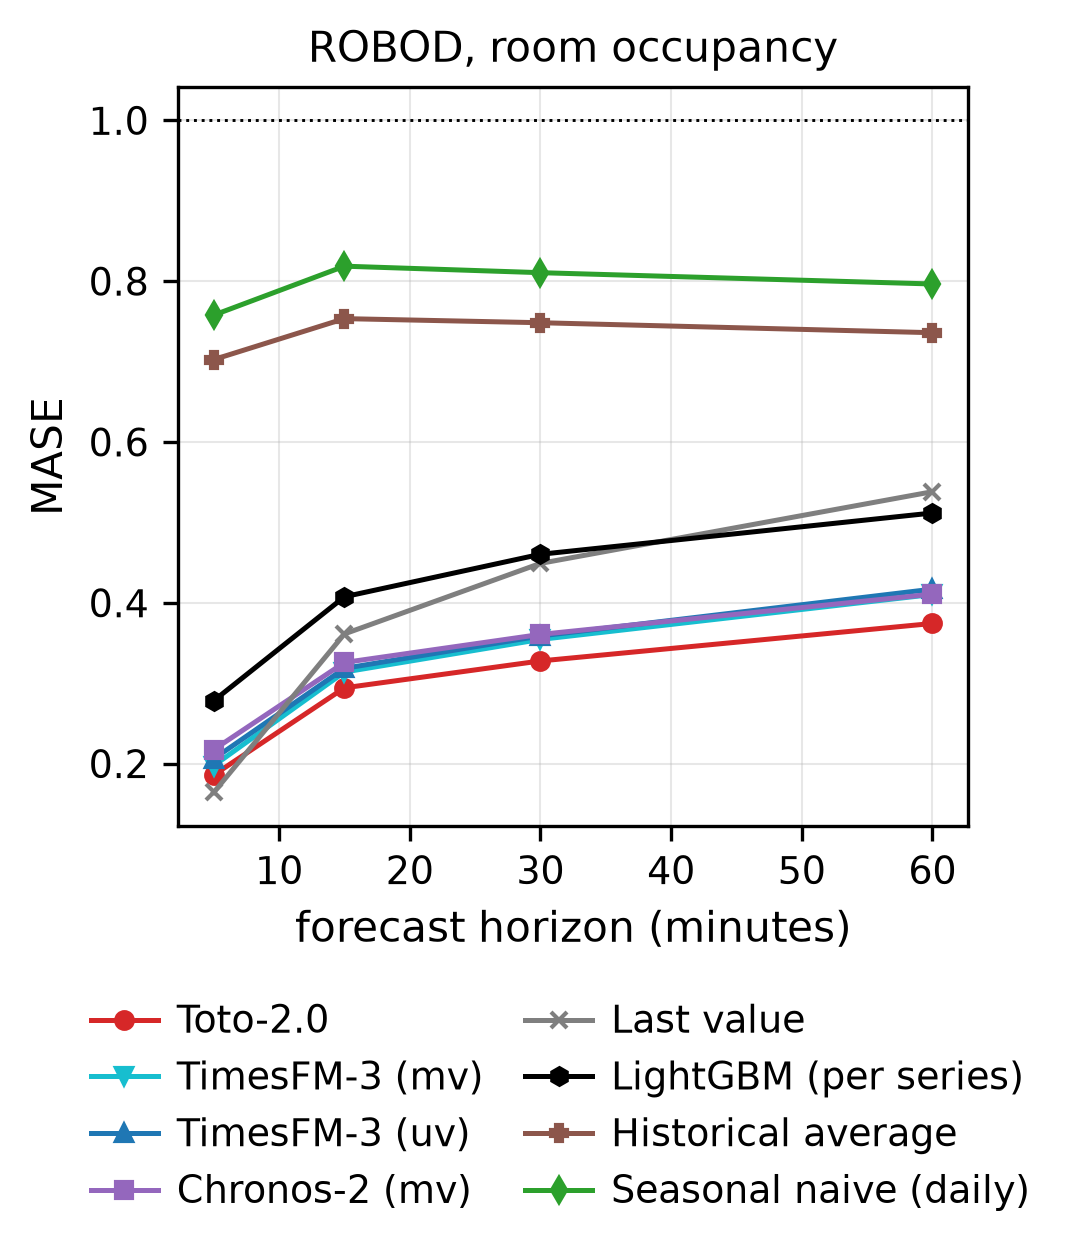
\includegraphics[width=\linewidth]{figures/skill_robod.png}
\caption{ROBOD, $S_m=0.44$.}
\end{subfigure}
\hfill
\begin{subfigure}{0.48\textwidth}
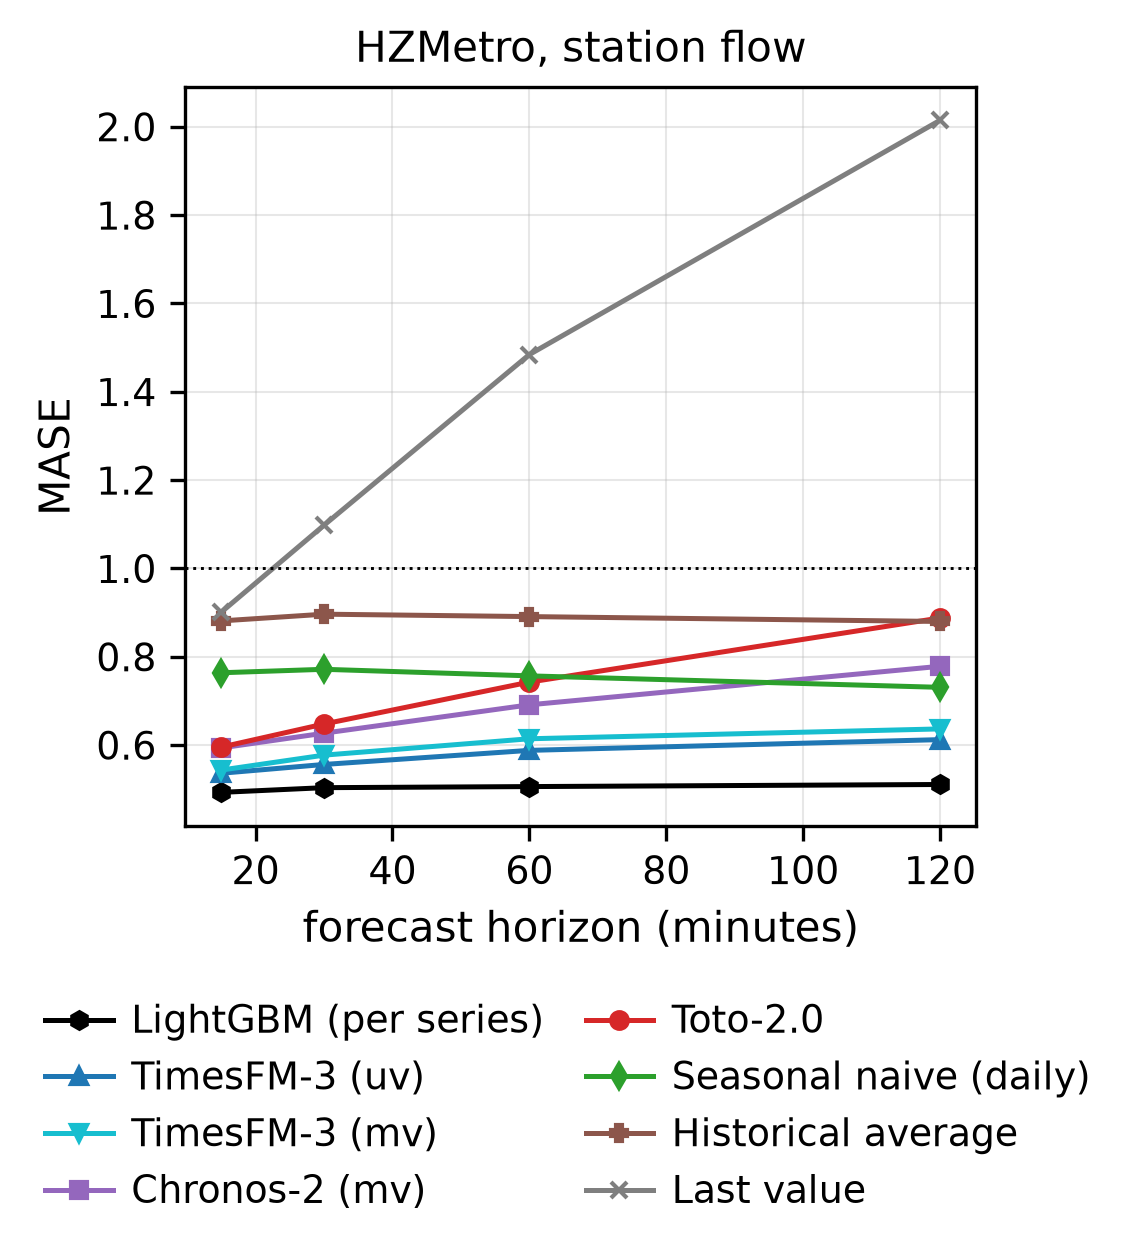
\includegraphics[width=\linewidth]{figures/skill_hzmetro.png}
\caption{HZMetro, $S_m=0.79$.}
\end{subfigure}
\caption{Accuracy against horizon on the two real datasets, with a context of two daily seasons. \new{The foundation models separate from every trivial baseline on both sites, and the separation widens with horizon. The overlaid black line is the per-series gradient-boosted competitor of Section~\ref{sec:lgbm}, which the submitted version of this figure did not include: it stays behind on ROBOD and overtakes the foundation models on HZMetro, which is why the transferability claim is now stated per site rather than as a dominance result.} The dotted line at MASE \num{1} is the in-sample seasonal naive reference. Table~\ref{tab:context} shows how much of the right-hand panel depends on the context length.}
\label{fig:skill}
\end{figure}

Table~\ref{tab:hzmetro} reports HZMetro, where the panel is larger and the tests correspondingly sharper. TimesFM-3 attains \num{0.536} MASE at \SI{15}{\minute} against \num{0.764} for seasonal naive, an improvement of \SI{29.8}{\percent}, and all four foundation model configurations beat the seasonal baseline significantly at \SI{15}{\minute} under Holm control, three of them at \SI{30}{\minute}. Beyond one hour the improvements remain in the range \SIrange{16}{19}{\percent} but are no longer significant at \num{186} and \num{196} origins. \new{The submitted version concluded here that Hypothesis~\ref{hyp:transfer} is supported. It is not. Against the gradient-boosted ladder of Section~\ref{sec:lgbm} the hypothesis fails on this dataset, and we record it as refuted.}

\begin{table}[htbp]
\centering
\caption{HZMetro, real station flow, \num{181}--\num{196} distinct origins depending on horizon. A star marks a significant improvement over the best baseline, seasonal naive, under Diebold-Mariano with Holm control at $\alpha=0.05$ over the seven comparisons at that horizon.}
\label{tab:hzmetro}
\small
\begin{tabular}{lcccccccc}
\toprule
& \multicolumn{4}{c}{MASE} & \multicolumn{4}{c}{CRPS} \\
\cmidrule(lr){2-5}\cmidrule(lr){6-9}
Method & \SI{15}{\minute} & \SI{30}{\minute} & \SI{60}{\minute} & \SI{120}{\minute} & \SI{15}{\minute} & \SI{30}{\minute} & \SI{60}{\minute} & \SI{120}{\minute} \\
\midrule
\multicolumn{9}{l}{\emph{Zero-shot foundation models}}\\
TimesFM-3 (uv)          & \best{0.536}$^{*}$ & \best{0.556}$^{*}$ & \best{0.588} & \best{0.613} & \best{16.51} & \best{17.33} & \best{18.79} & 20.32 \\
TimesFM-3 (mv)          & 0.544$^{*}$ & 0.577$^{*}$ & 0.614 & 0.637 & 16.60 & 17.69 & 18.99 & \best{19.92} \\
Chronos-2 (mv)          & 0.594$^{*}$ & 0.627$^{*}$ & 0.691 & 0.779 & 18.12 & 19.20 & 21.40 & 24.56 \\
Toto-2.0                & 0.596$^{*}$ & 0.648 & 0.743 & 0.888 & 18.07 & 19.94 & 23.22 & 28.62 \\
\midrule
\multicolumn{9}{l}{\emph{Local baselines}}\\
Seasonal naive          & 0.764 & 0.772 & 0.757 & 0.731 & 26.05 & 26.34 & 25.93 & 25.18 \\
LightGBM (trained)      & 0.792 & 0.873 & 1.006 & 1.135 & 25.33 & 28.08 & 32.47 & 36.56 \\
Historical average      & 0.881 & 0.897 & 0.891 & 0.880 & 32.15 & 32.67 & 32.52 & 32.19 \\
Last value              & 0.901 & 1.098 & 1.484 & 2.015 & 30.16 & 37.52 & 52.06 & 72.14 \\
\bottomrule
\end{tabular}
\end{table}

\subsection{\new{How much of H1 was the competitor's specification?}}
\label{sec:lgbm}

\new{A reviewer judged that a single globally trained gradient-boosted model, reported without its training window, lag set, tuning protocol or multi-horizon strategy, was too weak and too undocumented a competitor for Hypothesis~\ref{hyp:transfer} to rest on, and asked for a per-series or direct multi-horizon variant. We agree, and this section is the result. It is the single most consequential change in the revision, because it overturns the paper's headline claim on one of the two real datasets.}

\new{We first disclose the submitted configuration, which Table~\ref{tab:lgbm} calls \emph{as submitted}. One LightGBM model is fitted across all series of a site on the whole training split, with lags $\{1,2,3,5,10,15,30,60,120\}$ steps, rolling means and standard deviations over windows $\{5,15,60\}$, and calendar features for time of day, day of week and a weekend indicator. Hyperparameters are the library defaults with \num{31} leaves, learning rate \num{0.05} and \num{300} trees. Multi-horizon forecasts come from one model per step trained on a fixed subset of steps, with intermediate steps interpolated. Quantiles come from nine separate pinball objectives. Nothing in that specification is tailored to a daily or weekly period, and nothing is tuned.}

\new{We then build a ladder of four increasingly careful specifications, each adding exactly one change so that the contributions are separable.}
\new{\begin{description}
\item[Horizon matched.] A separate model for every forecast step up to the maximum horizon, removing the interpolation across steps.
\item[Seasonal lags.] Adds lags at the daily period and its neighbours, $\{m-1, m, m+1, 2m\}$, and at the weekly period $\{7m-1, 7m, 7m+1\}$, where $m$ is the number of steps in a day. On HZMetro at fifteen minutes this adds lags \num{95}, \num{96}, \num{97}, \num{192}, \num{671}, \num{672} and \num{673}. The submitted feature set reached back \num{120} steps, which on HZMetro is \SI{30}{\hour} and therefore could not see the previous day at the same time of day at all.
\item[Tuned.] A grid of six configurations over the number of leaves, the learning rate, the number of trees and the minimum leaf occupancy, selected by median pinball loss on the final fifth of the training design matrix, which is held out from fitting. Selection never touches the test split.
\item[Per series.] One model per series rather than one model across series, with the tuned configuration and the seasonal lag set.
\end{description}}

\new{\begin{table}[htbp]
\centering
\caption{\new{The gradient-boosted ladder, MASE, lower better. Each row adds one change to the row above it within the LightGBM block. The strongest zero-shot configuration for each dataset and the strongest untrained baseline are shown for reference. Identical origins, context, stride and horizon grid as Tables~\ref{tab:robod} and~\ref{tab:hzmetro}.}}
\label{tab:lgbm}
\small
\begin{tabular}{lcccc}
\toprule
\multicolumn{5}{l}{\emph{(a) HZMetro, station flow, \num{196} origins}}\\
Method & \SI{15}{\minute} & \SI{30}{\minute} & \SI{60}{\minute} & \SI{120}{\minute} \\
\midrule
LightGBM, as submitted      & 0.792 & 0.873 & 1.006 & 1.135 \\
\quad + horizon matched     & 0.719 & 0.771 & 0.867 & 0.996 \\
\quad + seasonal lags       & 0.635 & 0.640 & 0.735 & 0.899 \\
\quad + tuned               & 0.581 & 0.587 & 0.673 & 0.805 \\
\quad + per series          & \best{0.493} & \best{0.504} & \best{0.506} & \best{0.511} \\
\midrule
TimesFM-3 (uv), zero-shot   & 0.536 & 0.556 & 0.588 & 0.613 \\
Seasonal naive              & 0.764 & 0.772 & 0.757 & 0.731 \\
\midrule
\multicolumn{5}{l}{\emph{(b) ROBOD, room occupancy, \num{261} origins}}\\
Method & \SI{5}{\minute} & \SI{15}{\minute} & \SI{30}{\minute} & \SI{60}{\minute} \\
\midrule
LightGBM, as submitted      & 0.263 & 0.439 & 0.517 & 0.601 \\
\quad + horizon matched     & 0.231 & 0.406 & 0.480 & 0.550 \\
\quad + seasonal lags       & 0.237 & 0.411 & 0.487 & 0.556 \\
\quad + tuned               & 0.226 & 0.403 & 0.481 & 0.551 \\
\quad + per series          & 0.278 & 0.407 & 0.460 & 0.512 \\
\midrule
Toto-2.0, zero-shot         & 0.186 & \best{0.294} & \best{0.328} & \best{0.374} \\
Last value                  & \best{0.164} & 0.361 & 0.449 & 0.538 \\
\bottomrule
\end{tabular}
\end{table}}

\new{\paragraph{On HZMetro the hypothesis fails.} The ladder at two hours runs \num{1.135}, \num{0.996}, \num{0.899}, \num{0.805}, \num{0.511}, so re-specification cuts the error by more than half. The per-series arm reaches \num{0.511} against \num{0.613} for the best zero-shot configuration, \rev{a reduction of \SI{16.6}{\percent} in favour of the local model by definition~\eqref{eq:relimp}, with the zero-shot MASE as the reference}, and it leads at every one of the four horizons\rev{, by \SI{8.1}{\percent}, \SI{9.4}{\percent}, \SI{13.9}{\percent} and \SI{16.6}{\percent} from the shortest to the longest}. The advantage carries $p=\num{1.4e-2}$ and survives Holm control across the comparisons at that horizon. \rev{An earlier version of this revision gave this advantage as \SI{28.9}{\percent}, and a reviewer correctly observed that the MASE values beside it imply about \SI{16.6}{\percent}. The discrepancy came from mixing two quantities. The significance test is computed on the paired per-origin MAE, which is \num{23.61} passengers per interval for the local model and \num{30.43} for the zero-shot model over the \num{196} origins, and \SI{28.9}{\percent} was the excess of the larger of these over the smaller, $100(30.43/23.61 - 1)$: a different loss and a different denominator from those of every other percentage in the paper. On the paired MAE the reduction under definition~\eqref{eq:relimp} is \SI{22.4}{\percent}, and on the per-series MASE of Table~\ref{tab:lgbm} it is \SI{16.6}{\percent}. The two differ because MASE divides each series by its own scale before averaging, whereas the mean MAE is dominated by the busiest stations. We report the MASE figure throughout, since it is the quantity tabulated, and the test statistic and its $p$-value are unaffected.} We checked for leakage rather than assuming its absence, since a local model that suddenly beats a foundation model is exactly the situation in which one should look: the training split ends at step \num{1896}, the test split starts at \num{1904} with a gap of eight steps equal to the longest horizon, and the first scored origin is \num{1914}, so no training row can contain a test observation. The result stands. The largest single step in the ladder is the per-series one, which is consistent with the obvious reading: \num{160} metro flow series with strong but station-specific daily profiles are better served by \num{160} small models than by one model asked to represent all of them, and the submitted global arm was the wrong shape for this dataset rather than merely untuned.}

\new{\paragraph{On ROBOD the hypothesis survives.} The same ladder moves the error from \num{0.601} to \num{0.512} at one hour, an improvement of \SI{14.8}{\percent}, which is real but leaves Toto-2.0 at \num{0.374} ahead by \rev{\SI{26.9}{\percent} on MASE (\SI{26.8}{\percent} on the paired per-origin MAE, \num{0.450} against \num{0.615} persons)}. Two things are worth recording. The per-series arm now beats last value, \num{0.512} against \num{0.538}, so the submitted sentence that the trained model ``does not even reach last value'' is withdrawn; it was an artefact of the specification. And the margin over the best local arm, while large, no longer survives Holm control at $\alpha = 0.05$ on \num{261} origins, which is consistent with what Section~\ref{sec:h1} already said about the inferential power of this dataset.}

\new{\paragraph{What we conclude instead.} The honest summary is that the zero-shot advantage is real but conditional, and that the condition is not the one the submitted paper proposed. It is not primarily about how much local data exists, as Section~\ref{sec:efficiency} shows directly. It is about whether the local model has been given the right shape for the target: a specification that matches the series' own periodicity and granularity closes most of the gap, and on a large, strongly periodic, station-level panel it closes all of it and more. The claim that survives is the one in Section~\ref{sec:disc}, and it is narrower.}

\subsection{The comparison is decided by context length}
\label{sec:context}

The HZMetro column above reverses a conclusion we had previously drawn from the identical protocol, and the only difference is the length of the context window. Table~\ref{tab:context} places the two runs side by side.

\begin{table}[htbp]
\centering
\caption{The same models, the same origins, the same metric, at one and at two daily seasons of context on HZMetro. MASE, lower is better. The methods that read only the last observation are unaffected by construction, and the seasonal baseline barely moves, so the change is not a change in the difficulty of the task.}
\label{tab:context}
\small
\begin{tabular}{lcccc@{\hskip 2em}cccc}
\toprule
& \multicolumn{4}{c}{context $=m$ (one season)} & \multicolumn{4}{c}{context $=2m$ (two seasons)} \\
\cmidrule(lr){2-5}\cmidrule(lr){6-9}
Method & \SI{15}{\minute} & \SI{30}{\minute} & \SI{60}{\minute} & \SI{120}{\minute} & \SI{15}{\minute} & \SI{30}{\minute} & \SI{60}{\minute} & \SI{120}{\minute} \\
\midrule
TimesFM-3 (uv)     & 0.720 & 0.793 & 0.898 & 0.963 & \best{0.536} & \best{0.556} & \best{0.588} & \best{0.613} \\
TimesFM-3 (mv)     & 0.690 & 0.785 & 0.903 & 0.972 & 0.544 & 0.577 & 0.614 & 0.637 \\
Chronos-2 (mv)     & 0.943 & 1.110 & 1.486 & 2.064 & 0.594 & 0.627 & 0.691 & 0.779 \\
Toto-2.0           & 0.758 & 0.902 & 1.211 & 1.719 & 0.596 & 0.648 & 0.743 & 0.888 \\
\midrule
Seasonal naive     & 0.759 & 0.766 & 0.750 & 0.722 & 0.764 & 0.772 & 0.757 & 0.731 \\
Last value         & 0.901 & 1.098 & 1.484 & 2.015 & 0.901 & 1.098 & 1.484 & 2.015 \\
\bottomrule
\end{tabular}
\end{table}

At one season the seasonal baseline beats every foundation model at every horizon beyond \SI{15}{\minute}, and at \SI{120}{\minute} it beats the best of them by \SI{25}{\percent}. At two seasons the same models beat it by \SI{16}{\percent}. Chronos-2 improves by a factor of \num{2.6} at the longest horizon. Nothing about the task changed: the origins, the truth, the metric and the seasonal denominator are identical, and last value is numerically unchanged because it reads a single point.

\new{\paragraph{Does the improvement continue, saturate or reverse?} Two reviewers observed that two context lengths on one dataset cannot answer this, and that the submitted conclusion therefore rested on the narrowest possible evidence. One also noted that the local baselines were given at most two days of context while the metro has pronounced weekly seasonality, so the seasonal baseline was the daily one throughout and a weekly baseline was never run. Both are fair and Table~\ref{tab:sweep} answers them. We ran the full protocol at one, two, three, seven and fourteen daily seasons of context on both real datasets, and added a weekly seasonal baseline wherever the context is long enough to define one, which requires at least fourteen daily seasons.}

\new{\begin{table}[htbp]
\centering
\caption{\new{The context sweep. MASE at the longest horizon of each dataset, \SI{120}{\minute} on HZMetro and \SI{60}{\minute} on ROBOD, against context length in daily seasons. Origins are held common across all five contexts: all \num{196} on HZMetro and the \num{261} shared by every context on ROBOD, so each row is a paired comparison. The weekly seasonal baseline is defined only at fourteen daily seasons, which is the shortest context containing two weekly periods.}}
\label{tab:sweep}
\small
\begin{tabular}{lccccc}
\toprule
& \multicolumn{5}{c}{context length, in daily seasons}\\
\cmidrule(lr){2-6}
Method & 1 & 2 & 3 & 7 & 14 \\
\midrule
\multicolumn{6}{l}{\emph{(a) HZMetro, station flow, \SI{120}{\minute}, \num{196} common origins}}\\
TimesFM-3 (uv)         & 1.037 & 0.677 & 0.557 & 0.424 & \best{0.414} \\
TimesFM-3 (mv)         & 1.042 & 0.665 & 0.584 & 0.448 & 0.433 \\
Chronos-2 (mv)         & 2.214 & 0.827 & 0.673 & 0.470 & 0.426 \\
Toto-2.0               & 1.842 & 0.919 & 0.788 & 0.656 & 0.593 \\
\midrule
Seasonal naive (daily) & 0.774 & 0.781 & 0.777 & 0.774 & 0.774 \\
\new{Seasonal naive (weekly)} & n/a & n/a & n/a & n/a & 0.598 \\
Historical average     & 0.924 & 0.900 & 0.601 & 0.487 & 0.541 \\
Last value             & 2.155 & 2.155 & 2.155 & 2.155 & 2.155 \\
\midrule
\multicolumn{6}{l}{\emph{(b) ROBOD, room occupancy, \SI{60}{\minute}, \num{261} common origins}}\\
Toto-2.0               & 0.454 & 0.374 & 0.358 & 0.310 & \best{0.309} \\
TimesFM-3 (mv)         & 0.508 & 0.409 & 0.389 & 0.315 & 0.314 \\
TimesFM-3 (uv)         & 0.476 & 0.413 & 0.406 & 0.336 & 0.332 \\
Chronos-2 (mv)         & 0.470 & 0.412 & 0.392 & 0.348 & 0.346 \\
\midrule
Seasonal naive (daily) & 0.761 & 0.814 & 0.761 & 0.761 & 0.761 \\
\new{Seasonal naive (weekly)} & n/a & n/a & n/a & n/a & 0.887 \\
Historical average     & 0.818 & 0.749 & 0.618 & 0.650 & 0.745 \\
Last value             & 0.529 & 0.529 & 0.529 & 0.529 & 0.529 \\
\bottomrule
\end{tabular}
\end{table}}

\new{The answer is that the improvement continues well past two seasons and then saturates, and that it never reverses. On HZMetro the best configuration runs \num{1.037}, \num{0.677}, \num{0.557}, \num{0.424}, \num{0.414} as the context grows, reaching within \SI{2.5}{\percent} of its final value by seven daily seasons; on ROBOD the pattern is the same shape, \num{0.454}, \num{0.374}, \num{0.358}, \num{0.310}, \num{0.309}. The submitted paper's two-point comparison therefore caught the steepest part of a curve and stopped, and the choice of two seasons, which we had defended as adequate, in fact left about two fifths of the available improvement unused. The qualitative conclusion is unchanged and the quantitative one is stronger than we claimed. Throughout, the baselines that read only the last observation are flat to four decimal places and the daily seasonal baseline moves by less than \SI{1}{\percent}, so the task itself is unchanged across the sweep, which is the control that makes the comparison interpretable. The one non-monotone row is historical average, which improves to three seasons and then degrades, as a time-of-day mean over a longer window begins to average across genuinely different days.}

\new{\paragraph{The weekly baseline is a much stronger competitor, and still loses.} On HZMetro a weekly seasonal naive forecast reaches \num{0.598} MASE against \num{0.774} for the daily one, an improvement of \SI{22.7}{\percent}, which confirms the reviewer's point that restricting the baselines to a daily lag understated them. It remains \SI{30.8}{\percent} behind the best zero-shot configuration at the same context. On ROBOD the weekly baseline is \emph{worse} than the daily one, \num{0.887} against \num{0.761}, which is what one should expect given that ROBOD's usable record is a sequence of weekday blocks interrupted by a two-month gap, so the observation one week earlier is frequently missing or drawn from a different occupancy regime. We report both because the contrast is informative: the weekly baseline is the right competitor on a metro network and the wrong one on this building, and a paper that ran only the daily version would have been flattering itself on HZMetro.}

We draw two conclusions, and regard them as among the paper's more useful outputs.

First, a zero-shot evaluation on periodic data is not interpretable without its context length, and a context of one seasonal period is a specific and unfavourable choice rather than a neutral one. A model that has seen one instance of the daily profile cannot distinguish the profile from the noise around it, and the models here evidently use the second instance to do exactly that. Reported comparisons between foundation models and seasonal baselines should state the context in units of the season and, where the claim matters, vary it. \new{Table~\ref{tab:sweep} strengthens this: the sensitivity does not stop at the point where the comparison flips, so a study that happens to pick two seasons is not safe either, and the honest practice is to report the curve.}

\new{A third point, which a reviewer raised and which we cannot resolve from inside this study, concerns pretraining contamination. HZMetro is a public benchmark released in 2022 and the foundation models evaluated here were pretrained on undisclosed corpora assembled later. We therefore cannot exclude that some of these series, or close relatives of them, appear in some model's training data, which would make the HZMetro comparison not strictly zero-shot. Three observations bound the concern without removing it. The context sensitivity in Table~\ref{tab:sweep} is hard to reconcile with memorisation, since a model that had memorised these series would not need seven daily periods of context to forecast them. The ROBOD result, on a dataset of room occupancy counts in a format far from any public forecasting corpus, is qualitatively identical. And the models disagree with each other substantially on HZMetro, by up to \SI{43}{\percent} at the longest horizon, which is not the pattern one expects if they were all reciting the same memorised series. We nonetheless regard the ROBOD result as the cleaner evidence for Hypothesis~\ref{hyp:transfer}, and we note that until pretraining corpora are disclosed, no evaluation of a foundation model on a public benchmark can fully exclude this, which is a limitation of the field rather than of this paper.}

Second, the same choice silently disarms the baselines. At a context of exactly $m$, the residual series $y_t - y_{t-m}$ that a seasonal naive method needs to form a prediction interval is empty, and a time-of-day mean has one observation per bucket and therefore residuals that are identically zero. In our first run both baselines were consequently scored with zero-width intervals and covered a few percent of outcomes, which we would have reported as evidence that they are uncalibrated. They are not: at two seasons, seasonal naive covers \SI{83.9}{\percent} of outcomes on ROBOD against a nominal \SI{80}{\percent}. An evaluation that starves a baseline of its uncertainty and then reports it as overconfident has measured its own configuration.

\subsection{H2: the predictability boundary, \rev{not supported}}

We \new{stated a priori} the claim that the zero-shot advantage declines with the daily seasonal strength of the target. Across datasets the pattern is not even ordered: the advantage is $+\SI{30.5}{\percent}$ at $S_m=0.44$ on ROBOD, $-\new{\SI{5.3}{\percent}}$ at $S_m=0.55$ on the simulator and $+\SI{16.2}{\percent}$ at $S_m=0.79$ on HZMetro, so the highest-$S_m$ dataset is not the one where the models do worst. That alone is not decisive, since three points with different sensors, scales and reference baselines cannot separate $S_m$ from everything else that distinguishes them, and Remark~\ref{rem:sim} forbids using the simulator for a transfer claim in any case.

The test that can separate them is within a dataset. Figure~\ref{fig:within} regresses the per-series MAE advantage of a fixed foundation model over a fixed seasonal baseline on per-series $S_m$, holding dataset identity constant. On HZMetro's \num{160} flow series the slope is $-17$ percentage points per unit $S_m$ with a \SI{95}{\percent} confidence interval of $[-38, +4]$, $p=\num{0.12}$ and $R^2=\num{0.015}$; the rank correlation is $\rho=-0.17$. On ROBOD's five series nothing can be concluded. The sign is in the predicted direction and the magnitude is not negligible, but the relationship explains one and a half percent of the variance in the advantage and is not distinguishable from zero. \rev{\textbf{Hypothesis~\ref{hyp:boundary} is not supported by the within-dataset analysis, and we do not rely on it.} We choose these words deliberately. The falsification criterion we stated, a slope not distinguishable from zero, is met, so the hypothesis fails the test we set for it. That is a failure to establish the relationship and not a demonstration that it is absent. The interval $[-38, +4]$ is wide: across the observed range of $S_m$ on this panel, \num{0.57} to \num{0.89}, its lower end corresponds to a decline of about twelve percentage points in the advantage, which would be operationally relevant against a median advantage of \SI{14.3}{\percent}, and its upper end to a rise of about one point. The rank correlation points the same way: $\rho=-0.17$ carries $p=\num{0.032}$ taken alone, which we do not read as confirmation, since the slope and not the rank correlation was the test specified in advance and the pair is not corrected for multiplicity, but which is a further reason not to describe the hypothesis as disproved. The data are therefore compatible both with no dependence and with a meaningful negative dependence, the predictor varies over a range of only \num{0.32} on this panel, and a single panel of one kind of series cannot decide between them. The accurate statement is that the dependence is not statistically established.}

\begin{figure}[htbp]
\centering
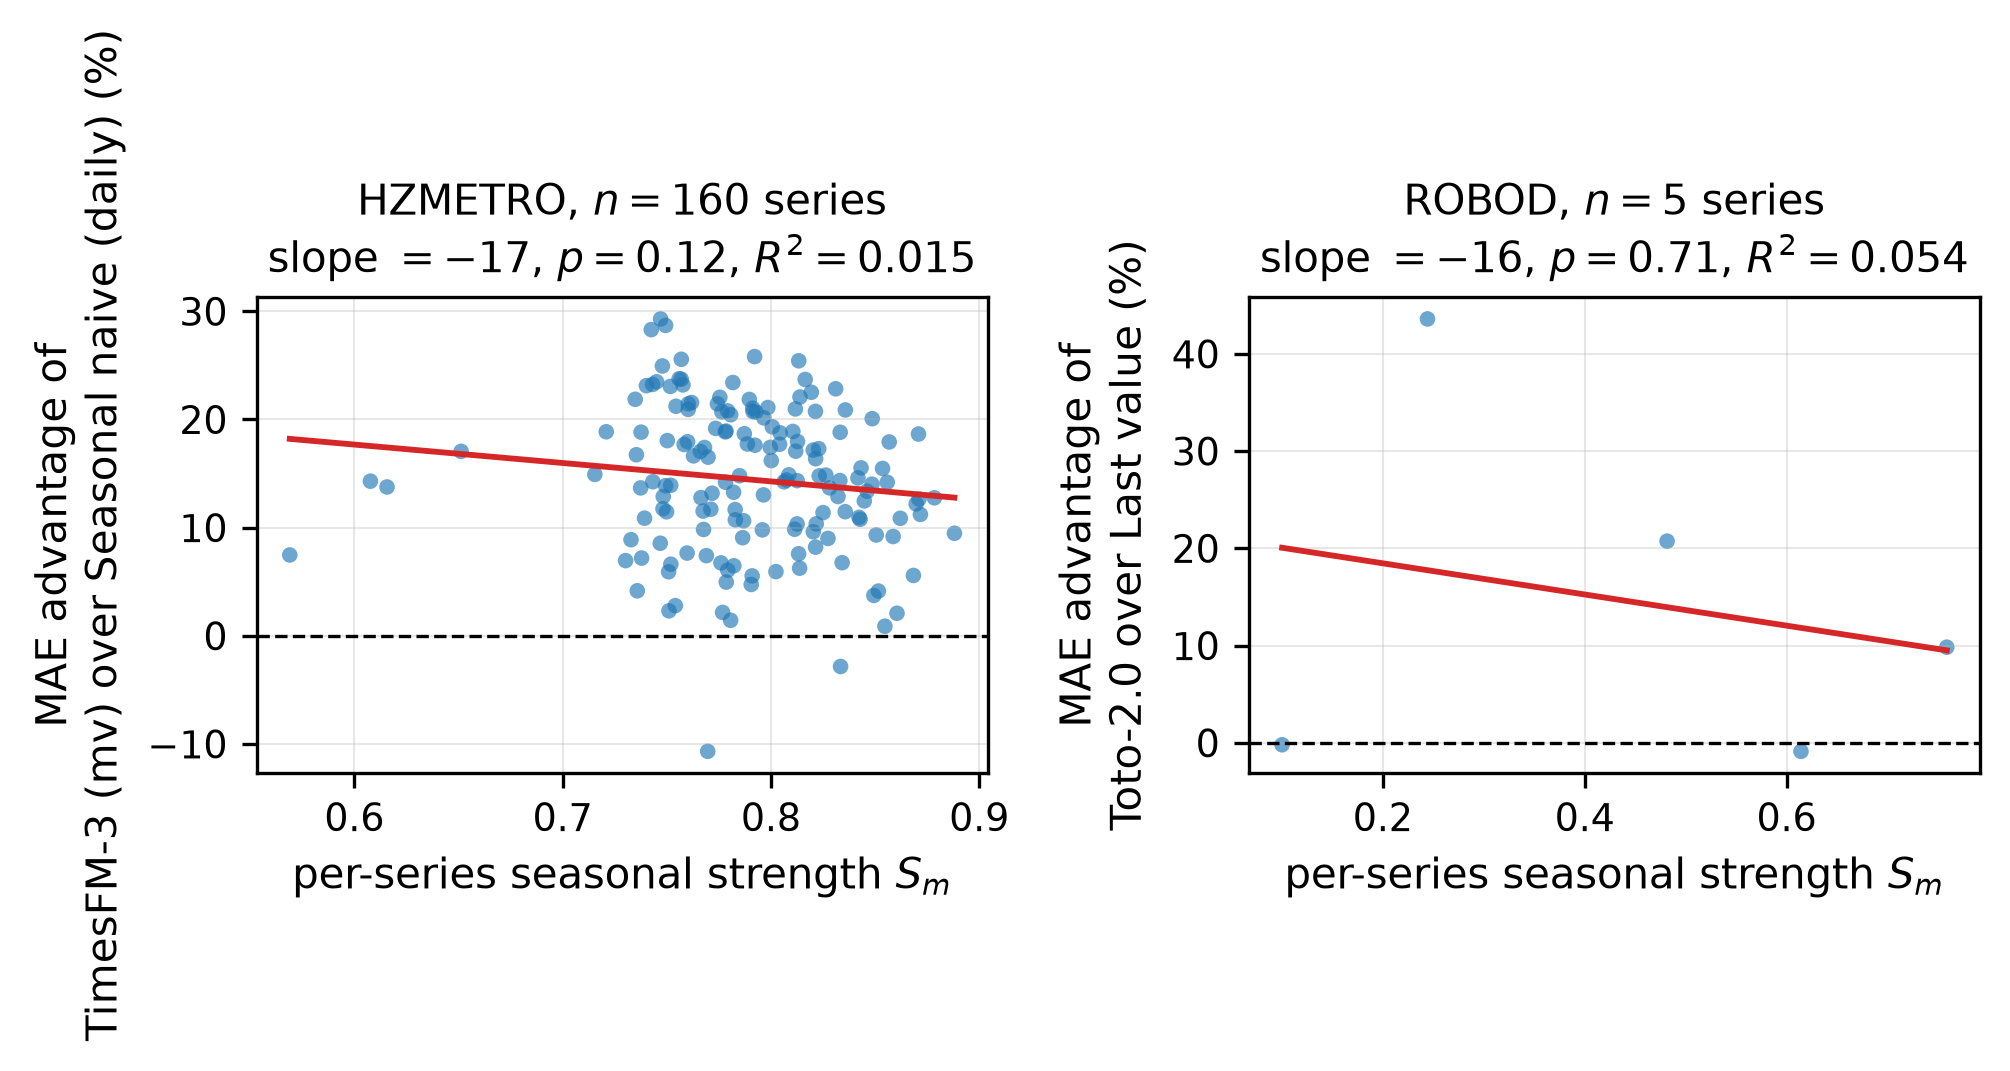
\includegraphics[width=0.92\textwidth]{figures/within_dataset.png}
\caption{The within-dataset test of Hypothesis~\ref{hyp:boundary}. Each point is one series; the vertical axis is the percentage reduction in MAE of a fixed zero-shot model over a fixed seasonal baseline, and the horizontal axis is that series' daily seasonal strength. The regression line is negative on both panels and distinguishable from zero on neither. The figure also shows, incidentally, the strongest evidence for Hypothesis~\ref{hyp:transfer} in the paper: \num{158} of \num{160} HZMetro series lie above zero.}
\label{fig:within}
\end{figure}

Two remarks on why we think this is the right outcome rather than a disappointing one. The between-dataset version of the claim was close to circular: $S_m$ is defined as the variance fraction explained by the daily profile and the competing baseline \emph{is} the daily profile, so asserting that the advantage over that baseline falls as $S_m$ rises largely restates the definition. The within-dataset test is the version that could have failed, and it \rev{did not support the claim}. And the figure delivers something the ordering never could: across \num{160} series spanning $S_m$ from \num{0.57} to \num{0.89}, the zero-shot advantage is positive on \num{158} of them, with a median of \SI{14.3}{\percent}, and has no \rev{statistically established} dependence on periodicity. The useful claim is therefore the unconditional one we tried to avoid making, which the data now supports far better than the conditional one we preferred.

\subsection{H3: sharper intervals at matched coverage}

Point accuracy is not what a protection system consumes. An alarm rule needs the probability that a threshold will be crossed, and that requires a calibrated distribution. Table~\ref{tab:calibration} reports coverage and width against baselines that form their intervals from their own residual quantiles, which is the comparison Hypothesis~\ref{hyp:uncertainty} is stated against.

\begin{table}[htbp]
\centering
\caption{Empirical coverage of the nominal \SI{80}{\percent} interval, with mean interval width in persons on ROBOD and in passengers per interval on HZMetro. Every method here forms intervals from its own uncertainty, the baselines from the empirical quantiles of their in-context residuals. Coverage alone cannot be read as quality: an arbitrarily wide interval covers everything, so the pair matters.}
\label{tab:calibration}
\small
\begin{tabular}{lcccc}
\toprule
& \multicolumn{2}{c}{ROBOD (\SI{60}{\minute})} & \multicolumn{2}{c}{HZMetro (\SI{60}{\minute})} \\
\cmidrule(lr){2-3}\cmidrule(lr){4-5}
Method & coverage & width & coverage & width \\
\midrule
Toto-2.0            & 0.901 & \best{1.17} & 0.824 & 121.2 \\
TimesFM-3 (mv)      & 0.892 & 1.19 & 0.756 & \best{87.7} \\
TimesFM-3 (uv)      & 0.890 & 1.27 & 0.771 & 94.3 \\
Chronos-2 (mv)      & 0.912 & 1.45 & 0.829 & 112.2 \\
\midrule
Seasonal naive      & 0.839 & 2.35 & 0.706 & 83.7 \\
LightGBM (trained)  & 0.944 & 1.90 & 0.820 & 183.1 \\
Historical average  & 0.696 & 0.61 & 0.379 & 24.8 \\
Last value          & 0.821 & 0.06 & 0.597 & 85.1 \\
\bottomrule
\end{tabular}
\end{table}

\new{\paragraph{The calibration claim does not hold, and the sharpness claim does.}
\label{sec:calib}
The submitted version read Table~\ref{tab:calibration} as showing that on ROBOD the foundation model is ``better calibrated \emph{and} twice as sharp''. A reviewer pointed out that the first half is refuted by the very numbers quoted: seasonal naive covers \SI{83.9}{\percent} and Toto-2.0 covers \SI{90.1}{\percent} against a nominal \SI{80}{\percent}, so the deviation from nominal is \num{3.9} points for the baseline and \num{10.1} points for the foundation model, and the baseline is the better calibrated of the two. The claim was wrong and we withdraw it. Toto-2.0 overcovers, which is to say its intervals are too wide for their nominal level, and the honest description is that it is \emph{miscalibrated in the safe direction}.}

\new{Correcting this requires separating two things the submitted table conflated. Calibration is the distance from nominal coverage. Sharpness is width. A method can win on either while losing on the other, and comparing raw widths across methods with different coverages compares nothing, because a wider interval covering more outcomes is not thereby worse. Table~\ref{tab:matched} therefore rescales each method's interval about its own median \rev{and reports the width at a common target coverage. An earlier version of this table was computed inconsistently and a reviewer identified the symptom. The table, the procedure behind it and the conclusions drawn from it are replaced here.}}

\rev{\paragraph{What was wrong with the earlier table.} The earlier table listed seasonal naive on ROBOD with an empirical coverage of \num{0.839} and a scale factor of \num{1.60} to reach \num{0.80}. As the reviewer observed, that is impossible: scaling an interval about its median by a factor above one can only add outcomes to it, so a method already covering more than the target needs a factor of at most one. The cause was that the two columns were computed on different observations by different rules. Coverage was computed on all observations. The factor was the \num{80}th percentile of the absolute error divided by half the interval width, computed only on the observations whose interval had positive width, which for seasonal naive on ROBOD is \SI{57}{\percent} of them, and with half the total width in place of the half-width on the side of the error. A factor obtained in that way does not bring the coverage of the full sample to \num{0.80}: applied to all observations it gave \num{0.844} for seasonal naive and \num{0.836} for Toto-2.0. The width of \num{3.75} persons, and the ratio of \num{4.9} derived from it, were therefore not widths at a matched coverage, and both are withdrawn. The factors were also estimated on the evaluation observations themselves, which the earlier text did not state.}

\rev{\paragraph{The rescaling rule.} For an observation with quantile forecasts $q^{0.1} \le q^{0.5} \le q^{0.9}$ and outcome $y$, the interval scaled by a factor $f \ge 0$ is $[\,q^{0.5} - f(q^{0.5}-q^{0.1}),\; q^{0.5} + f(q^{0.9}-q^{0.5})\,]$, each side being scaled separately so that an asymmetric interval keeps its shape. The smallest factor at which the outcome is covered is the score
\begin{equation}
s \;=\; \begin{cases} (q^{0.5}-y)/(q^{0.5}-q^{0.1}), & y < q^{0.5},\\[2pt] 0, & y = q^{0.5},\\[2pt] (y-q^{0.5})/(q^{0.9}-q^{0.5}), & y > q^{0.5},\end{cases}
\label{eq:score}
\end{equation}
with $s=\infty$ when the outcome lies on a side of zero width, in which case no rescaling covers it. The outcome is covered at factor $f$ exactly when $s \le f$, so the empirical coverage as a function of $f$ is the empirical distribution function of the scores over \emph{all} observations. It is non-decreasing in $f$ by construction, and at $f=1$ it equals the published coverage identically, which the analysis script asserts for every method before reporting anything. Two estimates of the factor are reported. The \emph{retrospective} factor is the smallest $f$ whose coverage on the evaluation observations is at least the target $c$, that is the $\lceil cn\rceil$-th smallest of the $n$ scores. It is estimated on the same observations on which the width is then reported, so it describes the forecasts after the fact and could not have been applied in operation. The \emph{out-of-sample} factor is the split conformal quantile \citep{vovk2005}, the $\lceil c(n_{\mathrm{cal}}+1)\rceil$-th smallest score on a calibration period, applied unchanged to a later evaluation period. We report it in two forms. In the single split the first half of the test origins calibrates and the second half evaluates, with $\lceil h/s\rceil$ origins removed between them, for horizon $h$ and stride $s$ in steps, so that no calibration target window overlaps an evaluation one. In the expanding window the factor applied at an origin is estimated from all earlier origins outside that gap, after a burn-in of one quarter of the origins. The foundation models remain zero-shot in both: a single scalar per method is estimated, never from the observations on which it is evaluated.}

\rev{\begin{table}[htbp]
\centering
\revcolor
\caption{\rev{Calibration and sharpness separated, corrected. Horizon \SI{60}{\minute}, observations pooled over series, steps and origins: \num{15660} observations from \num{261} origins on ROBOD and \num{114880} from \num{186} origins on HZMetro. \emph{Published} is the interval as issued, at nominal \SI{80}{\percent}. $f$ is the factor applied to the interval about its median by rule~\eqref{eq:score}; a factor above one widens and can only raise coverage. \emph{Retrospective}: $f$ is the smallest factor reaching the target on the evaluation observations themselves. \emph{Split}: $f$ is estimated on the first half of the origins (\num{130} on ROBOD, \num{93} on HZMetro) and applied to the second half (\num{130} and \num{91}); coverage and width are those of the second half only and are not comparable with the retrospective columns. \emph{Expanding}: each origin is scaled by a factor estimated on earlier origins (\num{195} and \num{138} origins scored). Widths are in persons on ROBOD and passengers per interval on HZMetro. An entry of n/a means that no finite factor reaches the target. Pooled coverage on HZMetro differs in the third decimal from Table~\ref{tab:calibration}, which averages per-origin values.}}
\label{tab:matched}
\scriptsize
\setlength{\tabcolsep}{3.2pt}
\begin{tabular}{lcc@{\hspace{9pt}}ccc@{\hspace{9pt}}ccc@{\hspace{9pt}}cc}
\toprule
& \multicolumn{2}{c}{Published} & \multicolumn{3}{c}{Retrospective} & \multicolumn{3}{c}{Out of sample, split} & \multicolumn{2}{c}{Expanding} \\
\cmidrule(lr){2-3}\cmidrule(lr){4-6}\cmidrule(lr){7-9}\cmidrule(lr){10-11}
Method & cov. & width & $f$ & cov. & width & $f$ & cov. & width & cov. & width \\
\midrule
\multicolumn{11}{l}{\emph{(a) ROBOD, room occupancy, target coverage \num{0.80}}}\\
Toto-2.0            & 0.901 & 1.17 & 1.00 & 0.901 & 1.17 & 1.00 & 0.911 & 1.38 & 0.907 & 1.28 \\
TimesFM-3 (mv)      & 0.892 & 1.19 & 1.00 & 0.892 & 1.19 & 1.00 & 0.895 & 1.40 & 0.894 & 1.29 \\
TimesFM-3 (uv)      & 0.890 & 1.27 & 1.00 & 0.890 & 1.27 & 1.00 & 0.894 & 1.47 & 0.893 & 1.37 \\
Chronos-2 (mv)      & 0.912 & 1.45 & 1.00 & 0.912 & 1.45 & 1.00 & 0.918 & 1.67 & 0.916 & 1.52 \\
LightGBM (trained)  & 0.944 & 1.90 & 1.00 & 0.944 & 1.90 & 0.81 & 0.735 & 1.74 & 0.800 & 1.76 \\
Seasonal naive      & 0.839 & 2.35 & 1.00 & 0.839 & 2.35 & 1.00 & 0.846 & 2.46 & 0.853 & 2.52 \\
Historical average  & 0.696 & 0.61 & 21.50 & 0.800 & 13.10 & n/a & n/a & n/a & n/a & n/a \\
Last value          & 0.821 & 0.06 & 0.00 & 0.815 & 0.00 & 0.00 & 0.812 & 0.00 & 0.814 & 0.00 \\
\midrule
\multicolumn{11}{l}{\emph{(b) ROBOD, room occupancy, target coverage \num{0.90}}}\\
Toto-2.0            & 0.901 & 1.17 & 1.00 & 0.901 & 1.17 & 1.06 & 0.921 & 1.47 & 0.915 & 1.34 \\
TimesFM-3 (mv)      & 0.892 & 1.19 & 1.06 & 0.900 & 1.25 & 1.08 & 0.909 & 1.51 & 0.907 & 1.40 \\
TimesFM-3 (uv)      & 0.890 & 1.27 & 1.08 & 0.900 & 1.37 & 1.11 & 0.909 & 1.63 & 0.910 & 1.55 \\
Chronos-2 (mv)      & 0.912 & 1.45 & 1.00 & 0.912 & 1.45 & 1.00 & 0.918 & 1.67 & 0.916 & 1.52 \\
LightGBM (trained)  & 0.944 & 1.90 & 1.00 & 0.944 & 1.90 & 1.00 & 0.942 & 2.14 & 0.943 & 2.01 \\
Seasonal naive      & 0.839 & 2.35 & 3.00 & 0.902 & 7.04 & 5.00 & 0.919 & 12.28 & n/a & n/a \\
Historical average  & 0.696 & 0.61 & n/a & n/a & n/a & n/a & n/a & n/a & n/a & n/a \\
Last value          & 0.821 & 0.06 & n/a & n/a & n/a & n/a & n/a & n/a & n/a & n/a \\
\midrule
\multicolumn{11}{l}{\emph{(c) HZMetro, station flow, target coverage \num{0.80}}}\\
Toto-2.0            & 0.826 & 124.0 & 0.96 & 0.800 & 119.3 & 0.98 & 0.817 & 106.9 & 0.825 & 105.6 \\
TimesFM-3 (mv)      & 0.759 & 90.1 & 1.11 & 0.800 & 99.7 & 1.13 & 0.820 & 92.8 & 0.814 & 89.0 \\
TimesFM-3 (uv)      & 0.774 & 96.9 & 1.06 & 0.800 & 103.1 & 1.08 & 0.812 & 91.9 & 0.811 & 88.3 \\
Chronos-2 (mv)      & 0.825 & 114.7 & 0.97 & 0.800 & 110.9 & 0.94 & 0.773 & 66.7 & 0.793 & 71.7 \\
LightGBM (trained)  & 0.819 & 188.7 & 0.98 & 0.800 & 185.6 & 1.00 & 0.810 & 190.6 & 0.809 & 183.2 \\
Seasonal naive      & 0.696 & 84.4 & 1.40 & 0.800 & 118.2 & 1.45 & 0.821 & 83.6 & 0.840 & 98.0 \\
Historical average  & 0.367 & 25.1 & 6.65 & 0.800 & 167.0 & 111.48 & 1.000 & 3321.0 & n/a & n/a \\
Last value          & 0.586 & 85.9 & 2.24 & 0.800 & 192.4 & 2.45 & 0.833 & 221.4 & 0.834 & 215.6 \\
\midrule
\multicolumn{11}{l}{\emph{(d) HZMetro, station flow, target coverage \num{0.90}}}\\
Toto-2.0            & 0.826 & 124.0 & 1.26 & 0.900 & 156.1 & 1.31 & 0.920 & 142.5 & 0.922 & 141.3 \\
TimesFM-3 (mv)      & 0.759 & 90.1 & 1.48 & 0.900 & 133.5 & 1.53 & 0.917 & 125.3 & 0.912 & 119.8 \\
TimesFM-3 (uv)      & 0.774 & 96.9 & 1.42 & 0.900 & 137.4 & 1.45 & 0.911 & 123.2 & 0.910 & 118.3 \\
Chronos-2 (mv)      & 0.825 & 114.7 & 1.27 & 0.900 & 145.4 & 1.23 & 0.885 & 87.9 & 0.898 & 94.4 \\
LightGBM (trained)  & 0.819 & 188.7 & 1.30 & 0.900 & 244.9 & 1.32 & 0.907 & 251.2 & 0.905 & 241.4 \\
Seasonal naive      & 0.696 & 84.4 & 2.11 & 0.900 & 178.2 & 2.38 & 0.939 & 136.9 & 0.940 & 160.0 \\
Historical average  & 0.367 & 25.1 & 108.27 & 0.900 & 2718.0 & n/a & n/a & n/a & n/a & n/a \\
Last value          & 0.586 & 85.9 & 4.11 & 0.900 & 353.3 & 4.73 & 0.932 & 427.0 & 0.927 & 409.3 \\
\bottomrule
\end{tabular}
\end{table}}

\rev{\paragraph{ROBOD: exact matching at the nominal level is not attainable, and the reason is the data.} Panel (a) contains the correction the reviewer asked for and a finding we had not anticipated. Every method with a non-degenerate fan has a retrospective factor of exactly \num{1.00} at a target of \num{0.80}: the published interval is already the narrowest rescaled interval that covers at least \SI{80}{\percent} of outcomes, although it covers between \SI{84}{\percent} and \SI{94}{\percent}. No factor below one removes the excess, because the coverage curve is a step function with a large step at $f=1$. Room occupancy on ROBOD is zero on \SI{69.4}{\percent} of the scored observations, and when a room is empty and a method's lower quantile is zero while its median is not, the outcome lies exactly on the lower endpoint of the interval and has a score of exactly one. The share of outcomes lying on an endpoint is \SI{35.7}{\percent} under Toto-2.0, \SI{29.0}{\percent} under Chronos-2, \SI{19.2}{\percent} and \SI{20.7}{\percent} under the two TimesFM-3 configurations, \SI{15.2}{\percent} under LightGBM and \SI{8.0}{\percent} under seasonal naive. Any factor below one loses that entire mass at once: the coverage of Toto-2.0 falls from \num{0.901} at $f=1$ to \num{0.544} immediately below it, and that of seasonal naive from \num{0.839} to \num{0.759}. A common coverage of exactly \num{0.80} therefore cannot be reached by rescaling for any of these methods. The factors between \num{0.66} and \num{0.79} that the earlier table reported for the foundation models did not produce it under either scaling rule: applied symmetrically, as they were computed, they give a coverage of about \num{0.84}, and applied to each side separately they give at most \num{0.70}. The fragility is visible out of sample in the one case where the calibration half happens to place its quantile below the step: LightGBM receives a factor of \num{0.81} and its coverage on the evaluation half falls from \num{0.942} to \num{0.735}.}

\rev{\paragraph{ROBOD: what can be said about sharpness.} Three statements survive, in decreasing order of robustness. First, no rescaling is needed to compare the foundation models with seasonal naive, because the comparison is one of dominance: each of the four zero-shot configurations issues an interval that is narrower than the seasonal one and covers more outcomes. Toto-2.0 covers \num{0.901} with a mean width of \num{1.17} persons where seasonal naive covers \num{0.839} with \num{2.35}, so the seasonal interval is \num{2.0} times as wide and covers less. Second, at the coverage the foundation models actually attain, close to \SI{90}{\percent}, the gap is larger. Panel (b) sets the target to \num{0.90}. Retrospectively, Toto-2.0 needs no change and seasonal naive must be widened by a factor of \num{3.00} to \num{7.04} persons, \num{6.0} times the foundation model's width, at coverages of \num{0.902} and \num{0.901}. With the factor estimated on the preceding calibration period, Toto-2.0 is scaled by \num{1.06} and covers \num{0.921} of the evaluation period at \num{1.47} persons, and seasonal naive is scaled by \num{5.00} and covers \num{0.919} at \num{12.28} persons, \num{8.4} times as wide at coverages that differ by \num{0.002}. These ratios are coarse and should be read as such: the seasonal factors are exactly three and five because on count data the errors of a seasonal forecast are whole numbers of persons and its residual quantiles frequently are too, so its scores concentrate on a few values and the factor moves in steps; and in the expanding window some calibration sets have more than \SI{10}{\percent} of their outcomes on a side of zero width, so that no finite factor exists and the entry is undefined. We therefore describe the seasonal interval as needing to be six to eight times wider and attach no significance to the decimal. Third, the comparison with the trained LightGBM cannot be put on a common coverage at all: its interval is wider than that of Toto-2.0, \num{1.90} against \num{1.17} persons, and covers more, \num{0.944} against \num{0.901}, and the step at $f=1$ prevents it from being narrowed to \num{0.90}. Neither dominates the other.}

\rev{\paragraph{The degenerate rows.} Last value on ROBOD covers \SI{82.1}{\percent} of outcomes with a mean interval width of \num{0.06} persons, and its retrospective factor at a target of \num{0.80} is zero: a point forecast with no interval at all is exactly right on \SI{81.5}{\percent} of observations, because room occupancy is frequently unchanged over the hour, most often at zero. On the literal criterion of width at \SI{80}{\percent} coverage it is therefore the sharpest method in the table, with a width of zero, and that is a statement about the target and not about the forecaster. It cannot reach \num{0.90}, because \SI{17.0}{\percent} of its outcomes lie on a side of zero width. Historical average has \SI{19.9}{\percent} of outcomes in that position, reaches \num{0.80} only at a factor of \num{21.5}, and admits no finite out-of-sample factor. We draw the general caution that on zero-inflated count data neither coverage near the nominal level nor width at a fixed coverage is by itself evidence of a useful predictive distribution, and that the proper scoring rule reported below is the more reliable summary.}

\rev{\paragraph{HZMetro: an advantage in retrospect, not established out of sample.} On HZMetro the scores are effectively continuous, at most \SI{2.4}{\percent} of outcomes lie on an endpoint for any method, and exact matching is attainable, so panels (c) and (d) can be read directly. Retrospectively, at a common coverage of \num{0.80}, TimesFM-3 in multivariate mode needs \num{99.7} passengers per interval against \num{118.2} for seasonal naive, a reduction of \SI{15.6}{\percent}; at \num{0.90} it needs \num{133.5} against \num{178.2}, a reduction of \SI{25.1}{\percent}. The earlier table gave \num{98.1} against \num{108.1} and \SI{9.3}{\percent}; the difference comes from scaling each side of the interval separately. Out of sample the advantage is not reproduced cleanly. In the single split at a target of \num{0.80} the two methods attain almost the same coverage on the evaluation period, \num{0.820} and \num{0.821}, and it is seasonal naive that is narrower, \num{83.6} against \num{92.8} passengers, by \SI{9.9}{\percent}. In the expanding window TimesFM-3 is narrower, \num{89.0} against \num{98.0}, but covers less, \num{0.814} against \num{0.840}, so the widths are not compared at a common coverage; the same is true of both out-of-sample comparisons at \num{0.90}, where TimesFM-3 is narrower by \SI{8.5}{\percent} and \SI{25.1}{\percent} while covering \num{0.022} and \num{0.029} less. The direction of the out-of-sample comparison thus depends on the calibration scheme, and we conclude that a sharpness advantage for the foundation models on HZMetro is not established. Two further rows deserve mention. The trained gradient-boosted model has the smallest coverage error of the published intervals, \num{0.019}, and at every matched level an interval wider than that of every foundation model and of seasonal naive. Historical average is undercovering by so much, \num{0.367}, that its out-of-sample factor is \num{111} and its matched width is meaningless.}

\rev{\paragraph{Where the factors come from.} To answer the reviewer's question directly: the scale factors of the earlier table were estimated on the evaluation observations themselves, and the retrospective columns of Table~\ref{tab:matched} are still of that kind. They are descriptive. The split and expanding columns use only observations that precede those on which coverage and width are reported, and they are the ones that bear on what could be achieved in operation.}

\new{\paragraph{Verdict.} Hypothesis~\ref{hyp:uncertainty} is \textbf{partly refuted}. \rev{The calibration half does not hold on either dataset: the foundation models overcover on ROBOD and two of the four undercover on HZMetro, and on neither are they the closest to nominal. The sharpness half holds on ROBOD against the seasonal baseline, in the form that the foundation model's interval is narrower while covering more, and by a factor of six to eight at a common coverage near \SI{90}{\percent}; it does not hold against the trained LightGBM, with which no comparison at common coverage is possible; and on HZMetro it holds retrospectively and is not established out of sample.} The CRPS half holds on both: TimesFM-3 attains \num{18.79} against \num{25.93} for seasonal naive at \SI{60}{\minute} on HZMetro, an improvement of \SI{27.5}{\percent}, and leads at every horizon. \rev{CRPS is a proper scoring rule that rewards calibration and sharpness jointly and needs no rescaling, so it is unaffected by the correction above, and it is the evidence on which the probabilistic claim of this paper now principally rests. The defensible claim is that the foundation models are better on CRPS on both datasets and sharper than the seasonal baseline on room occupancy, not that they are better calibrated.}}

\new{One methodological point survives from the submitted version and is worth keeping. This comparison is substantially more informative than the one we would have reported from the one-season runs, where the same baselines emitted zero-width intervals and appeared to cover \SI{4}{\percent} of outcomes. Had we reported that, we would have claimed a victory over a baseline our own configuration had disarmed.}

\begin{figure}[htbp]
\centering
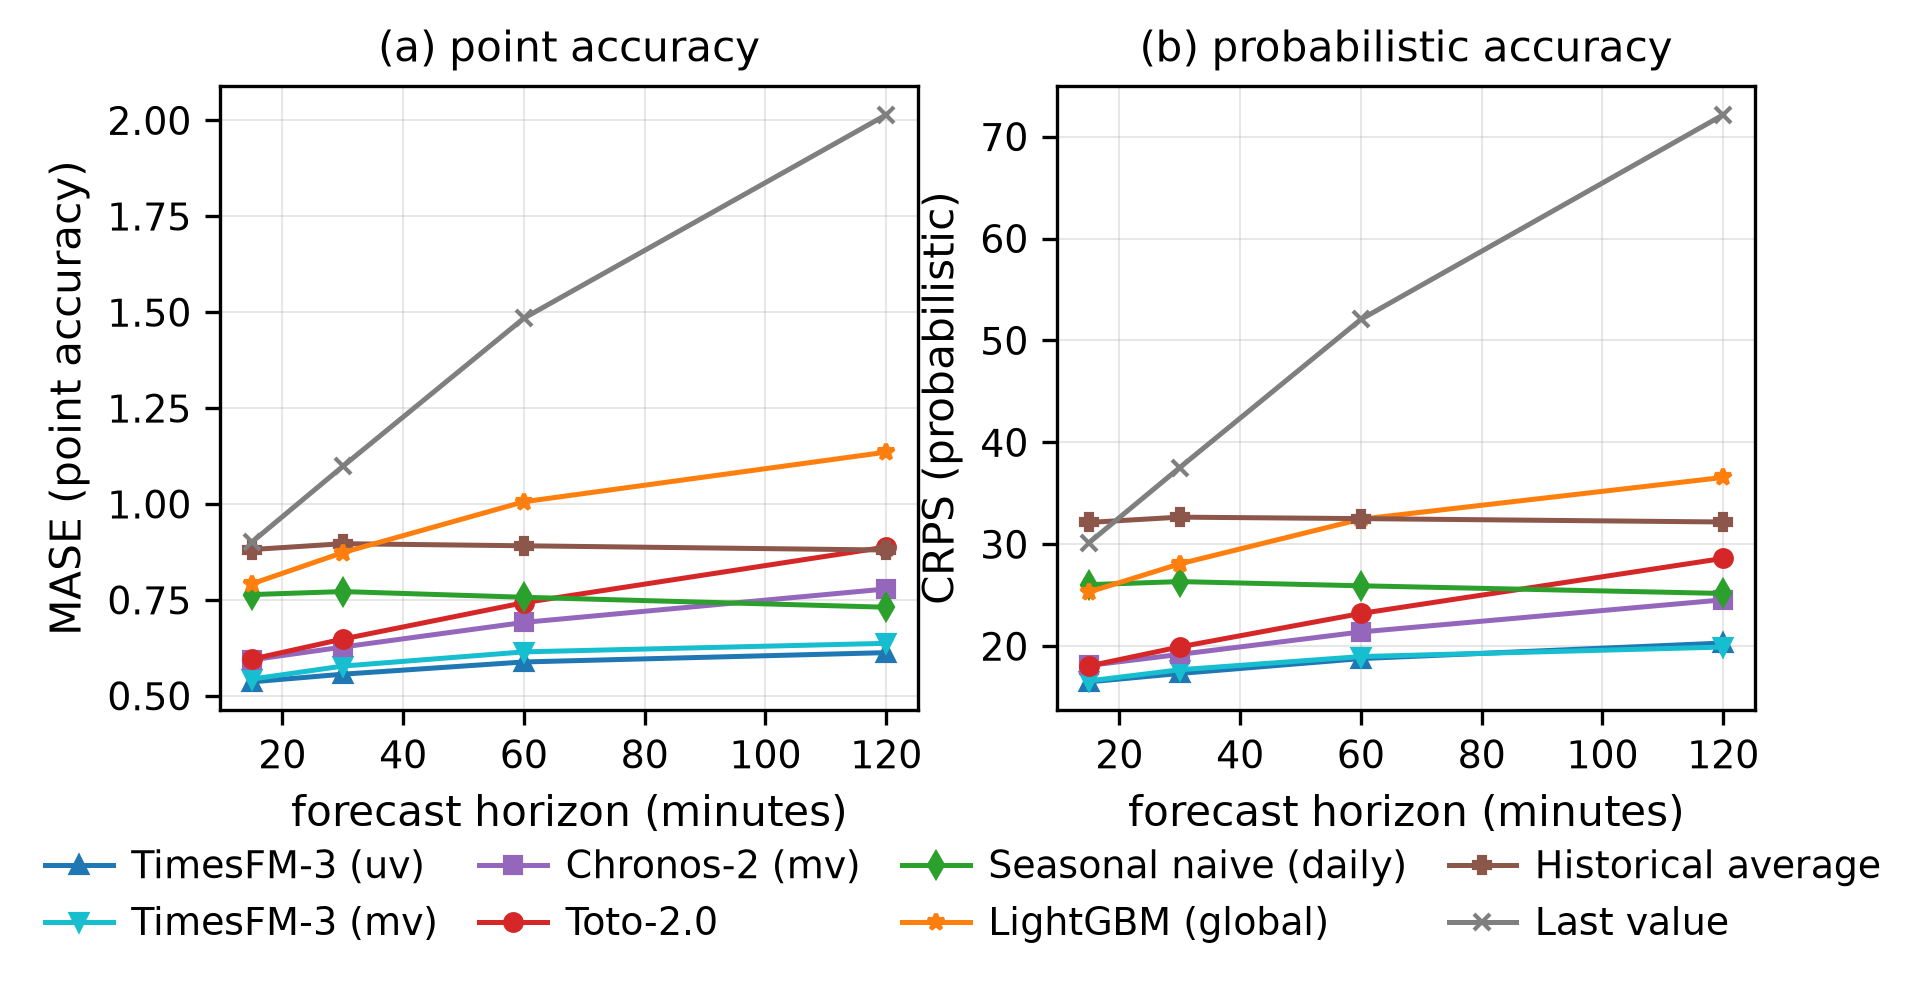
\includegraphics[width=0.92\textwidth]{figures/point_vs_probabilistic.png}
\caption{Point and probabilistic accuracy on HZMetro, which agree here but need not. The ordering of methods is broadly preserved between MASE and CRPS, with one exception worth noting: Chronos-2 and Toto-2.0 trail the two TimesFM-3 configurations by more on MASE than on CRPS, because their wider intervals are penalised less by a score that rewards honest spread than by one that only reads the median.}
\label{fig:pointprob}
\end{figure}

\subsection{H4: topology-blindness, measured and repaired}

Table~\ref{tab:recon} quantifies the motivating claim of the paper on the simulated museum, the only site reporting both sides of~\eqref{eq:conservation}. Raw foundation model forecasts violate the continuity equation by \num{1.05} persons per node per interval. In a house museum gallery whose typical occupancy is a handful of people this is not a rounding error: it means the forecast asserts that people appear in, or vanish from, rooms.

\begin{table}[htbp]
\centering
\caption{Reconciliation on the simulated museum, \new{at two operating points}, scored separately for each of two forecasters and computed offline from stored quantile forecasts. Residual is the mean absolute conservation violation and bound violation the total capacity and non-negativity violation, both in persons. \new{Peak error is the mean absolute error in the predicted maximum occupancy over the horizon\rev{, an error of magnitude that does not measure whether a threshold crossing is detected; Table~\ref{tab:risk} reports event detection separately}.} Solve time is the median in milliseconds. \new{The \emph{unbounded uncertainty} arm is new in this revision and uses the proposed diagonal $\bOm$ with the box removed, which is what makes the decomposition~\eqref{eq:decomposition} identifiable.}}
\label{tab:recon}
\footnotesize
\setlength{\tabcolsep}{5pt}
\begin{tabular}{lrrrrrr}
\toprule
Reconciler & Residual & Bound & MAE & CRPS & \new{Peak error} & Solve \\
\midrule
\multicolumn{7}{l}{\emph{\new{(a) Baseline configuration, \num{300} origins, capacity binding on \SI{2.7}{\percent} of room-steps}}}\\
None (raw)              & \num{1.055} & \num{0.006} & 0.3495 & 0.2687 & 1.298 & n/a \\
MinT (shrink)           & \num{<1e-9} & \num{2.062} & 0.3516 & 0.2719 & 1.258 & \num{<0.1} \\
\new{Unbounded uncertainty} & \num{<1e-9} & \num{1.414} & 0.3485 & 0.2700 & 1.223 & 2.6 \\
Uniform weight          & \num{<1e-9} & \num{0.000} & 0.3506 & 0.2717 & 1.250 & 6.1 \\
\textbf{Proposed}       & \num{<1e-9} & \num{0.000} & \best{0.3475} & \best{0.2697} & \best{1.217} & 6.2 \\
\midrule
\multicolumn{7}{l}{\emph{\new{(b) Crowded configuration, capacity binding on \SI{8.0}{\percent} of room-steps}}}\\
None (raw)              & \num{0.960} & \num{0.451} & 0.3654 & 0.2914 & 1.113 & n/a \\
MinT (shrink)           & \num{<1e-9} & \num{2.944} & 0.3676 & 0.2948 & 1.090 & \num{<0.1} \\
\new{Unbounded uncertainty} & \num{<1e-9} & \num{2.377} & 0.3652 & 0.2931 & 1.076 & 2.6 \\
Uniform weight          & \num{<1e-9} & \num{0.000} & 0.3661 & 0.2943 & 1.081 & 8.2 \\
\textbf{Proposed}       & \num{<1e-9} & \num{0.000} & \best{0.3633} & \best{0.2926} & \best{\rev{1.068}} & 7.2 \\
\bottomrule
\end{tabular}
\end{table}

All \new{four} reconcilers drive the conservation residual to solver tolerance, as Theorem~\ref{thm:unique} guarantees. The separation is in what they break on the way. MinT, which enforces the equalities by the \new{affine} map of Proposition~\ref{prop:mint} and has no representation of the box, introduces \new{\num{2.06}} persons of capacity and sign violation per origin. This is exactly the failure Proposition~\ref{prop:mint} predicts, and it is a consequential one: a reconciler that removes one class of physical impossibility by creating another has not delivered an admissible forecast. Both constrained projections leave the box exactly satisfied. Figure~\ref{fig:recon} shows the three criteria side by side; the proposed method is the only one that is not in the wrong on any of them. Hypothesis~\ref{hyp:coherence} is supported.

\new{\paragraph{The violation follows the missing box, not the choice of weights.} The new unbounded uncertainty arm settles this. It carries the proposed diagonal $\bOm$ and no box, and it violates the bounds by \num{1.41} persons, between MinT's \num{2.06} and the constrained arms' exact zero. Had the violation been an artefact of MinT's shrunk covariance rather than of its missing inequalities, this arm would have been clean. It is not, which confirms that the box is doing the work the paper attributes to it.}

\new{\paragraph{A crowded building, where the constraints actually bind.} A reviewer objected that a reconciliation result measured where the constraints are nearly inactive says little, noting that the raw bound violation in the submitted table was only \num{0.006} persons, so the box was essentially never active and the method's central feature was untested. The objection is correct and panel (b) answers it. We built a second configuration of the same floor plan with the same room capacities and doorway throughputs, raising the arrival rate from \num{1.6} to \num{7.0} visitors per minute at peak, adding a midday coach party on weekdays and lengthening dwell. Capacity then binds on \SI{8.0}{\percent} of room-steps against \SI{2.7}{\percent} in the baseline, and at the entrance specifically on \SI{20.5}{\percent} of steps against \SI{1.4}{\percent}. The raw bound violation rises by a factor of \num{75}, from \num{0.006} to \num{0.451} persons per origin, and MinT's violation rises from \num{2.06} to \num{2.94}. The qualitative conclusion is unchanged and the quantitative stakes are much higher: in the regime the method exists for, an unboxed reconciler asserts nearly three persons per origin of physically impossible occupancy, and a boxed one asserts none. This is the clearest evidence in the paper for the inequality constraints, and it required building the crowded configuration to obtain.}

\begin{figure}[htbp]
\centering
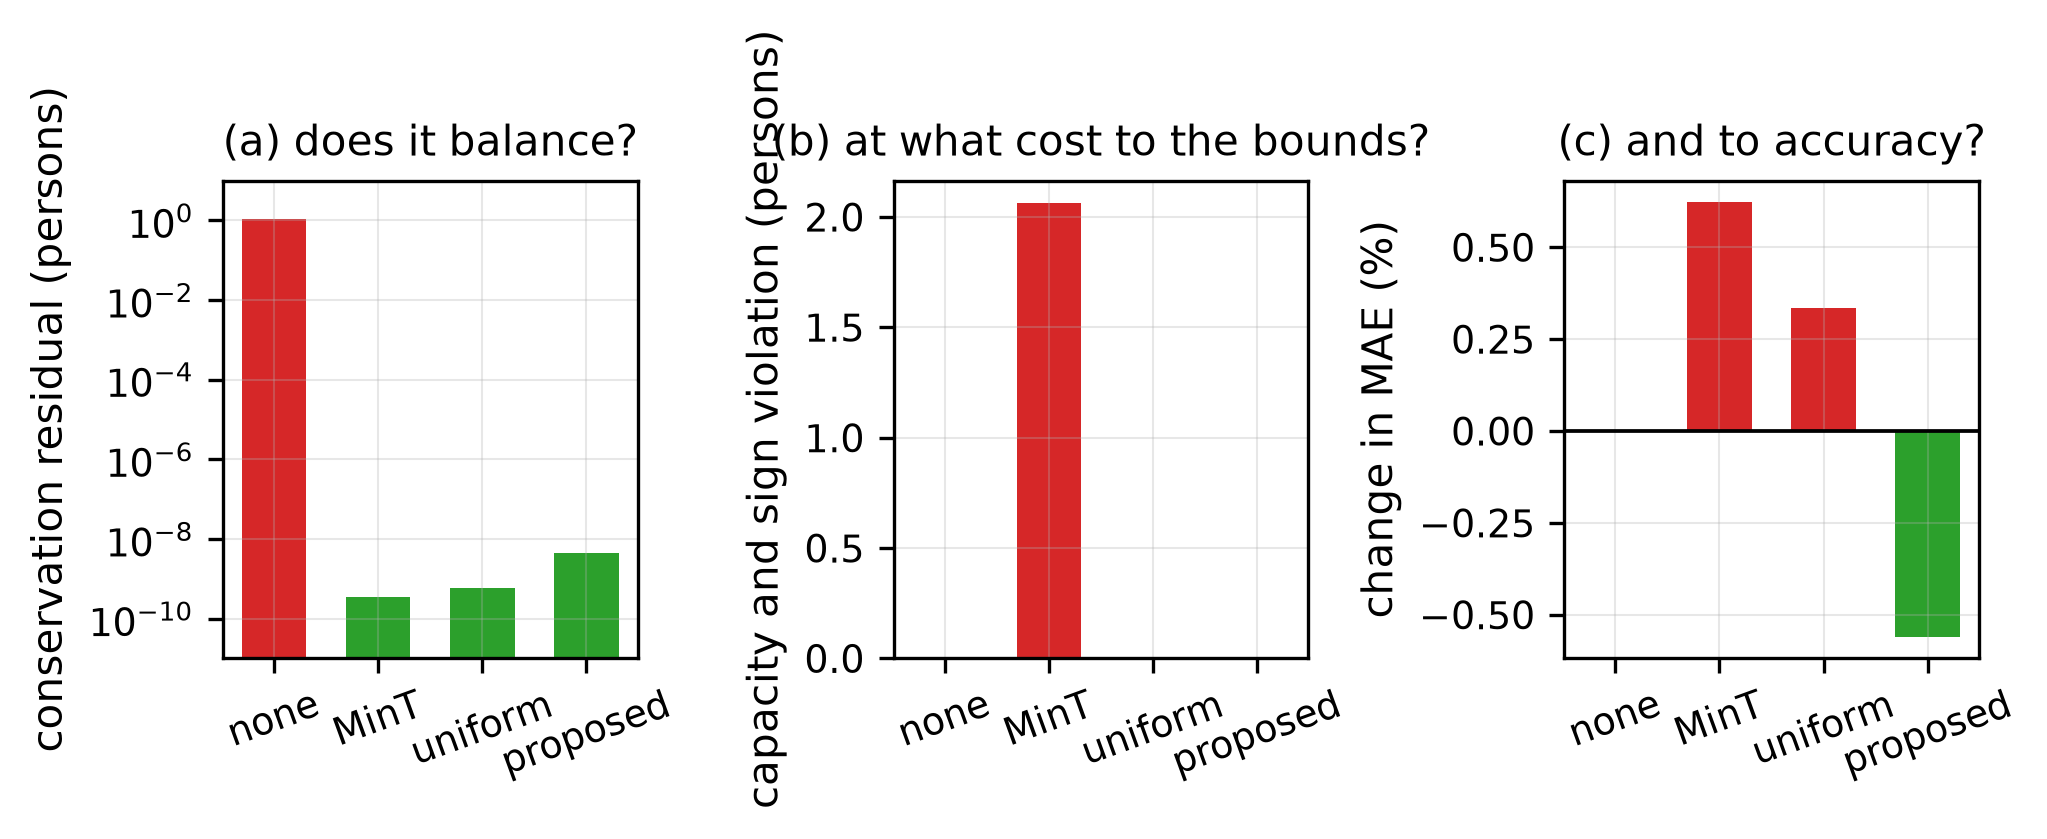
\includegraphics[width=0.95\textwidth]{figures/reconciliation.png}
\caption{Reconciliation must win on three criteria at once. (a) Every reconciler restores conservation. (b) Only MinT breaks the capacity and non-negativity constraints, as Proposition~\ref{prop:mint} predicts, because it has no representation of them. (c) Only the uncertainty-weighted projection improves point accuracy; uniform weighting enforces the same constraints and still degrades it. Green marks the desirable outcome.}
\label{fig:recon}
\end{figure}

\subsection{H5: the uncertainty weighting is what makes it pay}

\new{Table~\ref{tab:ablation} isolates the two design decisions this method rests on, using the decomposition~\eqref{eq:decomposition} that the new unbounded arm makes possible. Each row is a paired comparison over identical origins, so the two arms differ in exactly one respect, and each effect carries a moving-block bootstrap interval alongside its $p$-value because a reviewer asked for intervals on the mean paired change and because, as explained below, the mean and the median here disagree in sign.}

\new{\begin{table}[htbp]
\centering
\caption{\new{What the weighting does and what the box does, as separately identified effects. Each entry is the change in MAE of the first arm relative to the second, as a percentage of the second arm's MAE, so negative favours the first arm. The interval is a \SI{95}{\percent} moving-block bootstrap interval for the mean with blocks of ten consecutive origins; the $p$-value is \rev{from a paired Wilcoxon signed-rank test, whose null hypothesis is symmetry of the paired differences about zero. On differences as skewed as these it is a test of neither the mean nor the median, and Table~\ref{tab:typical} gives a direct test of each. The signed-rank test is one-sided, in the direction of the stated hypothesis, in the three ablation blocks and two-sided in the last block, which the earlier caption did not say.} ``Worse'' is the fraction of origins the first arm makes worse\rev{, a paired difference smaller than \num{e-12} persons in absolute value being counted as a tie. One entry is corrected on that account: the unbounded arm is worse than MinT on \SI{11}{\percent} of origins for TimesFM-3, not \SI{20}{\percent}, the earlier figure having counted \num{28} origins whose difference was floating-point noise}.}}
\label{tab:ablation}
\footnotesize
\setlength{\tabcolsep}{5pt}
\begin{tabular}{llrlrrr}
\toprule
Comparison & Forecaster & mean \% & \SI{95}{\percent} CI & median \% & $p$ & worse \\
\midrule
\multicolumn{7}{l}{\emph{Effect of the uncertainty weighting, box held on}}\\
Proposed vs uniform & TimesFM-3 & $-1.20$ & $[-1.70,-0.77]$ & $-0.01$ & \num{7.1e-23} & \SI{12}{\percent} \\
Proposed vs uniform & LightGBM  & $-0.56$ & $[-0.83,-0.29]$ & $-0.00$ & \num{4.7e-08} & \SI{9}{\percent} \\
\midrule
\multicolumn{7}{l}{\emph{Effect of the box, proposed weighting held on}}\\
Proposed vs unbounded & TimesFM-3 & $-0.28$ & $[-0.44,-0.16]$ & $-0.02$ & \num{6.2e-44} & \SI{2}{\percent} \\
Proposed vs unbounded & LightGBM  & $-0.30$ & $[-0.39,-0.23]$ & $-0.00$ & \num{1.3e-13} & \SI{4}{\percent} \\
\midrule
\multicolumn{7}{l}{\emph{Effect of the weighting matrix, equalities only, versus MinT}}\\
Unbounded vs MinT & TimesFM-3 & $-1.07$ & $[-1.49,-0.69]$ & $-0.01$ & \num{1.4e-25} & \rev{\SI{11}{\percent}} \\
Unbounded vs MinT & LightGBM  & $-0.69$ & $[-0.94,-0.46]$ & $-0.00$ & \num{9.1e-09} & \SI{8}{\percent} \\
\midrule
\multicolumn{7}{l}{\emph{For comparison: the whole layer against the raw forecast}}\\
Proposed vs raw & TimesFM-3 & $-0.98$ & $[-1.41,-0.61]$ & $+0.01$ & \num{1.8e-1} & \SI{70}{\percent} \\
Proposed vs raw & LightGBM  & $-0.10$ & $[-0.39,+0.19]$ & $+0.00$ & \num{1.1e-1} & \SI{15}{\percent} \\
\bottomrule
\end{tabular}
\end{table}}

\new{Both design decisions are confirmed, and the comparison that the submitted paper should have made is the middle block. Holding the weighting fixed and removing only the box costs \SI{0.28}{\percent} and \SI{0.30}{\percent} of MAE for the two forecasters. Holding the constraint set at equalities only and replacing MinT's shrunk covariance with the proposed diagonal $\bOm$ gains \SI{1.07}{\percent} and \SI{0.69}{\percent}. The weighting matrix is therefore the larger of the two effects by a factor of roughly three, and the submitted paper's attribution of the whole proposed-versus-MinT difference to the box was wrong in emphasis as well as in logic. Both effects are in the claimed direction, both are highly significant, and both are small in absolute terms. Hypothesis~\ref{hyp:weights} is supported.}

\new{\paragraph{The whole layer against the raw forecast is a weaker result, and we separate it.} A reviewer asked that the strong feasibility finding be kept apart from the limited accuracy evidence, noting the \SI{0.98}{\percent} improvement for TimesFM-3 at $p=\num{0.18}$. The last block of Table~\ref{tab:ablation} is that separation. Against the raw forecast the mean improvement is \SI{0.98}{\percent} for TimesFM-3 and \SI{0.10}{\percent} for LightGBM, and neither is significant by a signed-rank test. \rev{A reviewer of this revision pointed out that the two statistics reported for TimesFM-3 appear to conflict, an interval for the mean of $[-1.41,-0.61]$ that excludes zero beside a signed-rank $p$-value of \num{0.18}, and asked that the mean improvement be distinguished from the improvement at a typical origin. The two statistics do not conflict, because they answer different questions, but the earlier text did not say which question each answers and described the signed-rank test, incorrectly, as a statement about the median. Table~\ref{tab:typical} separates the questions and tests each directly.}}

\rev{\emph{The mean.} For TimesFM-3 the mean paired change in MAE is $-\SI{0.98}{\percent}$ with a moving-block bootstrap interval of $[-1.41,-0.61]$ on the baseline configuration and $-\SI{1.25}{\percent}$ with $[-1.69,-0.82]$ on the crowded one. Both exclude zero, so a reduction in mean error is statistically established for this forecaster on the simulator. For LightGBM the mean change is $-\SI{0.10}{\percent}$ with $[-0.39,+0.19]$ and $+\SI{0.17}{\percent}$ with $[-0.21,+0.41]$, so no change in mean error is established in either direction.}

\rev{\emph{The typical origin.} For TimesFM-3 the median paired change is $+\SI{0.013}{\percent}$ of MAE, with a bootstrap interval of $[+0.011,+0.015]$ that also excludes zero, on the other side. The projection worsens \num{211} of the \num{300} origins and improves \num{89}, and an exact sign test rejects equal odds at $p=\num{1.4e-12}$. On the crowded configuration the median is $+\SI{0.006}{\percent}$ with $[+0.003,+0.007]$, and \num{179} origins worsen against \num{121}, $p=\num{9.7e-4}$. It is therefore established, and not merely suggested, that the typical origin is made worse, by an amount some two orders of magnitude smaller than the mean improvement. For LightGBM the median change is exactly zero, because the projection leaves the forecast unchanged to within \num{e-12} persons on \num{185} of \num{300} origins; among the \num{115} it changes, \num{69} improve and \num{46} worsen on the baseline configuration ($p=\num{0.040}$, uncorrected) and \num{59} against \num{65} on the crowded one ($p=\num{0.65}$).}

\rev{\emph{Why the signed-rank test rejects neither.} The paired differences for TimesFM-3 are strongly left-skewed, with sample skewness $-4.9$: many small positive differences and a minority of large negative ones. The signed-rank statistic sums the ranks of the positive differences and compares them with those of the negative ones. Here the positive differences are numerous and low-ranked and the negative ones few and high-ranked, the two sums nearly balance, and the test returns $p=\num{0.18}$. Its null hypothesis is symmetry about zero, which is false in a way the statistic happens not to detect, so its failure to reject is evidence neither that the mean is zero nor that the median is. We retain it in Table~\ref{tab:ablation} for continuity and draw no conclusion from it.}

\rev{\emph{Sensitivity to the block length.} The block of ten origins was chosen in advance and is not critical. The lag-one autocorrelation of the paired difference is $-0.09$ for TimesFM-3 and $-0.02$ for LightGBM on the baseline configuration, so there is little serial dependence for the blocks to absorb. The strong serial dependence reported in Section~\ref{sec:depend} belongs to a different quantity, the loss differential between two forecasters on the real datasets, and the corresponding sensitivity is reported there. Table~\ref{tab:block} repeats the intervals at block lengths of \num{1}, \num{5}, \num{10}, \num{20} and \num{40} origins, the first being the ordinary bootstrap that assumes independence. No conclusion changes: for TimesFM-3 the interval for the mean excludes zero and the interval for the median lies above zero at every length and at both operating points, and for LightGBM the interval for the mean contains zero at every length. The same holds for the six ablation intervals of Table~\ref{tab:ablation}, each of which excludes zero at every block length.}

\rev{The reason the ablations are overwhelmingly significant by every test while the comparison against the raw forecast divides in this way is that the raw forecast is already nearly coherent on most origins, with a mean residual of \num{1.05} persons concentrated in a minority of occasions. On most origins the projection has little to correct and the small move it makes costs slightly more than it gains; on a minority it corrects a large error. We state the results at the strengths the evidence supports. The layer delivers exact coherence and exact feasibility, which is a guarantee and not an estimate. For TimesFM-3 it reduces the mean error by about one percent, which is statistically established on the simulator, while making the typical origin worse by about one hundredth of one percent, which is also established. For LightGBM no effect on the mean is established. The internal design choices within the layer are established with high confidence.}

\rev{\begin{table}[htbp]
\centering
\revcolor
\caption{\rev{Mean and typical-origin effects, tested separately. Each row is a paired comparison over \num{300} origins and each entry a change in MAE as a percentage of the second arm's mean MAE, negative favouring the first arm. Intervals are \SI{95}{\percent} moving-block bootstrap intervals with blocks of ten origins and \num{4000} resamples, computed separately for the mean and for the median. The counts are origins improved, worsened and tied; the sign test is an exact two-sided binomial test of equal odds on the untied origins. The signed-rank $p$-value is given for comparison and is two-sided in every row; for the ablation rows it is therefore twice the one-sided value of Table~\ref{tab:ablation}.}}
\label{tab:typical}
\footnotesize
\setlength{\tabcolsep}{2.5pt}
\resizebox{\ifdim\width>\textwidth\textwidth\else\width\fi}{!}{%
\begin{tabular}{llrlrlrrr}
\toprule
Comparison & Forecaster & mean & \SI{95}{\percent} CI & median & \SI{95}{\percent} CI & impr.\,/\,wors.\,/\,tied & sign $p$ & rank $p$ \\
\midrule
\multicolumn{9}{l}{\emph{(a) Baseline configuration}}\\
Proposed vs raw & TimesFM-3 & $-0.98$ & $[-1.41,-0.61]$ & $+0.013$ & $[+0.011,+0.015]$ & 89 / 211 / 0 & \num{1.4e-12} & \num{1.8e-1} \\
Proposed vs raw & LightGBM  & $-0.10$ & $[-0.39,+0.19]$ & $0.000$ & $[0.000,0.000]$ & 69 / 46 / 185 & \num{4.0e-2} & \num{1.1e-1} \\
Proposed vs uniform & TimesFM-3 & $-1.20$ & $[-1.70,-0.77]$ & $-0.008$ & $[-0.012,-0.003]$ & 234 / 37 / 29 & \num{3.6e-36} & \num{1.4e-22} \\
Proposed vs uniform & LightGBM  & $-0.56$ & $[-0.83,-0.29]$ & $0.000$ & $[0.000,0.000]$ & 89 / 26 / 185 & \num{3.0e-9} & \num{9.4e-8} \\
Proposed vs unbounded & TimesFM-3 & $-0.28$ & $[-0.44,-0.16]$ & $-0.019$ & $[-0.020,-0.017]$ & 293 / 7 / 0 & \num{4.1e-77} & \num{1.2e-43} \\
Proposed vs unbounded & LightGBM  & $-0.30$ & $[-0.39,-0.23]$ & $0.000$ & $[0.000,0.000]$ & 102 / 13 / 185 & \num{2.7e-18} & \num{2.5e-13} \\
Unbounded vs MinT & TimesFM-3 & $-1.07$ & $[-1.49,-0.69]$ & $-0.010$ & $[-0.015,-0.004]$ & 238 / 33 / 29 & \num{1.8e-39} & \num{2.9e-25} \\
Unbounded vs MinT & LightGBM  & $-0.69$ & $[-0.94,-0.46]$ & $0.000$ & $[0.000,0.000]$ & 91 / 24 / 185 & \num{2.3e-10} & \num{1.8e-8} \\
\midrule
\multicolumn{9}{l}{\emph{(b) Crowded configuration}}\\
Proposed vs raw & TimesFM-3 & $-1.25$ & $[-1.69,-0.82]$ & $+0.006$ & $[+0.003,+0.007]$ & 121 / 179 / 0 & \num{9.7e-4} & \num{4.7e-1} \\
Proposed vs raw & LightGBM  & $+0.17$ & $[-0.21,+0.41]$ & $0.000$ & $[0.000,0.000]$ & 59 / 65 / 176 & \num{6.5e-1} & \num{3.0e-1} \\
\bottomrule
\end{tabular}}
\end{table}}

\rev{\begin{table}[htbp]
\centering
\revcolor
\caption{\rev{Sensitivity of the bootstrap intervals to the block length, for the proposed projection against the raw forecast. Entries are \SI{95}{\percent} intervals for the paired change in MAE, in percent. A block of one origin is the ordinary bootstrap; ten is the length used elsewhere in the paper. The median interval for LightGBM is $[0,0]$ at every length and is omitted.}}
\label{tab:block}
\footnotesize
\setlength{\tabcolsep}{2.5pt}
\resizebox{\ifdim\width>\textwidth\textwidth\else\width\fi}{!}{%
\begin{tabular}{llccccc}
\toprule
& & \multicolumn{5}{c}{block length, in origins} \\
\cmidrule(lr){3-7}
Configuration & Quantity & 1 & 5 & 10 & 20 & 40 \\
\midrule
Baseline & TimesFM-3, mean   & $[-1.48,-0.54]$ & $[-1.41,-0.59]$ & $[-1.41,-0.61]$ & $[-1.33,-0.61]$ & $[-1.32,-0.62]$ \\
Baseline & TimesFM-3, median & $[+0.010,+0.015]$ & $[+0.011,+0.015]$ & $[+0.011,+0.015]$ & $[+0.011,+0.015]$ & $[+0.011,+0.015]$ \\
Baseline & LightGBM, mean    & $[-0.43,+0.22]$ & $[-0.43,+0.23]$ & $[-0.39,+0.19]$ & $[-0.33,+0.12]$ & $[-0.32,+0.15]$ \\
\midrule
Crowded  & TimesFM-3, mean   & $[-1.81,-0.75]$ & $[-1.76,-0.78]$ & $[-1.69,-0.82]$ & $[-1.62,-0.83]$ & $[-1.51,-0.89]$ \\
Crowded  & TimesFM-3, median & $[+0.004,+0.007]$ & $[+0.002,+0.007]$ & $[+0.003,+0.007]$ & $[+0.003,+0.007]$ & $[+0.004,+0.007]$ \\
Crowded  & LightGBM, mean    & $[-0.19,+0.52]$ & $[-0.17,+0.46]$ & $[-0.21,+0.41]$ & $[-0.19,+0.31]$ & $[-0.16,+0.26]$ \\
\bottomrule
\end{tabular}}
\end{table}}

\rev{\paragraph{Risk-sensitive evaluation: what is shown and what is not.}
\label{sec:risk}
A reviewer of the first revision observed that roughly \SI{70}{\percent} of origins become slightly worse under the proposed projection and asked whether a risk-sensitive metric tells a different story. The earlier version of this paragraph answered with the peak error alone and concluded that the gain lands where a crowd-protection rule needs it. A reviewer of this revision objected that a lower average peak error does not by itself imply better identification of unsafe conditions, and noted that the high-occupancy error and the Brier score to which our response had referred were absent from the manuscript. Both points are correct. The two quantities had been computed and logged but not printed. Table~\ref{tab:risk} now reports them with the definitions of Section~\ref{sec:metrics}, and they do not support the conclusion that the earlier paragraph drew.}

\rev{\emph{Sample.} Each configuration scores \num{300} origins for each of two forecasters, and each origin contributes \num{8} rooms over \num{60} forecast steps, which is \num{144000} room-steps per forecaster. In the baseline configuration \num{5914} of these, \SI{4.1}{\percent}, have observed occupancy at or above \SI{80}{\percent} of capacity, spread over \num{82} origins, and \num{3316}, \SI{2.3}{\percent}, are at capacity, in \num{75} origins. In the crowded configuration the counts are \num{15307}, \SI{10.6}{\percent}, in \num{103} origins and \num{11460}, \SI{8.0}{\percent}, in \num{99} origins. Observed occupancy never exceeds capacity in the simulator, so the second event is a full room.}

\rev{\emph{Peak error.} The proposed projection reduces the mean absolute error of the predicted maximum occupancy from \num{1.298} to \num{1.217} persons on the baseline configuration, a reduction of \SI{6.3}{\percent}, and from \num{1.113} to \num{1.068} on the crowded one, a reduction of \SI{4.0}{\percent}. The paired reduction is \num{0.133} persons for LightGBM and \num{0.030} for TimesFM-3 on the baseline configuration and \num{0.057} and \num{0.032} on the crowded one, and all four block-bootstrap intervals exclude zero. This is the one risk-related effect that is statistically established, and it is a statement about the magnitude of the predicted peak. It says nothing about whether the peak is predicted at the right time, in the right room, or on the right side of a threshold.}

\rev{\emph{Error at high occupancy.} Restricted to the room-steps at or above \SI{80}{\percent} of capacity, the evidence is mixed. Averaged over origins the error moves from \num{4.319} to \num{4.280} persons on the baseline configuration and from \num{2.827} to \num{2.849} on the crowded one, an improvement and a deterioration; pooled over room-steps it moves from \num{3.408} to \num{3.350} and from \num{1.855} to \num{1.828}, two improvements. Of the four paired intervals, two exclude zero in the favourable direction, two contain zero, and one point estimate is unfavourable. The changes are between one and three percent of an error of \num{2.5} to \num{4.7} persons. An improvement in error at high occupancy is therefore not established.}

\rev{\emph{Detection of near-capacity and at-capacity conditions.} This is the quantity the reviewer's objection concerns, and here the projection changes very little. For the near-capacity event the hit rate moves from \SI{43.7}{\percent} to \SI{45.0}{\percent} on the baseline configuration and from \SI{80.1}{\percent} to \SI{80.6}{\percent} on the crowded one, with false alarms rising from \num{2095} to \num{2219} and from \num{3643} to \num{3658}. For the at-capacity event the hit rate moves from \SI{39.1}{\percent} to \SI{39.4}{\percent} and from \SI{68.4}{\percent} to \SI{68.6}{\percent}, with false alarms falling from \num{512} to \num{469} and from \num{2407} to \num{2312}. The Brier scores change in the fourth decimal place. Of the eight paired intervals for the change in Brier score, four exclude zero, all in the favourable direction, with relative reductions between \SI{0.7}{\percent} and \SI{1.8}{\percent}; the other four contain zero. A forecast that misses six in ten full-room room-steps on the baseline configuration before the projection misses six in ten after it. We conclude that reconciliation does not materially improve the identification of unsafe conditions in these experiments, and where a difference is detectable it is too small to matter operationally.}

\rev{\emph{A threshold rule we report and do not rely on.} Our response to the first revision referred to a Brier score for capacity exceedance. That score was computed with the strict rule $\tau_v = \theta_v = c_v$, under which a forecast predicts a full room only if it is numerically at or above capacity. Under that rule the projection appears to make detection substantially worse: the hit rate falls from \SI{16.2}{\percent} to \SI{11.7}{\percent} and from \SI{29.8}{\percent} to \SI{17.4}{\percent}, and the Brier score rises from \num{0.0194} to \num{0.0207} and from \num{0.0565} to \num{0.0672}. We print this because it is the score that was logged, and we rely on it in neither direction, because for a box-constrained forecast it is not a numerically well-defined quantity. The projection places every forecast that would exceed capacity on the bound, and the solver returns the bound only to within its tolerance of \num{e-7}, so whether the strict inequality holds is decided by the last digits of the solution. The evidence is direct. Solving the identical problems from a warm start instead of a cold start changes the MAE by less than \num{e-6} persons at every origin, and changes the number of strict-rule hits from \num{3991} to \num{4510} on the crowded configuration and from \num{777} to \num{782} on the baseline one, while every count under the half-person rule and under the near-capacity rule is identical to the last digit. This is why Section~\ref{sec:metrics} defines the at-capacity forecast event with a margin of half a person, and why the earlier reference to an exceedance score should not have been made without it.}

\rev{\emph{Three levels of claim.} The evidence separates three statements that the earlier text ran together. The first is \emph{average accuracy}: the projection reduces the mean error of TimesFM-3 by about one percent and leaves that of LightGBM unchanged, as established above. The second is \emph{risk-sensitive prediction}: the projection reduces the error in the magnitude of the predicted peak, which is established, and does not materially change the error at high occupancy or the detection of near-capacity and full-room conditions. The third is \emph{operational decision benefit}, meaning that an operator acting on the reconciled forecast would take better decisions, with adequate lead time and at an acceptable rate of false alarms. That was not evaluated at all: no decision rule was run, no lead time was measured and no cost was assigned to a missed event or a false alarm, since the decision-utility study of our original design remains unrun (Section~\ref{sec:limits}). We therefore withdraw the earlier statements that the gain lands on the origins the system exists to get right and that the peak result is operationally stronger than the MAE result. What the layer provides on the present evidence is a feasibility guarantee, a small and established reduction in mean error for one forecaster, and a more accurate predicted peak magnitude.}

\rev{\begin{table}[htbp]
\centering
\revcolor
\caption{\rev{Risk-sensitive quantities for the raw forecast and the proposed projection on the simulated museum, with the definitions of Section~\ref{sec:metrics}. Panel (a) pools the two forecasters: \num{600} origins and \num{288000} room-steps per configuration. The numbers of events are room-steps on which the outcome event occurs, over both forecasters. Hit rate is the share of events for which the forecast event also occurs; false alarms are room-steps where the forecast event occurs and the outcome event does not. Panel (b) gives the paired change, proposed minus raw, for each forecaster with a \SI{95}{\percent} moving-block bootstrap interval (blocks of ten origins); negative is an improvement, and Brier changes are in units of \num{e-3}. The high-occupancy rows of panel (b) use the \num{82} and \num{103} origins that contain a high-occupancy room-step. The strict rule is reported for transparency and is not numerically stable, as explained in the text.}}
\label{tab:risk}
\scriptsize
\setlength{\tabcolsep}{4pt}
\begin{tabular}{lcccc}
\toprule
& \multicolumn{2}{c}{Baseline configuration} & \multicolumn{2}{c}{Crowded configuration} \\
\cmidrule(lr){2-3}\cmidrule(lr){4-5}
\emph{(a) Level} & raw & proposed & raw & proposed \\
\midrule
Peak error, persons                         & 1.298 & 1.217 & 1.113 & 1.068 \\
High-occupancy MAE, mean over origins       & 4.319 & 4.280 & 2.827 & 2.849 \\
High-occupancy MAE, pooled over room-steps  & 3.408 & 3.350 & 1.855 & 1.828 \\
\midrule
\multicolumn{5}{l}{\emph{Near capacity, outcome and forecast at or above $0.8\,c_v$: \num{11828} and \num{30614} events}}\\
\quad Hit rate                              & \SI{43.7}{\percent} & \SI{45.0}{\percent} & \SI{80.1}{\percent} & \SI{80.6}{\percent} \\
\quad False alarms                          & \num{2095} & \num{2219} & \num{3643} & \num{3658} \\
\quad Brier score                           & 0.0304 & 0.0303 & 0.0338 & 0.0334 \\
\midrule
\multicolumn{5}{l}{\emph{At capacity, outcome at $c_v$, forecast at or above $c_v - 0.5$: \num{6632} and \num{22920} events}}\\
\quad Hit rate                              & \SI{39.1}{\percent} & \SI{39.4}{\percent} & \SI{68.4}{\percent} & \SI{68.6}{\percent} \\
\quad False alarms                          & \num{512} & \num{469} & \num{2407} & \num{2312} \\
\quad Brier score                           & 0.0158 & 0.0156 & 0.0335 & 0.0330 \\
\midrule
\multicolumn{5}{l}{\emph{At capacity, strict rule, forecast at or above $c_v$ (not numerically stable)}}\\
\quad Hit rate                              & \SI{16.2}{\percent} & \SI{11.7}{\percent} & \SI{29.8}{\percent} & \SI{17.4}{\percent} \\
\quad False alarms                          & \num{34} & \num{96} & \num{183} & \num{425} \\
\quad Brier score                           & 0.0194 & 0.0207 & 0.0565 & 0.0672 \\
\midrule
\emph{(b) Paired change, proposed minus raw} & \multicolumn{2}{c}{Baseline configuration} & \multicolumn{2}{c}{Crowded configuration} \\
\midrule
Peak error, LightGBM                        & \multicolumn{2}{c}{$-0.133\ [-0.155,-0.114]$} & \multicolumn{2}{c}{$-0.057\ [-0.090,-0.031]$} \\
Peak error, TimesFM-3                       & \multicolumn{2}{c}{$-0.030\ [-0.041,-0.020]$} & \multicolumn{2}{c}{$-0.032\ [-0.051,-0.017]$} \\
High-occupancy MAE, LightGBM                & \multicolumn{2}{c}{$-0.055\ [-0.090,-0.024]$} & \multicolumn{2}{c}{$+0.096\ [-0.038,+0.154]$} \\
High-occupancy MAE, TimesFM-3               & \multicolumn{2}{c}{$-0.023\ [-0.052,+0.024]$} & \multicolumn{2}{c}{$-0.051\ [-0.071,-0.037]$} \\
Near-capacity Brier, LightGBM               & \multicolumn{2}{c}{$-0.33\ [-0.65,+0.06]$} & \multicolumn{2}{c}{$-0.49\ [-0.92,-0.18]$} \\
Near-capacity Brier, TimesFM-3              & \multicolumn{2}{c}{$+0.13\ [-0.15,+0.43]$} & \multicolumn{2}{c}{$-0.47\ [-0.83,-0.15]$} \\
At-capacity Brier, LightGBM                 & \multicolumn{2}{c}{$-0.31\ [-0.72,+0.03]$} & \multicolumn{2}{c}{$-0.32\ [-0.71,+0.01]$} \\
At-capacity Brier, TimesFM-3                & \multicolumn{2}{c}{$-0.10\ [-0.20,-0.01]$} & \multicolumn{2}{c}{$-0.64\ [-1.21,-0.08]$} \\
\bottomrule
\end{tabular}
\end{table}}

Figure~\ref{fig:recondist} shows the distribution behind these means\new{, and it explains why the mean and the median disagree in sign}. For TimesFM-3 the proposed projection leaves \SI{70}{\percent} of origins very slightly worse and a minority of origins very much better, with a left tail reaching \SI{8}{\percent} improvement, so the mean is carried by the tail while the median \rev{barely moves}\new{, and is in fact very slightly positive}. The uniform arm has the opposite shape: an effect that is small, negative and almost universal. Reporting only the means would have hidden this. \rev{The statistical reading} is that uncertainty weighting is not a uniform small improvement but an intervention that occasionally matters a great deal, at origins where the forecast was badly wrong in a direction its own quantile spread had flagged.

\begin{figure}[htbp]
\centering
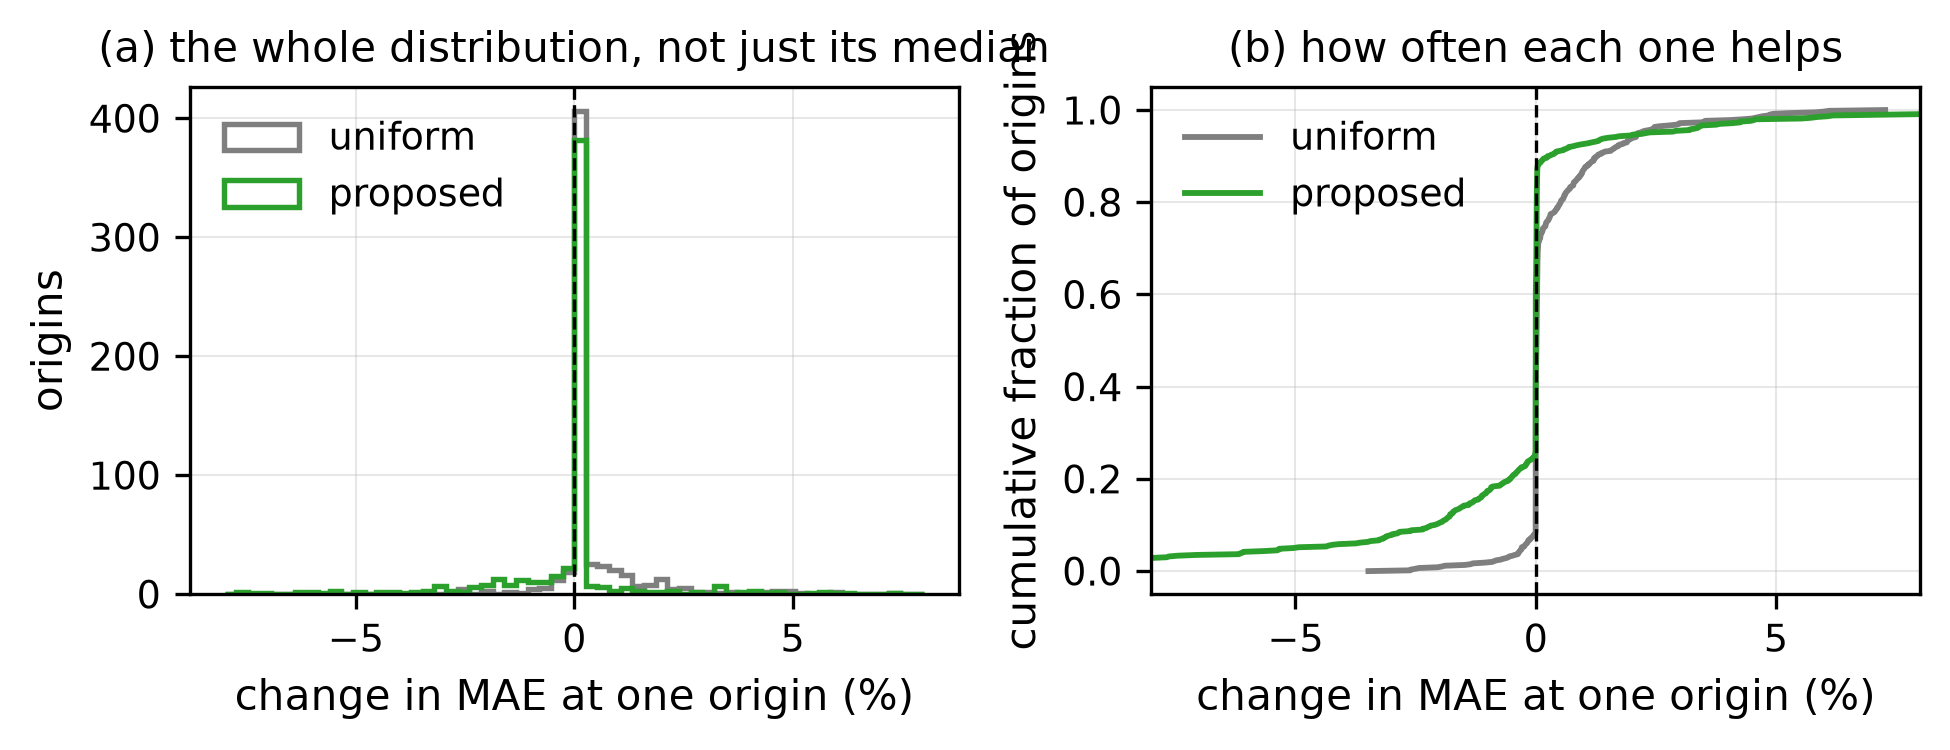
\includegraphics[width=0.92\textwidth]{figures/reconciliation_distribution.png}
\caption{Why a larger mean effect can carry a weaker $p$-value. (a) Per-origin change in MAE for the two weighting schemes; (b) the same as cumulative distributions. Uniform weighting shifts almost every origin slightly the wrong way. The proposed weighting leaves the median origin near zero and produces a heavy tail of large improvements, so its mean gain is real but is not a statement about the typical origin.}
\label{fig:recondist}
\end{figure}

The size of the point-accuracy gain is modest and we do not oversell it. Its importance is not the percentage but the sign, and the interpretation is precisely the one Corollary~\ref{cor:expected} anticipates. Theorem~\ref{thm:contraction} guarantees improvement in the $\bOm$-norm, not in MAE, so whether the guarantee survives the change of metric depends entirely on whether $\bOm$ points at the coordinates that were actually wrong. The uniform arm shows that when it does not, coherence is bought at a real cost in accuracy. The proposed arm shows that the quantile spread of a modern foundation model is informative enough about its own errors to convert that cost into a gain \rev{in the mean, though not at the typical origin (Table~\ref{tab:typical})}. We are not aware of prior direct evidence that a foundation model's predictive interval is useful as a reconciliation metric, and it is the practical reason the layer is worth adding rather than merely being defensible.

CRPS moves slightly the other way, from \num{0.2687} to \num{0.2697}. The shift strategy translates every quantile by the median correction and therefore holds interval widths fixed, so a shifted interval that is now correctly located may be marginally worse scored if the raw spread was already tuned to an incoherent median. We report this rather than selecting the strategy that hides it.

\subsection{\new{How incoherent are the non-median quantiles?}}
\label{sec:quantcoh}

\new{Section~\ref{sec:method} derives, in~\eqref{eq:shiftresidual}, that the shift strategy leaves a conservation residual of $\bA(\yhat^{\alpha}-\yhat^{0.5})$ at level $\alpha$. Table~\ref{tab:quantcoh} measures it, so that the withdrawn claim is replaced by a number rather than by an argument.}

\new{\begin{table}[htbp]
\centering
\caption{\new{Coherence level by level, on the simulated museum. Residual is the mean absolute conservation violation in persons and bound is the total capacity and sign violation. The shift strategy is exactly coherent and exactly feasible at the median and at no other level, as~\eqref{eq:shiftresidual} predicts. \rev{Per-quantile projection is reported twice: as the nine independent projections return it, where every level is coherent to solver tolerance and feasible but the levels cross, and after the monotone rearrangement that removes the crossings, which is what the implementation returns and what an earlier version of this table reported without saying so. Both cost nine times one solve. All rows are computed on the same \num{120} origin and forecaster pairs, \num{60} origins for each of two forecasters, on the baseline configuration.}}}
\label{tab:quantcoh}
\small
\begin{tabular}{lcccccccccc}
\toprule
& \multicolumn{9}{c}{quantile level $\alpha$} \\
\cmidrule(lr){2-10}
Strategy & 0.1 & 0.2 & 0.3 & 0.4 & 0.5 & 0.6 & 0.7 & 0.8 & 0.9 \\
\midrule
\multicolumn{10}{l}{\emph{Conservation residual}}\\
Shift        & 0.044 & 0.041 & 0.044 & 0.039 & \best{0.000} & 0.033 & 0.058 & 0.068 & 0.085 \\
\rev{Per quantile, as projected} & \rev{\best{0.000}} & \rev{\best{0.000}} & \rev{\best{0.000}} & \rev{\best{0.000}} & \rev{\best{0.000}} & \rev{\best{0.000}} & \rev{\best{0.000}} & \rev{\best{0.000}} & \rev{\best{0.000}} \\
\rev{Per quantile, rearranged} & 0.012 & 0.009 & 0.008 & 0.008 & 0.006 & 0.004 & 0.004 & 0.003 & 0.004 \\
\midrule
\multicolumn{10}{l}{\emph{Bound violation}}\\
Shift        & 9.832 & 6.238 & 4.347 & 2.179 & \best{0.000} & 0.132 & 0.390 & 1.285 & 6.656 \\
\rev{Per quantile, as projected} & \best{0.000} & \best{0.000} & \best{0.000} & \best{0.000} & \best{0.000} & \best{0.000} & \best{0.000} & \best{0.000} & \best{0.000} \\
\rev{Per quantile, rearranged} & \rev{\best{0.000}} & \rev{\best{0.000}} & \rev{\best{0.000}} & \rev{\best{0.000}} & \rev{\best{0.000}} & \rev{\best{0.000}} & \rev{\best{0.000}} & \rev{\best{0.000}} & \rev{\best{0.000}} \\
\midrule
\multicolumn{10}{l}{\rev{\emph{Share of coordinates moved by the rearrangement, in percent}}}\\
\rev{Per quantile, rearranged} & \rev{21.7} & \rev{21.0} & \rev{20.4} & \rev{20.3} & \rev{19.6} & \rev{17.9} & \rev{16.7} & \rev{13.4} & \rev{9.4} \\
\bottomrule
\end{tabular}
\end{table}}

\new{The measurement confirms the algebra and is more damaging to the submitted claim than the algebra alone suggests. Under the shift, the median is coherent to \num{2e-10} persons and every other level carries a residual between \num{0.033} and \num{0.085} persons, rising towards the tails exactly as~\eqref{eq:shiftresidual} requires, since the raw fan spreads furthest from its median there. The bound violations are the serious part: the \num{10}th percentile path violates the box by \num{9.83} persons per origin and the \num{90}th by \num{6.66}, because a common downward translation drives low quantiles of near-empty rooms below zero and a common upward one drives high quantiles of busy rooms above capacity. The submitted paper described this output as a coherent predictive distribution. It is a coherent median path wrapped in a fan that is neither coherent nor feasible, and the correct description is the one now given in Section~\ref{sec:method}.}

\rev{\paragraph{Why the per-quantile residual was not zero.} An earlier version of Table~\ref{tab:quantcoh} gave a single per-quantile row with residuals between \num{0.003} and \num{0.012} persons, including \num{0.006} at the median, and the accompanying text attributed them to solver tolerance accumulated over nine solves and stated that the crossing rate before any monotone repair was zero. A reviewer pointed out that the median residual needed explaining, since the shift and the per-quantile strategy project the same median and the shift leaves a residual of essentially zero. The reviewer's suspicion was justified, and both of our statements were wrong.}

\rev{The two strategies do solve the same problem at the median. Each calls the same routine on the same raw median, with the same weights $\bOm$, obtained from the same quantile spread by~\eqref{eq:sigma}, the same conservation equalities, the same box and the same solver settings. Before any further processing the two medians agree to within \num{4.2e-5} persons at every coordinate of every origin, and the per-quantile median has a mean absolute residual below \num{e-9} persons, like every other level: the mean residual at each of the nine levels is below \num{e-9} persons, and the largest residual in any single equation at any origin is \num{3.8e-6} persons. These are the magnitudes that the tolerances stated in Section~\ref{sec:method} imply, absolute and relative tolerances of \num{e-7} with solution polishing and a rejection threshold of \num{e-4}, and they are about seven orders of magnitude below the residuals in the earlier table. Solver tolerance was not the explanation.}

\rev{The explanation is the monotone rearrangement of Section~\ref{sec:method}. The nine independent projections do not preserve the order of the levels: \SI{11.3}{\percent} of adjacent quantile pairs cross, and \SI{73}{\percent} of the origin and forecaster pairs contain at least one crossing. The crossing rate of zero that we reported was measured after the rearrangement, where it is zero by construction, and the statement that it was measured before any repair was an error in the analysis script, which we have corrected. The rearrangement sorts the nine values of each coordinate and thereby moves between \SI{9.4}{\percent} and \SI{21.7}{\percent} of the coordinates of a level to a different level, including \SI{19.6}{\percent} of the coordinates of the median. Each rearranged path is then a mixture, coordinate by coordinate, of several paths that were each coherent, and such a mixture is not coherent, because the conservation constraint couples coordinates within a path. The residuals of \num{0.003} to \num{0.012} persons are produced entirely by this step. The rearranged median differs from the projected median by up to \num{2.2} persons at a single coordinate. The bound violation stays at zero through the rearrangement, since every level is projected onto the same box and a coordinatewise sort of values inside an interval remains inside it.}

\rev{Three consequences follow. The per-quantile strategy as implemented does not return a coherent median, whereas the shift does; under the per-quantile strategy the exactly coherent median is available only if the output is left unsorted. The reduction in residual relative to the shift at the non-median levels, by a factor of between \num{4} and \num{20}, is real for the rearranged output, and the unsorted output is exactly coherent at every level at the price of crossing quantiles. Neither is a coherent joint distribution: the unsorted paths are not the quantiles of any law, because they cross, and the rearranged paths are ordered but only approximately coherent, and in neither case is there a joint law over the series of which they are the marginal quantiles. The distinction between marginally feasible quantile paths and a coherent joint predictive distribution, drawn in Section~\ref{sec:method}, is therefore sharper than the earlier text made it: marginal coherence and monotonicity cannot both be obtained by projecting quantiles independently.}

\new{We did not adopt \rev{the per-quantile strategy} as the default for the reason given in Section~\ref{sec:method}\rev{, which the measurement reinforces}. We report the option and its cost, and recommend the shift with the narrower claim attached\rev{: an exactly coherent and feasible median path, with non-median levels that are ordered, mildly incoherent and not guaranteed to respect the box}.}

\subsection{\new{Does the Gaussian reading of the interval matter?}}
\label{sec:sigma}

\new{A reviewer noted that~\eqref{eq:sigma} converts an eighty percent interval into a standard deviation through a Gaussian quantile while occupancy counts are sparse, discrete and certainly not Gaussian, and asked whether the assumption is necessary and how sensitive the result is to the choice of interval. The answer is that it is not necessary, and the reason is structural rather than empirical.}

\new{The projection~\eqref{eq:qp} minimises a quadratic form in which only the \emph{relative} weights matter: replacing $\bOm$ by $\lambda\bOm$ for any $\lambda>0$ scales the objective without moving its argmin. The Gaussian constant $2z_{0.9} \approx 2.5631$ is exactly such a scalar, so it divides out of the solution entirely, and the Gaussian reading of the interval has no effect whatsoever on the projected point. We make this exact in the implementation by normalising $\bOm$ to unit mean diagonal before the solve, which is a no-op mathematically but is necessary numerically, because a solver compares its residual against an absolute tolerance and would otherwise solve the same problem to different accuracies depending on the units in which $\sigma$ happened to be expressed. With that normalisation in place, dividing the \SI{80}{\percent} width by \num{2.5631} and not dividing it at all give bit-identical reconciled forecasts, which we assert as a unit test rather than only observing.}

\new{What could matter is not the constant but the \emph{shape} of the map, meaning which part of the fan is read. Table~\ref{tab:sigma} varies that. Reading the central \SI{60}{\percent} interval instead of the \SI{80}{\percent} changes the MAE after reconciliation from \num{0.3176} to \num{0.3181}, and reading the central \SI{40}{\percent} changes it to \num{0.3190}: degradations of \SI{0.15}{\percent} and \SI{0.43}{\percent}. Individual coordinates move more than that, by up to \num{1.9} persons, so the choice is not vacuous, but the aggregate effect is an order of magnitude smaller than the effects the method is claimed to produce. The projection is therefore robust to the distributional assumption in the only sense that matters, and we no longer rest any claim on normality.}

\new{\begin{table}[htbp]
\centering
\caption{\new{Sensitivity of the projection to how the predictive spread is read, on \num{120} origin-forecaster pairs of the simulated museum. The first two rows differ by the multiplicative constant \num{2.5631} alone and are identical to machine precision, which is the scale invariance of the objective. The last two read a narrower interval and therefore change the relative weights. The final column reports the share of coordinates whose spread is clipped by the floor $\varepsilon$, which is high because many galleries are shut or empty for much of the day and the models correctly predict them with near-zero spread.}}
\label{tab:sigma}
\small
\begin{tabular}{llccc}
\toprule
Mapping & $\sigma_i$ from & MAE after & max coordinate shift & at floor \\
\midrule
Gaussian \SI{80}{\percent} (published) & $(q_{90}-q_{10})/2.5631$ & 0.31760 & ref. & \SI{63.6}{\percent} \\
Raw \SI{80}{\percent} width             & $q_{90}-q_{10}$          & 0.31760 & \num{1e-13} & \SI{63.6}{\percent} \\
Gaussian \SI{60}{\percent}              & $(q_{80}-q_{20})/1.6832$ & 0.31809 & 1.66 & \SI{67.0}{\percent} \\
Gaussian \SI{40}{\percent}              & $(q_{70}-q_{30})/1.0488$ & 0.31898 & 1.88 & \SI{69.6}{\percent} \\
\bottomrule
\end{tabular}
\end{table}}

\subsection{\new{Dependence between forecast origins}}
\label{sec:depend}

\new{A reviewer raised three connected objections to the inference in Section~\ref{sec:metrics}: that rolling-origin loss differentials remain serially dependent, that the Newey-West truncation should depend on the origin stride and not only on the horizon, and that there is cross-series dependence as well, with no statement of how losses were aggregated across series. All three are legitimate and we address them with measurements.}

\new{Aggregation is across series first, producing one loss per origin, and the Diebold-Mariano test then runs over origins. This is the conservative choice and the reason to prefer it is that series from the same station or the same building are strongly dependent, so treating each series as an independent observation would inflate the effective sample by a factor of up to \num{160} and manufacture significance. Serial dependence is real and we quantify it: the lag-one autocorrelation of the paired loss differential is \num{0.57} on ROBOD and \num{0.92} on HZMetro, so an unadjusted test would be badly wrong on either.}

\new{The truncation deserves more care than the standard rule gives it, and checking it turned up something worth stating. The published choice $h-1$ is expressed in \emph{steps}, whereas the differentials being tested are indexed by \emph{origin}, and consecutive origins are a stride apart. With a stride $s$ and horizon $h$ the forecast windows of two origins overlap only if they are fewer than $\lceil h/s \rceil$ origins apart, so the truncation implied by the design is $\lceil h/s\rceil - 1$ origins. On HZMetro, with $h=8$ steps and $s=2$, that is three origins against a published truncation of seven. On ROBOD, with $h=12$ and $s=12$, consecutive forecast windows do not overlap at all and the implied truncation is zero against a published eleven. The published rule is therefore the \emph{more} conservative of the two in both cases, not the looser one: it smooths over more autocovariances than the design requires, which inflates the variance estimate and the $p$-value. Reporting it was the safe error rather than the dangerous one, but it was an error and we report both lags.}

\new{Table~\ref{tab:depend} gives the headline comparison on each dataset under three treatments. On ROBOD the conclusion is robust: $p = \num{2.8e-2}$ at the published lag, $p = \num{2.1e-5}$ at the design-implied lag, and a moving-block bootstrap interval for the mean differential of $[-0.364, -0.045]$ that excludes zero. On HZMetro it is not: $p = \num{0.162}$ at the published lag, $p = \num{0.073}$ at the design-implied lag, and a block bootstrap interval of $[-11.70, +1.46]$ that contains zero. The conclusions of Section~\ref{sec:h1} are unchanged, since they were already stated as significant at \SI{15}{\minute} and not beyond, but the dependence-robust interval makes the limitation sharper than the $p$-values alone did: at the longest horizon on HZMetro, the advantage of a foundation model over a seasonal baseline is not statistically established once serial dependence is accounted for by a method that makes no functional-form assumption. We state this plainly in the conclusion.}

\rev{\paragraph{Sensitivity to the block length.} A reviewer of this revision asked whether the bootstrap conclusions depend on the block of ten origins. It is here, more than in the reconciliation comparisons of Section~\ref{sec:risk}, that the question has force, because these are the differentials with strong serial dependence. Repeating the interval at block lengths of \num{1}, \num{5}, \num{10}, \num{20} and \num{40} origins gives $[-0.276,-0.106]$, $[-0.343,-0.061]$, $[-0.364,-0.045]$, $[-0.370,-0.060]$ and $[-0.393,-0.067]$ on ROBOD, every one of which excludes zero, and $[-7.37,-2.13]$, $[-10.59,+0.14]$, $[-11.70,+1.46]$, $[-12.06,+2.71]$ and $[-10.44,+2.61]$ on HZMetro. On HZMetro the interval excludes zero only at a block of one origin, which is the ordinary bootstrap that treats the origins as independent, and contains zero at every block length from five upwards. Both conclusions of Table~\ref{tab:depend} are therefore stable to the block length once dependence is allowed for at all, and the HZMetro row shows what the adjustment is for: ignoring the dependence would have turned a result that is not established into one that appears significant. One caution applies. The autocorrelation of the HZMetro differential is still \num{0.56} at a lag of ten origins, so a block of ten does not exhaust the dependence, which is the reason for reporting the longer blocks; the intervals at twenty and forty origins rest on about ten and five blocks respectively and are themselves estimated less precisely.}

\new{\begin{table}[htbp]
\centering
\caption{\new{Robustness of the headline test to how dependence between origins is handled. The comparison is the best zero-shot configuration against the strongest untrained baseline at the longest horizon of each dataset. The moving-block bootstrap resamples blocks of ten consecutive origins and so preserves local dependence of any form.}}
\label{tab:depend}
\small
\begin{tabular}{lcc}
\toprule
 & ROBOD & HZMetro \\
\midrule
Comparison & Toto-2.0 vs last value & TimesFM-3 (mv) vs seasonal naive \\
Origins & 261 & 196 \\
Stride, steps & 12 & 2 \\
Horizon, steps & 12 & 8 \\
Lag-1 autocorrelation of differential & $+0.57$ & $+0.92$ \\
\midrule
$p$, Newey-West at published lag $h-1$ & \num{2.8e-2} (lag 11) & \num{1.6e-1} (lag 7) \\
$p$, Newey-West at design-implied lag & \num{2.1e-5} (lag 0) & \num{7.3e-2} (lag 3) \\
\SI{95}{\percent} block bootstrap CI for mean & $[-0.364,-0.045]$ & $[-11.70,+1.46]$ \\
Excludes zero & yes & \textbf{no} \\
\bottomrule
\end{tabular}
\end{table}}

\subsection{\new{What the simulator actually generates}}
\label{sec:simprofile}

\new{A reviewer asked for detail on arrival rates, route choices, dwell times, room capacities and peak crowding, and for evidence that the resulting distributions are plausible, on the grounds that a reader cannot judge a simulator-based result without knowing what the simulator produces. Figure~\ref{fig:simprofile} and the numbers here supply it; the full parameter file is in the repository.}

\new{The house museum has eight interior rooms with capacities from \num{10} persons on the staircase to \num{30} at the entrance, and eight directed doorway pairs with clear widths from \SI{0.9}{\metre} to \SI{2.2}{\metre} and throughputs from \num{14} to \num{50} persons per minute. Visitors arrive by a non-homogeneous Poisson process with a weekday peak of \num{1.6} per minute in the baseline configuration and \num{7.0} in the crowded one, modulated by a daily opening profile and inflated by group arrivals. Route choice follows the ant, fish, butterfly and grasshopper typology of \citet{veron1983} in the proportions reported by \citet{zancanaro2007}, and dwell per room is log-normal with a base of \SI{2.2}{\minute} in the baseline configuration, calibrated so that total visit duration matches the range reported by \citet{yoshimura2014louvre}.}

\new{The outputs are plausible in the respects that bear on this paper. The baseline configuration admits \num{508} visitors per day over \num{479} simulated days, with a mean daily peak building occupancy of \num{69.6} persons and a \num{95}th percentile of \num{92.1}. The daily profile in panel (a) rises from opening at ten, peaks in mid-afternoon and falls to zero by nineteen, which is the shape reported for house museums. Load is strongly unequal across rooms, as panel (c) shows: the parlour averages \num{4.0} occupants and the shop \num{0.18}, a spread of more than twenty to one, which is the behaviour the route typology is intended to produce and which matters here because a reconciler that only ever saw uniformly loaded rooms would not be tested. Peak-to-mean ratios run from \num{4.5} in the parlour to \num{51} in the shop.}

\new{The crowded configuration, which exists so that the box constraints bind, admits \num{653} visitors per day with a mean daily peak of \num{84.4} persons. Panel (b) shows the consequence directly: the distribution of occupancy as a fraction of capacity gains a spike at exactly one. Capacity binds on \SI{8.0}{\percent} of room-steps overall against \SI{2.7}{\percent} in the baseline, and at the two rooms where crowd protection would actually be managed the change is larger, from \SI{1.4}{\percent} to \SI{20.5}{\percent} of steps at the entrance and from \SI{12.1}{\percent} to \SI{28.4}{\percent} in the parlour. We draw attention to the honest limitation this exposes. Even in the baseline configuration the parlour is at capacity \SI{12.1}{\percent} of the time, yet the raw forecasts violate the box by only \num{0.006} persons per origin, because the forecasters rarely predict values above capacity even when the truth sits at it. The box is therefore mostly inactive in the baseline experiment not because the building is empty but because the forecasts are conservative, which is a point in the forecasters' favour and against the submitted paper's emphasis on the box.}

\new{\begin{figure}[htbp]
\centering
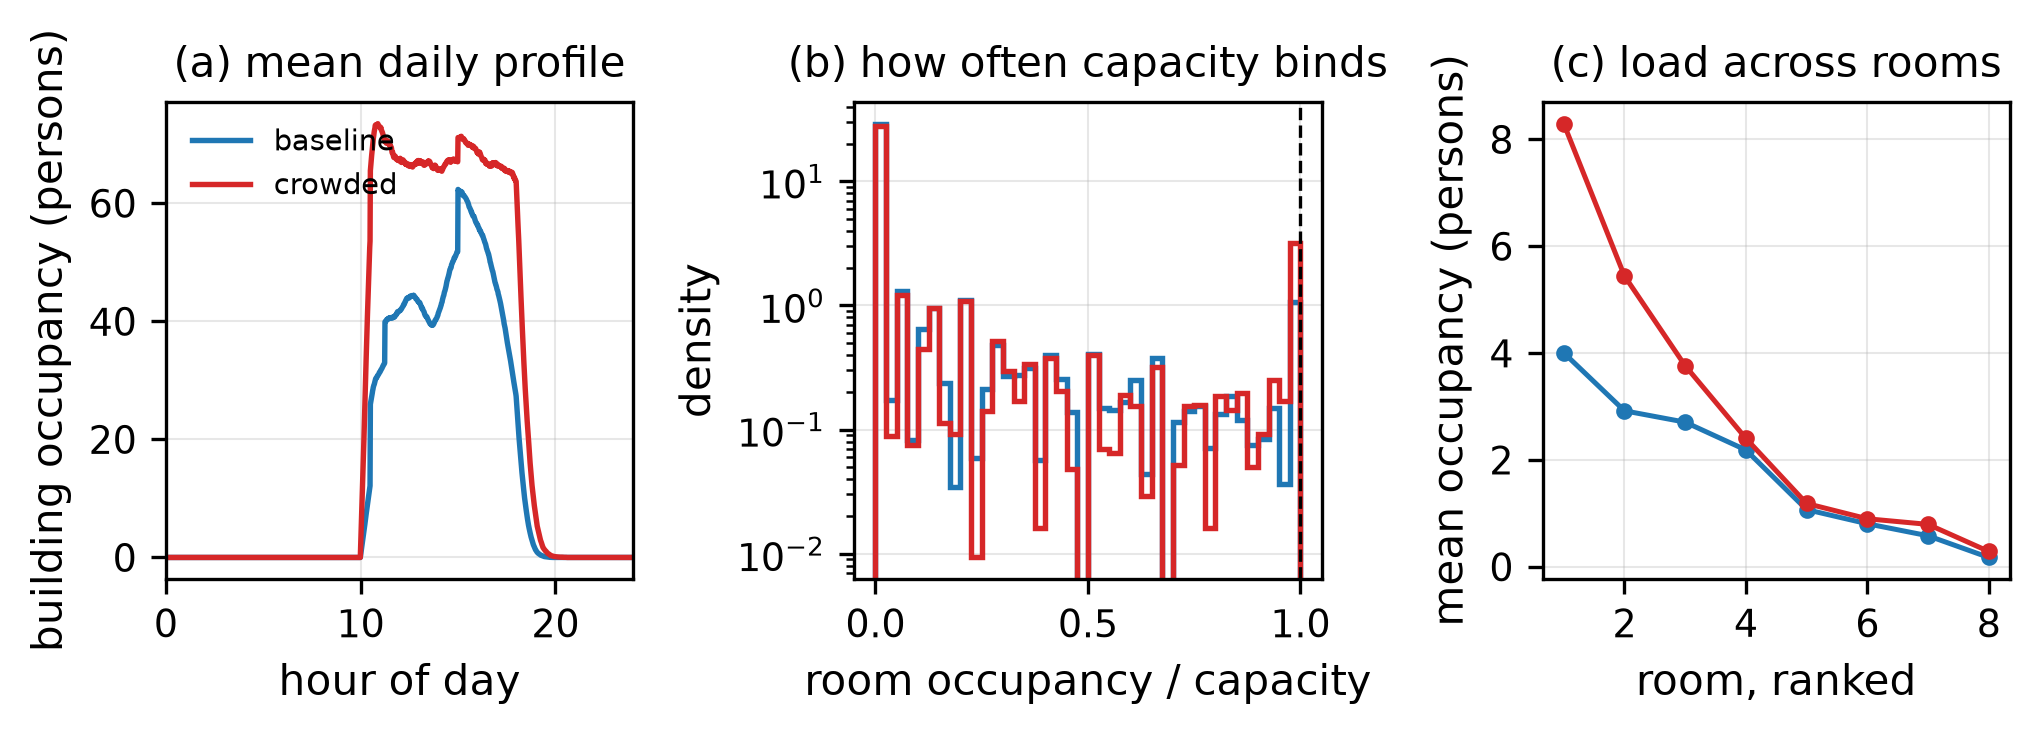
\includegraphics[width=0.96\textwidth]{figures/simulator_profile.png}
\caption{\new{What the simulator generates, at both operating points. (a) Mean occupancy of the whole building by time of day. (b) Distribution of room occupancy as a fraction of room capacity, log density; the dashed line is capacity and the crowded configuration puts visible mass on it. (c) Mean occupancy by room, ranked, showing that load is strongly unequal across the floor plan.}}
\label{fig:simprofile}
\end{figure}}

\subsection{Data efficiency and cost}
\label{sec:efficiency}

Figure~\ref{fig:efficiency} places the zero-shot model against a locally trained LightGBM given one to ninety days of site-specific data on the simulated museum. The trained model is already competitive at one day and saturates almost immediately, ending \SI{5.8}{\percent} ahead at \SI{60}{\minute}, moving only between \num{0.5926} and \num{0.5995} MASE across a ninety-fold change in the training budget. We had \new{stated a priori} a crossover of at least two weeks and it did not occur: on a simulated signal this clean, a local model learns essentially all there is to learn within a day. That is a failed prediction on our part and we report it as one.

\new{\paragraph{Is the real-data result explained by data scarcity? No.} The submitted version explained the trained model's weakness on ROBOD by the shortness of the record, calling it ``precisely the cold start the paper is about''. A reviewer objected that this had not been isolated: the weakness could equally be feature selection, tuning, the global training strategy or the handling of missing observations, and the submitted design varied none of them while varying the dataset. The objection is well founded and we tested the claim directly, holding the specification fixed and varying only the number of days of ROBOD history available for fitting. Panel (b) of Figure~\ref{fig:efficiency} reports it.}

\new{The explanation fails. Across a twenty-fold increase in the training budget, from three days to sixty, the trained model's MASE at one hour moves from \num{0.5544} to \num{0.5304} and back to \num{0.5392}, an improvement of at most \SI{4.3}{\percent} and not monotone. For comparison, the re-specification of Section~\ref{sec:lgbm} bought \SI{14.8}{\percent} on the same dataset at the same horizon. Specification mattered roughly three and a half times more than quantity, and twenty times the data closes less than a third of what changing the model's shape closes. Toto-2.0 at \num{0.3743} and last value at \num{0.5381} are invariant across the budgets by construction, since neither is fitted, and we verified that invariance as a check on the experiment rather than assuming it.}

\new{We therefore withdraw the data-scarcity explanation. What the ROBOD gap reflects is not that there is too little history to learn from but that a gradient-boosted model on lag and calendar features, however much of that history it is given, is a worse description of room occupancy than a pre-trained sequence model is. This is a more interesting claim than the one we made and a less comfortable one, because it does not support the cold-start framing that motivated the paper. The cold-start argument survives only in its narrow and still useful form: a newly instrumented building has no history at all, and a zero-shot model needs none, which is a statement about availability on day one rather than about the asymptotic value of data.}

It is worth being clear that \new{the simulator panel} points the opposite way to both real datasets, where the same family of trained model, given each site's full training split, was beaten at every horizon. The discrepancy is informative about the simulator rather than about the method. Our generator produces a stationary visitor process with no holidays, no exhibitions, no weather and no equipment faults, so ninety days of it contains far less novelty than ninety days of a real building, and a local model correspondingly has far less to be surprised by. The honest reading is that the data-efficiency figure gives an upper bound on how quickly a local model catches up, and the real datasets give the operationally relevant answer.

\begin{figure}[htbp]
\centering
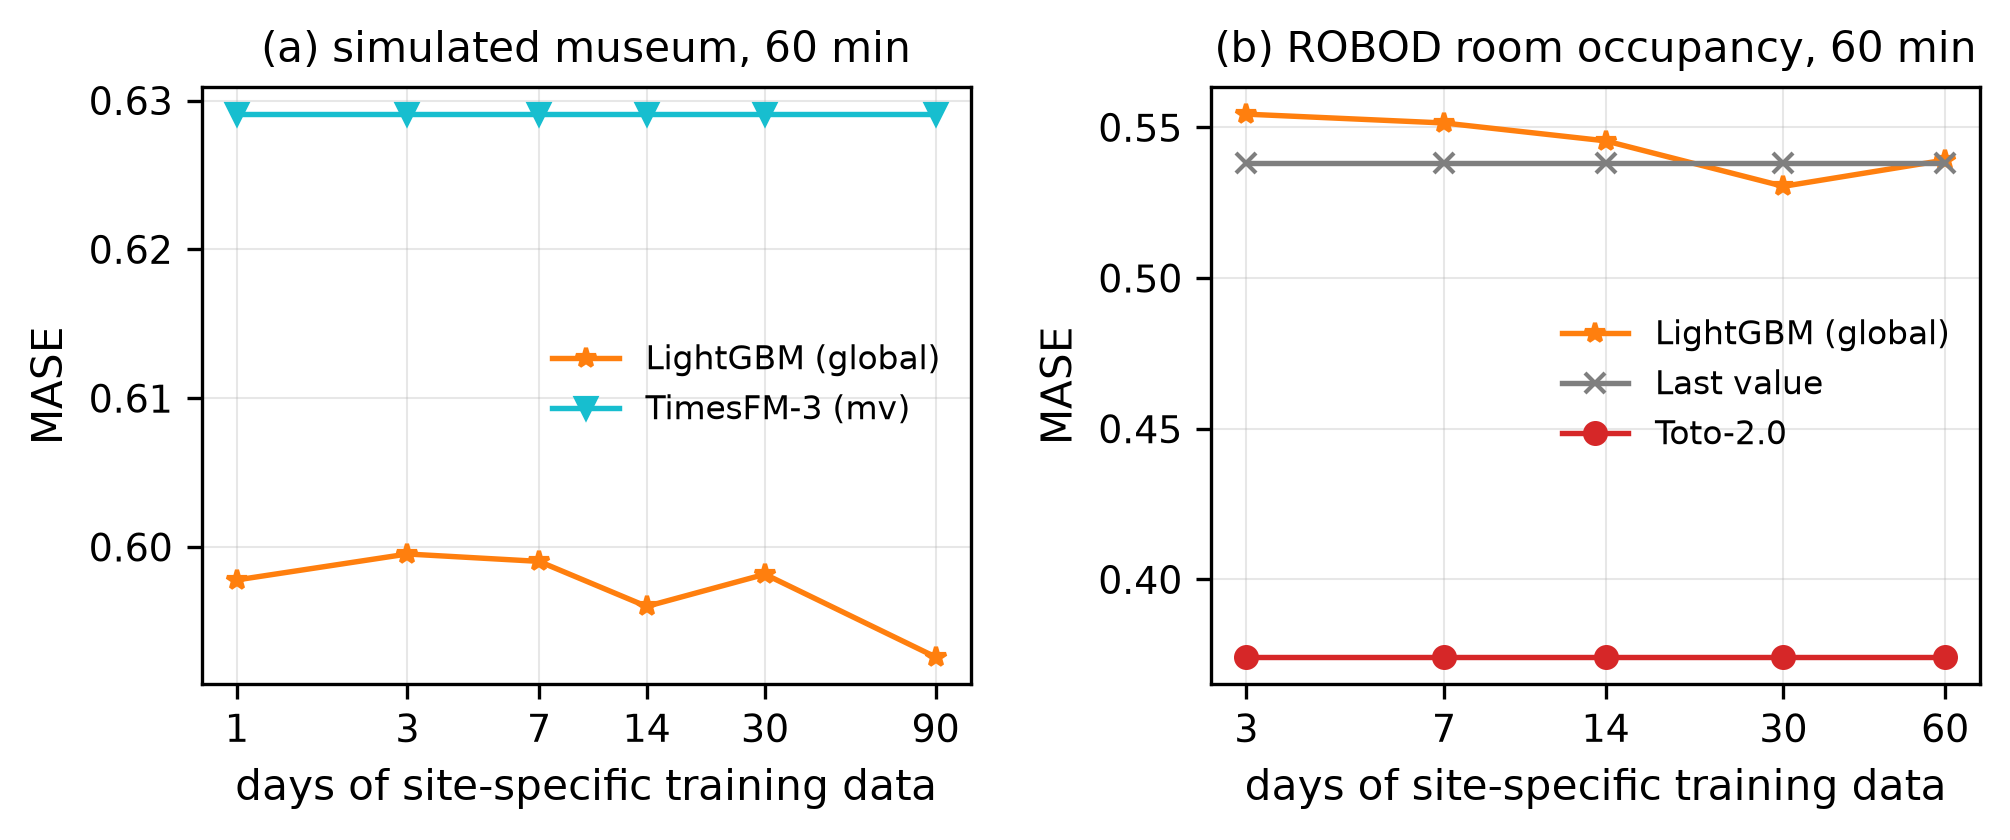
\includegraphics[width=0.96\textwidth]{figures/data_efficiency.png}
\caption{\new{Accuracy against the amount of site-specific training data, with the model specification held fixed so that only the budget varies. (a) The simulator, where a locally trained model saturates within a day, so the two-week crossover we stated a priori does not occur. (b) ROBOD, new in this revision, where twenty times more data buys at most \SI{4.3}{\percent} and leaves the trained model far short of the zero-shot one. Panel (b) is what refutes the data-scarcity explanation of the submitted version: if scarcity were the cause, this curve would descend towards the Toto-2.0 line, and it does not.}}
\label{fig:efficiency}
\end{figure}

\begin{figure}[htbp]
\centering
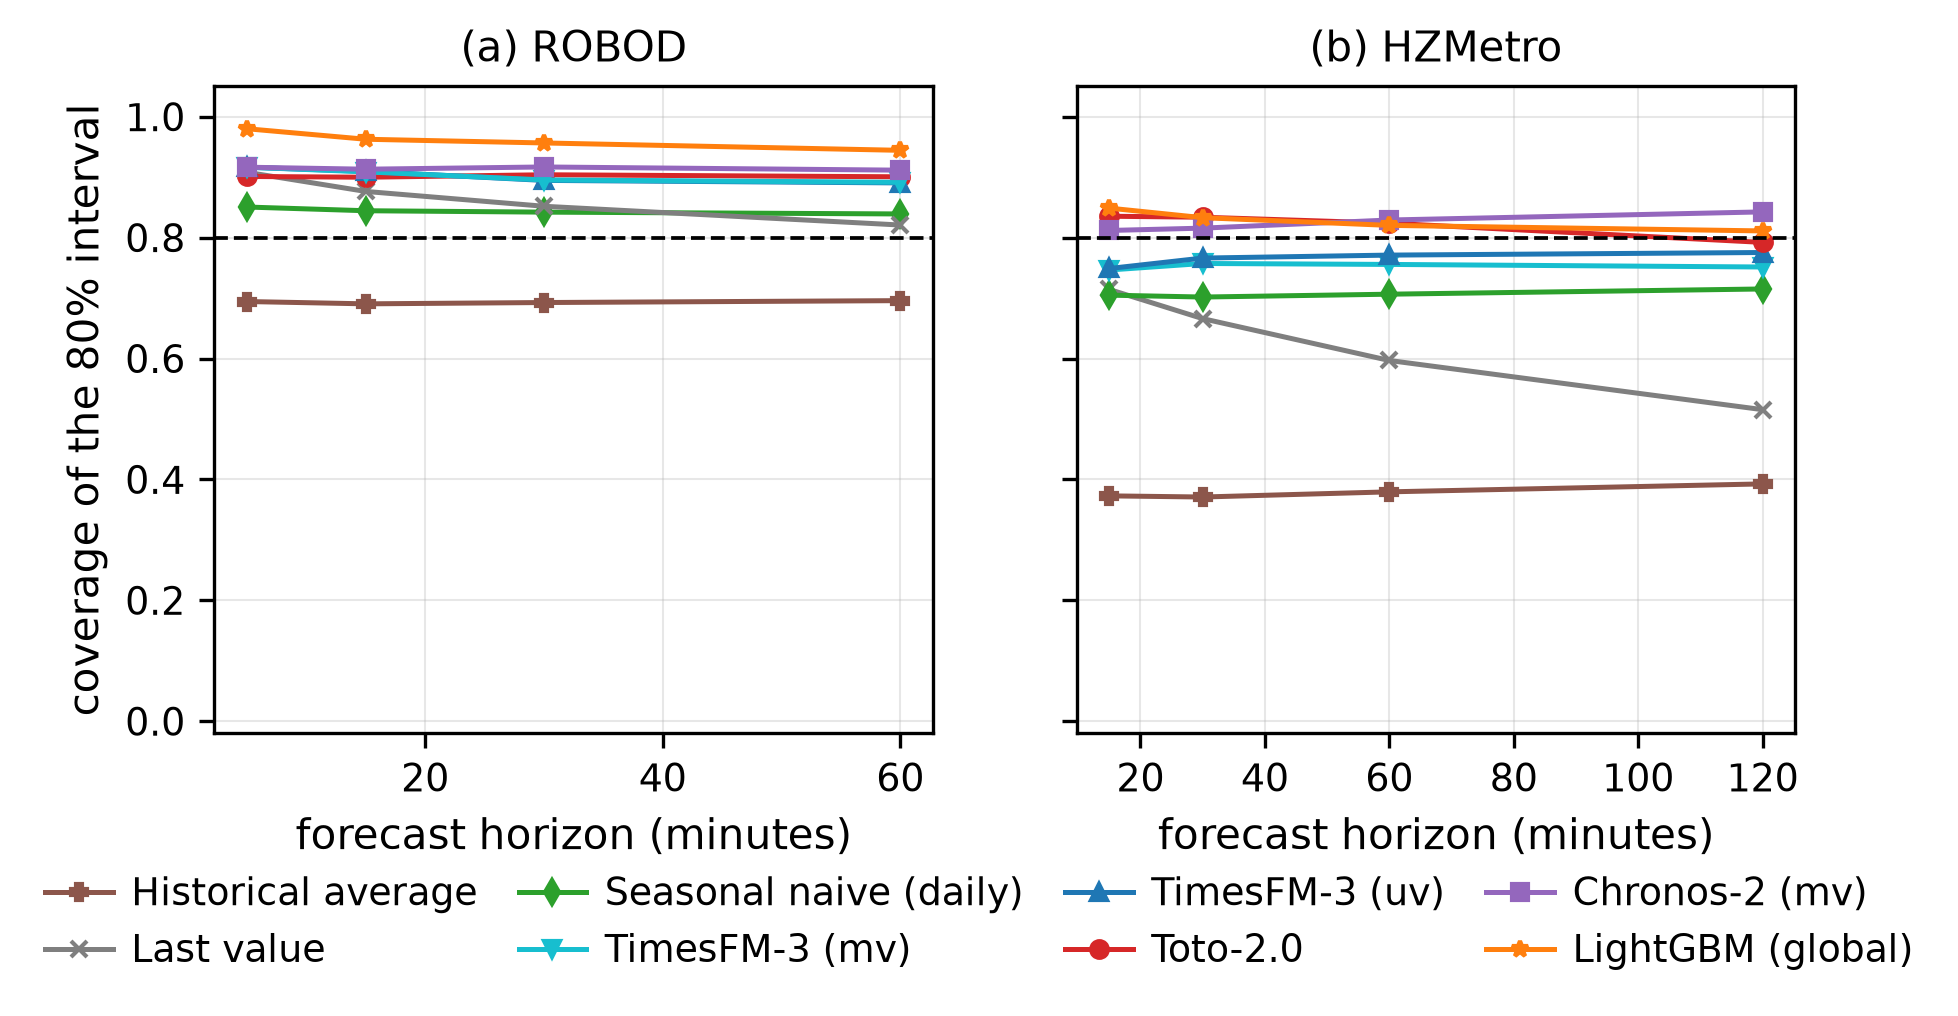
\includegraphics[width=0.92\textwidth]{figures/calibration.png}
\caption{Empirical coverage of the nominal \SI{80}{\percent} interval, dashed, against horizon on both real sites, with every method forming intervals from its own uncertainty. Coverage must be read together with the widths in Table~\ref{tab:calibration} and, for a comparison that means anything, with the matched-coverage widths in Table~\ref{tab:matched}.}
\label{fig:calibration}
\end{figure}

Cost is compatible with on-premise deployment, which matters because the privacy argument of Section~\ref{sec:related} depends on inference staying inside the building. On the \num{240}-series HZMetro panel at two seasons of context, the median per-origin latency on commodity hardware is \SI{269}{\milli\second} for Toto-2.0, \SI{302}{\milli\second} for Chronos-2 and \SI{303}{\milli\second} for TimesFM-3 multivariate, against \SI{16}{\milli\second} for seasonal naive and \SI{356}{\milli\second} for the trained LightGBM. The multivariate TimesFM-3 path is \num{2.5} times faster than its univariate path (\SI{748}{\milli\second}), since one forward pass replaces per-series calls. Reconciliation adds \new{\SI{6.2}{\milli\second} on the baseline configuration and \SI{7.2}{\milli\second} on the crowded one, measured as the \rev{median} wall-clock time of the OSQP solve}. A forecast plus projection therefore completes in well under a second at the scale of any museum, against horizons of tens of minutes.

Memory is the constraint that decides whether this runs on a building controller or needs a server, so it is worth stating what we can and cannot measure. Our harness records peak memory with \texttt{tracemalloc}, which counts Python heap allocations only. On the Apple Silicon hardware used here every tensor is held by the Metal allocator instead, so that column reports one to three megabytes for a transformer forward pass and is not a measurement of the model's footprint; we report it nowhere in this paper and have corrected the instrumentation. The figure a deployment needs is the peak resident set size of a process that loads one model and runs a single pass at the largest shape in this study, measured in isolation because a process high-water mark credits only whichever model allocates first. Measured that way, Chronos-2 peaks at \SI{1.04}{\gibi\byte}, TimesFM-3 at \SI{2.75}{\gibi\byte} in both modes and Toto-2.0 at \SI{2.92}{\gibi\byte}, against \SI{0.20}{\gibi\byte} for the trained LightGBM and \SI{0.10}{\gibi\byte} for the trivial baselines. That is comfortably within a modern edge device and decisively above a microcontroller, which is the practically relevant distinction.

\section{Discussion}
\label{sec:discussion}
\label{sec:disc}

\paragraph{What to deploy.}
\new{The submitted version of this paragraph recommended a frozen foundation model without qualification, on the grounds that it beat every local baseline we could afford to run. Section~\ref{sec:lgbm} removes that ground, and the recommendation this revision makes is conditional on something a practitioner can actually check before deploying.}

\new{What the evidence supports is the following. If no site-specific history exists, deploy a frozen foundation model, because it is the only option that produces a forecast at all and because its accuracy on both real sites is within the range a local model reaches only after being carefully specified. If a site has accumulated history and the engineering capacity to specify a local model properly, meaning seasonal lags, tuned hyper-parameters and a per-series fit, then the comparison is genuinely open and must be made on that site's own data: on metro station flow the local model won by \rev{\SI{16.6}{\percent}}, on room occupancy it lost by \rev{\SI{26.9}{\percent}, both by definition~\eqref{eq:relimp} on MASE}, and we can offer no statistic that predicts which case a new building falls into. We tried: the seasonal-strength statistic we proposed for exactly this purpose \rev{was not shown to} predict the advantage within a dataset (Section~\ref{sec:results}). The honest recommendation is therefore to use the zero-shot model as the cold-start default and to re-run the comparison locally once history exists, rather than to treat either paradigm as settled.}

\new{On the reconciliation layer, a reviewer judged our recommendation stronger than the evidence, and we accept the correction. The projection's guarantees are proved and hold for any admissible truth, so the case for applying \emph{some} topology constraint rests on mathematics rather than on our experiments. The case for our particular uncertainty weighting rests on measurements taken on simulated data only. Those measurements are consistent and the ablations of Section~\ref{sec:results} decompose them cleanly, but the effect sizes are small, around \SI{1}{\percent} of \rev{MAE}, and have not been reproduced on any real building. We therefore recommend the constrained projection on the strength of feasibility, which it guarantees at a cost of \SIrange{6}{7}{\milli\second}, and we offer the uncertainty weighting as the better-performing variant in our simulations rather than as an established improvement. A practitioner who adopted uniform weighting instead would lose, on our evidence, about one percent of accuracy and no guarantee. \rev{We also keep three kinds of claim apart, because Section~\ref{sec:risk} shows that they do not stand or fall together. Average accuracy improves slightly for one of the two forecasters. Among the risk-sensitive quantities, the error in the magnitude of the predicted peak falls by four to six percent, while the error at high occupancy and the detection of near-capacity and full-room conditions are essentially unchanged. An operational decision benefit, meaning better decisions by an operator acting on the reconciled forecast, was not evaluated and is not claimed. The recommendation to apply the projection therefore rests on feasibility and coherence, and not on improved identification of unsafe conditions.}}

\paragraph{How to evaluate.}
The finding with the broadest reach is not about any model. Section~\ref{sec:context} shows that the comparison between a foundation model and a seasonal baseline on periodic data reverses between one and two seasonal periods of context, while the baseline itself barely moves. A reader of a zero-shot leaderboard cannot recover this, and a context of one season is easy to choose by accident because it is the smallest at which a seasonal baseline is defined. The same choice starves that baseline's interval estimates, which turns a fair probabilistic comparison into a walkover. We would encourage reporting context length in units of the target's dominant season, and treating any zero-shot comparison against a periodic baseline as incomplete without a sensitivity check on it.

\paragraph{Why multivariate mode is not uniformly better.}
TimesFM-3 in multivariate mode beats its univariate path on ROBOD at every horizon, and loses to it on HZMetro at every horizon. We do not have a controlled ablation isolating the mechanism, since the covariate experiments of our original design did not run, and we therefore make no claim about cross-series attention beyond reporting the measurements. We flag it as the most immediate open question, and note the caution of \citet{shao2022stid} that apparent gains from cross-series structure often have a simpler explanation.

\paragraph{Limitations.}
\label{sec:limits}
No real heritage museum pilot is included, no real museum data appears anywhere in this paper, and we make no deployment claim for a gallery. \new{The title of the submitted version named heritage museums, which reviewers reasonably read as a claim about the evaluation data. We have changed it. The title now names the two physical quantities the method couples, occupancy and doorway flow, and the museum setting appears only where it belongs, as the motivating application and as the subject of the simulator we release.} The two real datasets are an instrumented office building and a metro network, chosen because they are the closest public analogues that exist: the first for indoor, bounded, directly counted room occupancy, the second for directional flow on a physical graph obeying the same continuity equation. Whether visitor behaviour in a gallery differs in ways that matter for forecasting is untested here and is the obvious thing to test next.

The reconciliation result rests on the simulator, and Remark~\ref{rem:admissible} gives the reason this is not merely a convenience: on real data the measured occupancies and doorway counts do not balance, because counters miscount, so the true future does not lie in the admissible set and the error-reduction guarantee weakens to the extent of that discrepancy. \new{We want to be unambiguous about the consequence, because it is the most important limitation in the paper. The proofs of Section~\ref{sec:method} hold unconditionally and are not contingent on any dataset. The empirical claim that the projection improves accuracy, and the ablations attributing that improvement to the uncertainty weighting rather than to the box constraints, hold on simulated data and nowhere else. Neither of the two real datasets can test them: ROBOD reports room occupancy without doorway counts, and HZMetro reports station flow without station occupancy, so in each case one side of~\eqref{eq:conservation} is missing and the constraint cannot be formed. We searched for a public dataset giving both for one building on a common clock and did not find one.}

\new{Obtaining such data is future work, and we can state what it requires rather than leaving it as an aspiration. The building needs synchronised counting at every doorway, including the ones leading outside, plus an independent occupancy estimate per room, since a doorway-derived occupancy would make the constraint hold by construction and test nothing. Fixed overhead depth or thermal sensors at each threshold with a separate per-room estimate would satisfy this, as would dense indoor positioning. Published pedestrian datasets of the ATC type come close in that they track individuals in a real indoor space, so a graph could be imposed on them after the fact, but they lack an occupancy measurement independent of the tracking and so inherit the same circularity. Until such a dataset exists, every reconciliation number in this paper should be read as a measurement of our simulator and not of a building.}

Separately, the simulator's data-efficiency result contradicts both real datasets on whether a trained local model catches up, which we read as a limitation of the generator's realism.

Two of our five hypotheses did not survive contact with the data in the form we stated them\new{, and a third survives only on one site}. The predictability hypothesis is \rev{not supported by the within-dataset analysis: the dependence it asserts is not statistically established, the confidence interval for the slope still contains negative values of practical size, and we neither rely on the hypothesis nor claim to have disproved it}. The interval comparison is supported \new{in \rev{a sharpness form on ROBOD, where the foundation model's interval is narrower than the seasonal one while covering more outcomes, is not established out of sample on HZMetro,} and \rev{is} refuted in its calibration form, since the seasonal baseline is closer to nominal coverage than any foundation model on ROBOD (Section~\ref{sec:calib}). The transferability hypothesis holds against a well-specified local model on ROBOD and fails on HZMetro (Section~\ref{sec:lgbm})}. We have kept \new{all of them} in the paper in their original form with the outcomes attached, rather than restating them to match what we found.

\new{Finally, the following experiments from our original design remain unrun, and no claim in this paper depends on them: the sensor-degradation study, so we say nothing about robustness to counter faults, drift or dropout; the covariate ablation, so we say nothing about whether known-future covariates help, despite the interface supporting them; and the decision-utility study, so we say nothing about operational lead time or about the three decision rules described in the introduction. A reviewer noted that our repository documentation described some of these as not executed while the manuscript appeared to report results from the same families, and we have corrected the documentation so that the experiment registry and this paragraph agree: the families reported here are the forecasting comparisons, the context and training-budget sweeps, and the reconciliation study, and the three listed above are absent from both. \rev{That correction had been made in our working copy and had not reached the public branch when the first revision was reviewed, as a reviewer found. It has now been published, and the Reproducibility statement identifies the tagged version of the repository that corresponds to this manuscript.}}

\paragraph{Ethics.}
The system counts and does not identify. Every claim rests on aggregate counts per space and per doorway, with no trajectories, no biometric data and no personal data leaving the building. This is a design constraint with a methodological consequence, since aggregate counting discards exactly the individual-level information trajectory methods rely on, which is why the problem is posed as forecasting on a graph. A deployment using device-based sensing would still warrant a data protection impact assessment under Article 35 of the GDPR \citep{gdpr}, and the same machinery would be open to misuse if paired with identifying sensors.

\section{Conclusion}

We asked whether a pre-trained time series foundation model can forecast occupancy and flow in a building it has never seen, and whether such a model can be made to respect the building's topology. \new{The two questions receive answers of very different strengths, and the main change in this revision is to stop stating them as though they were equally secure.}

\new{On the first question the answer is a qualified yes, and the qualification is not the one we anticipated. Given no site-specific training, the foundation models beat every trivial baseline on both real datasets, by \SI{30.5}{\percent} MASE at one hour on room occupancy and \SI{29.8}{\percent} at fifteen minutes on metro flow. Against a local gradient-boosted competitor the result splits by site: ahead by \rev{\SI{26.9}{\percent}} on room occupancy, behind by \rev{\SI{16.6}{\percent}} on metro flow\rev{, each the reduction in MASE of the better method relative to the worse,} once that competitor is given seasonal lags, tuned hyper-parameters and a per-series fit. The split is not an inconvenience to be averaged away, it is the finding, and it means the useful claim is that zero-shot forecasting is a competitive default under a cold start rather than a uniformly superior method. Two further qualifications matter as much. The comparison against a seasonal baseline is decided by context length: at one seasonal period of history the foundation models lose on metro flow, at two they win by a third, while the baseline itself does not move, and accuracy keeps improving to about seven seasons. And under a moving-block bootstrap that respects the overlap between forecast origins, the confidence interval for the foundation model's advantage over the seasonal baseline at the longest metro horizon contains zero, so that particular advantage is not statistically established even where the pointwise test rejects. Any zero-shot evaluation on periodic data that does not report and vary its context length, and does not account for dependence between overlapping origins, is reporting a property of its configuration.}

\new{Two of our own hypotheses \rev{were not borne out}, and both \rev{outcomes} are more useful than the claims would have been.} The prediction that the advantage declines with the target's seasonal strength \rev{is not supported by} a within-dataset test on \num{160} \new{scored} series\rev{: the slope is negative, as predicted, but its confidence interval, $[-38,+4]$ percentage points per unit of seasonal strength, includes both zero and declines of practical size, so the dependence is not statistically established and we make no claim that rests on it}; the between-dataset ordering that appeared to support it was close to a restatement of the definition of the statistic. \new{The prediction that foundation models are better calibrated is also withdrawn: the seasonal baseline is nearer nominal coverage, and what survives is a sharpness claim \rev{on room occupancy, where the foundation model's interval is half as wide as the seasonal one while covering more outcomes, and where the seasonal interval must be widened \num{6.0} times retrospectively, or \num{8.4} times with a scale factor estimated on a preceding calibration period, to reach a common coverage near \SI{90}{\percent}. The corresponding advantage on metro flow holds retrospectively and is not established out of sample}.}

On the second question the answer \new{is affirmative as mathematics and provisional as measurement, and the distinction is the point}. The uncertainty-weighted constrained projection is unique, exactly coherent, and provably non-expansive towards any admissible truth, with MinT recovered exactly as the special case that discards the inequality constraints and, as predicted and then measured, breaks them by \num{2.06} persons per origin, rising to \num{2.94} in a scenario where capacity actually binds. Raw forecasts violate conservation by \num{1.05} persons per node per interval; the projection removes this in \SI{6.2}{\milli\second} while improving point accuracy, and the ablations isolate where that improvement comes from: the uncertainty weighting contributes about \SI{1}{\percent} of \rev{MAE} and the inequality constraints about \SI{0.3}{\percent}. \rev{Against the raw forecast the reduction in mean error is statistically established for TimesFM-3 and not for LightGBM, and for TimesFM-3 it coexists with a very slight and equally well established deterioration at the typical origin, so it is a statement about the mean and not about most forecasts.} \new{Three boundaries on this half of the paper should travel with it. Every one of these empirical numbers comes from the simulator, because no public dataset reports occupancy and doorway flow for the same building, so the reconciliation layer is demonstrated rather than validated and real-building validation is the principal item of future work. The guarantee covers the projected median path and not the whole predictive distribution: under the default shift strategy the non-median quantiles are translated by the median correction and remain mildly incoherent, by \num{0.085} persons in residual at the \rev{\num{90}th} percentile\rev{. Projecting each quantile separately does not close this gap: the independently projected levels are each coherent and feasible but cross on \SI{11.3}{\percent} of adjacent pairs, and the rearrangement that restores their order leaves residuals of \num{0.003} to \num{0.012} persons, at the median included, so quantile paths that are individually admissible are not a coherent joint distribution. And the risk-sensitive evidence is narrower than an earlier version of this conclusion stated. The error in the magnitude of the predicted peak falls by \SI{6.3}{\percent}, against \SI{0.56}{\percent} for mean absolute error, and that reduction is statistically established; but the detection of near-capacity and full-room conditions is essentially unchanged, with hit rates moving by between \num{0.2} and \num{1.3} percentage points, and the error at high occupancy is not consistently improved. A more accurate peak magnitude is not improved identification of unsafe conditions, and neither is a demonstrated operational benefit, which would require the decision study that remains unrun}.} We release the simulated benchmark, the reconciliation layer and the harness, in which every reported number is traceable to a logged run.


\section*{Reproducibility statement}

All experiments are driven by versioned configuration files. Each run writes a manifest with the git commit, configuration hash, seed, package versions and hardware, alongside per-origin predictions and metrics. Every figure and table here is generated by one script from those artefacts, and it fails rather than emitting a placeholder when a run is missing. Public datasets are fetched by per-source scripts that record download date and checksum; the data itself is not redistributed.

\new{A reviewer asked us to correct a word. The submitted version described our hypotheses as ``pre-registered''. They were not: they were written down in the repository before the corresponding experiments were run, and the commit history evidences that, but they were never deposited with any registry, and ``pre-registered'' is a term of art that implies a third-party time-stamped record. We have replaced it with ``stated a priori'' throughout, which is what we are in a position to claim.}

\new{The same reviewer noted that we declared data availability as not applicable while also supplying a code repository, which is inconsistent. The statement below resolves it.} All the codes are publicly accessible via: \url{https://github.com/001shahab/zero-shot-FMF}

\rev{A reviewer of this revision found that the public repository had not been brought into line with the revised manuscript: its documentation still described most experiments as not executed, retained results from the first submission and referred to three seeds. The observation was correct. The corrections described in our previous response had been made in the working copy and had not been published to the public branch. The repository has now been updated, and the version corresponding to this manuscript is identified by the tag \texttt{manuscript-r2}. At that tag the README states which experiment families were run and which were not, in agreement with Section~\ref{sec:limits}; it reports the results of this manuscript and no others; it states that the forecasters are deterministic, so that repeated seeds reproduce identical forecasts and the reported counts are counts of distinct origins and not of seed replicates; and it lists the configuration file behind every table. The analyses added in this revision are generated by the script \texttt{analysis\_round2.py} from the logged predictions, written to \texttt{summary\_round2.json}, and checked against the text of the manuscript by \texttt{verify\_round2.py}, which fails if any number quoted here differs from the logged value.}

\section*{Conflict of Interest Statement}

The authors declare that the research was conducted in the absence of any commercial or financial relationships that could be construed as a potential conflict of interest.

\section*{Author Contributions}

A. A. Jafari was contributing to: Conceptualization, Formal analysis, Investigation, Methodology, Software, Visualization, Writing -- original draft, and Writing -- review \& editing. C. Ozcinar was contributing to: Conceptualization, Formal analysis, Methodology, Supervision, Validation, and Writing -- review \& editing. G. Anbarjafari was contributing to: Conceptualization, Formal analysis, Investigation, Methodology, Supervision, Validation, Writing -- original draft, and Writing -- review \& editing.

\section*{Acknowledgment}
\new{The authors thank the authors of the ROBOD and PVCGN releases for making their datasets publicly available, and the developers of TimesFM, Chronos and Toto for releasing model weights and inference code without which a zero-shot study of this kind could not be run. We also thank the anonymous reviewers, whose objections changed several of this paper's conclusions rather than only its presentation: the strengthened local competitor, the separation of calibration from sharpness, the dependence-aware confidence intervals and the explicit statement of what is and is not tested on real data all follow from their comments.}

\bibliographystyle{Frontiers-Harvard} 
\bibliography{ref}



\end{document}
